\documentclass[12pt,a4paper,oneside]{scrbook}
\usepackage{graphicx} % do dodawania zdjęć
\usepackage[utf8]{inputenc}
\usepackage[T1]{fontenc}
\usepackage[margin=2.5cm]{geometry}
\usepackage{setspace}
\setstretch{1.5}
\usepackage{lmodern}
\usepackage[polish]{babel}
\usepackage[autostyle=true]{csquotes}
\usepackage{amsmath}
\usepackage{amssymb}
\usepackage{caption}
\usepackage{subcaption}
\usepackage{url}
\usepackage{siunitx}
\usepackage{microtype}
\usepackage{svg}
\usepackage{pdfpages}
\usepackage{wrapfig}
\usepackage{booktabs}
\usepackage[most]{tcolorbox} % dla kart z interpretacją cech w aneksie
\usepackage{tikz}
\usetikzlibrary{positioning}
\sisetup{output-decimal-marker = {,}}
\sisetup{group-separator = {\,}}

\setlength{\skip\footins}{1.2cm}

\begin{document}
% Logo AGH
\thispagestyle{empty}
\begin{figure}[ht]
    \centering
    
\includegraphics[width=0.9\textwidth]{images/agh_logo.jpg}
\end{figure}
\vspace{-0.41cm}
\begin{center}
    \textbf{\fontsize{9.5}{9}\selectfont
    \begin{tabular}{@{}c@{}} % @{} usuwa dodatkowe marginesy w tabular
    WYDZIAŁ ELEKTROTECHNIKI, AUTOMATYKI, INFORMATYKI I INŻYNIERII\\
    BIOMEDYCZNEJ
    \end{tabular}}
\end{center}
    

% Tytuł pracy
\vspace{1.7cm}
\begin{center}
    \textbf{\Huge Praca dyplomowa} \\
    \vspace{1.5cm}
    \textbf{\large Identyfikacja i wizualizacja reprezentacji faktów w strukturze modeli językowych -- analiza zależności i zastosowania w budowie wyspecjalizowanych modeli} \\
    \vspace{1cm}
    \textbf{\large Identification and Visualization of Fact Representations in Language Model Structures -- Dependency Analysis and Applications in Domain-Specific Model Development}
\end{center}

\vspace{1.5cm}
\begin{addmargin}[1cm]{1cm}
    \begin{tabbing}
        \textbf{Autor:} \hspace{3.5cm} \=  inż. Eryk Mikołajek \\
        \textbf{Kierunek studiów:} \> Informatyka i Systemy Inteligentne \\
        \textbf{Opiekun pracy:} \> dr hab. Adrian Horzyk \end{tabbing}
\end{addmargin}

\vspace{1.5cm}
\begin{center}
    Kraków, 2026
\end{center}

\tableofcontents

\chapter{Wstęp}
Ostatnie lata przyniosły gwałtowny rozwój dużych modeli językowych, których zdolności w zakresie rozumienia i generowania języka naturalnego przekroczyły to, czego jeszcze dekadę wcześniej można się było spodziewać po systemach sztucznej inteligencji. Powszechna dostępność takich modeli w formie aplikacji konwersacyjnych sprawiła, że temat ten -- dotąd obecny głównie w środowisku naukowym -- stał się przedmiotem szerokiego zainteresowania opinii publicznej, przemysłu oraz badaczy z wielu dziedzin. Wzrost ten nie był przełomem naukowym sam w sobie, lecz katalizatorem: nasilił globalną ciekawość, w jaki sposób modele te faktycznie przetwarzają informacje i co dokładnie kryje się w ich wewnętrznej strukturze. Niniejsza praca dyplomowa stanowi próbę częściowego zaspokojenia tej ciekawości, przedstawiając proces badania tego zjawiska oraz możliwości wykorzystania zdobytej w ten sposób wiedzy do optymalizacji samych modeli.

\section{Motywacja}
\label{sec:motywacja}
Sztuczne sieci neuronowe (ang. \textit{Artificial Neural Networks}) stanowią dziś architekturę bazową dla większości modeli sztucznej inteligencji. Zbudowane z ogromnej liczby prostych jednostek obliczeniowych -- neuronów -- sieci te zawdzięczają swoją skuteczność zdolności do plastycznego dostosowywania się do stawianych przed nimi zadań w procesie treningu. Ta sama elastyczność jest jednak źródłem podstawowego ograniczenia: sieci neuronowe pozostają w praktyce czarnymi skrzynkami (ang. \textit{black box}) -- na wejściu dostarczane są dane, na wyjściu otrzymywany jest wynik, natomiast sposób, w jaki ten wynik powstaje, nie jest bezpośrednio i w pełni obiektywnie interpretowalny. Badacze mogą jedynie pośrednio wnioskować o skutkach aktywacji poszczególnych neuronów, stawiając hipotezy co do przyczyn ich pobudzenia. \newline
Zainteresowanie tym zjawiskiem nie jest nowe -- pytanie o to, w jaki sposób sieci neuronowe przetwarzają i reprezentują informacje, towarzyszy tej dziedzinie od dawna. Istotnie nasiliło się ono jednak wraz z pojawieniem się dużych modeli językowych, trenowanych na ogromnych zbiorach danych tekstowych i w rezultacie dysponujących dostępem do rozległej wiedzy -- w tym takiej, która nie powinna być powszechnie dostępna lub swobodnie wykorzystywana. Z tego powodu szczególnego znaczenia nabrało zrozumienie, w jaki sposób modele te \enquote{myślą} oraz w jaki sposób można świadomie kształtować ich zachowanie -- wzmacniając pożądane wzorce i osłabiając te niepożądane. Poddziedzina zajmująca się tego rodzaju analizą wewnętrznej struktury sieci neuronowych nazywana jest mechanistyczną interpretowalnością (ang. \textit{mechanistic interpretability}); choć wywodzi się ona z badań nad sieciami znacznie prostszymi niż współczesne modele językowe, to właśnie w kontekście tych ostatnich zyskała w ostatnich latach szczególne znaczenie praktyczne. \newline
Wiedza ta niesie ze sobą również potencjał praktyczny, wykraczający poza czysto poznawczy cel zrozumienia modelu, a powodów, dla których jest ona istotna, jest wiele. Z perspektywy bezpieczeństwa, wgląd w to, jakie wzorce zachowań model faktycznie wykorzystuje, pozwala wykryć te niepożądane, zanim ujawnią się one w praktycznym zastosowaniu. Z perspektywy praktycznej -- umożliwia lokalizowanie źródeł błędów czy niepożądanych korelacji wyuczonych przez sieć, a więc świadome debugowanie modelu, czego nie sposób osiągnąć, traktując go jako czarną skrzynkę. \newline
Trzecia motywacja, najbliższa tematyce niniejszej pracy, dotyczy optymalizacji: jeżeli da się wskazać, które komponenty sieci realizują istotne obliczenia, a które są względem zadania redundantne, otwiera to drogę do świadomego upraszczania modeli bez utraty ich funkcjonalności -- zarówno poprzez zmniejszenie ich zapotrzebowania na moc obliczeniową, jak i stworzenie mniejszych, wyspecjalizowanych wariantów dostosowanych do konkretnych zastosowań.

\section{Cele}
\label{sec:cele}
Pierwszym celem pracy jest lokalizacja i wizualizacja reprezentacji wiedzy faktycznej wyuczonej przez model językowy. Obiektem badań będzie mały, otwarto-źródłowy model językowy oparty na architekturze dekodera. Podobnie do podejść stosowanych w pracach \cite{templeton_scaling_monosemanticity} i \cite{lanza_extraction_analysis_multimodal_concepts}, do ekstrakcji cech reprezentacji wewnętrznych zastosowany zostanie Rzadki Autoenkoder (ang. \textit{Sparse Autoencoder} -- SAE), a konkretnie jego wariant Top-K \cite{gao_2024_scaling_evaluating_sparse_autoencoders}. Metoda ta pozwala uzyskać rzadkie, bardziej monosemantyczne rozkłady aktywacji, dając wgląd w to, jakie koncepty model \enquote{rozumie}, jak są one ze sobą powiązane i w jaki sposób grupuje on informacje w swojej wewnętrznej reprezentacji. Zebrane w ten sposób dane stanowią fundament dla kolejnych etapów pracy. \newline
Dysponując mapą konceptów wyuczonych przez model, zbadana zostanie możliwość wydzielenia z niego węższych modeli dziedzinowych za pomocą techniki przycinania (ang. \textit{pruning}). Modele takie, ograniczone do wybranej domeny wiedzy, miałyby zachowywać zbliżoną jakość w obrębie tej dziedziny przy jednoczesnej redukcji liczby parametrów i kosztów obliczeniowych. Efekt ten zostanie osiągnięty przez semantyczną klasyfikację wyekstrahowanych cech, a następnie usunięcie komponentów modelu nieistotnych dla wybranej domeny. \newline
Uzupełniająco zbadana zostanie możliwość innego wykorzystania wyznaczonych domen -- jako ekspertów w architekturze mieszaniny ekspertów (ang. \textit{Mixture of Experts}, MoE) \cite{jacobs_1991_adaptive_mixtures_of_local_experts}. W odróżnieniu od konwencjonalnych podejść do budowy modeli MoE, w których eksperci wyłaniani są w procesie treningu, w niniejszej pracy zbadana zostanie możliwość zdefiniowania ekspertów poprzez wydzielone, interpretowalne domeny wiedzy, wyznaczone na podstawie analizy cech SAE.

\section{Hipotezy i pytania badawcze}
\label{sec:hipotezy_pytania}
Realizacja celów przedstawionych w poprzedniej sekcji opiera się na czterech hipotezach badawczych. Każda z nich formułuje konkretne oczekiwanie co do własności reprezentacji wiedzy w modelu lub co do możliwości praktycznego ich wykorzystania; każdej towarzyszy odpowiadające pytanie badawcze wyznaczające zakres empirycznej weryfikacji.
\begin{enumerate}
    \item \textbf{Fakty i koncepty posiadają identyfikowalne reprezentacje w wewnętrznej strukturze modelu językowego.}
    Modele językowe nabywają wiedzę wyłącznie poprzez trening na tekście -- nie mają dostępu do żadnych zewnętrznych baz wiedzy ani słowników. Oznacza to, że informacje, które model jest w stanie poprawnie przywołać, muszą być zakodowane gdzieś w jego parametrach. Założenie o identyfikowalności tych reprezentacji jest zatem warunkiem wstępnym całego dalszego programu badawczego.
    \textit{Pytanie badawcze:} W jaki sposób można lokalizować i identyfikować reprezentacje wiedzy faktycznej w wewnętrznej strukturze modelu językowego?
    \newpage
    \item \textbf{Fakty powiązane semantycznie wykazują zbliżone lub sąsiadujące reprezentacje w przestrzeni wewnętrznej modelu.}
    Skoro model uczy się na podstawie wzajemnego współwystępowania słów i pojęć w tekście, fakty należące do tej samej dziedziny były mu wielokrotnie przedstawiane w podobnych kontekstach. Można zatem oczekiwać, że ich wewnętrzne reprezentacje będą geometrycznie zbliżone. Jest to zarazem warunek niezbędny do tego, by wiedza dziedzinowa dawała się sensownie wydzielić w kolejnych etapach pracy.
    \textit{Pytanie badawcze:} Czy fakty o podobnym znaczeniu wykazują wzajemne sąsiedztwo w przestrzeni wewnętrznej modelu i w jaki sposób można tę strukturę zmierzyć i zwizualizować?
    \item \textbf{Możliwe jest wydzielenie wąskiej dziedziny wiedzy z modelu poprzez technikę przycinania, z zachowaniem jakości w obrębie tej dziedziny.}
    Jeżeli wiedza faktyczna jest identyfikowalna i wykazuje przestrzenną spójność (hipotezy 1 i 2), to selektywne usuwanie komponentów modelu nieistotnych dla wybranej domeny powinno być możliwe bez poważnego pogorszenia jego wyników w zakresie tej domeny. Stopień, w jakim jest to faktycznie osiągalne, zależy od tego, na ile poszczególne dziedziny wiedzy są w modelu rozłączne..
    \textit{Pytanie badawcze:} Jakie są granice możliwości izolowania wiedzy dziedzinowej z modelu językowego poprzez technikę przycinania i jak mierzyć utratę jakości wynikającą z tego procesu?
    \item \textbf{Wyznaczone domeny wiedzy mogą stanowić podstawę do zdefiniowania ekspertów w architekturze MoE.}
    Jeżeli dziedziny wiedzy można wydzielić i opisać w sposób interpretowalny, stanowią naturalnych kandydatów na ekspertów w architekturze, w której przy każdym zapytaniu aktywuje się tylko ta część modelu kompetentna w danej dziedzinie. Takie podejście różni się od rozwiązań konwencjonalnych tym, że eksperci byliby zdefiniowani przez jawne kryteria semantyczne, a nie wyłaniani automatycznie w procesie treningu.
    \textit{Pytanie badawcze:} W jakim stopniu domeny wiedzy wyznaczone na podstawie analizy reprezentacji modelu mogą pełnić funkcję ekspertów w architekturze MoE?
\end{enumerate}

\chapter{Wprowadzenie teoretyczne}
W poniższym rozdziale omówiona zostanie krótko historia badań nad interpretowalnością sieci neuronowych. W szczególności analiza, w tym kontekście, sieci konwolucyjnych (ang. \textit{Convolutional Neural Networks}). Przybliżona zostanie także architektura sieci typu transformer oraz jej rola w modelach językowych. W dalszej części opisana zostanie literatura skupiająca swoją uwagę na badaniu interpretowalności modeli językowych oraz rola Rzadkich Autoenkoderów (ang. \textit{Sparse Autoencoders}) w ekstrakcji cech. Na koniec omówione zostaną modele typu MoE (ang. \textit{Mixture of Experts}), sposoby ich budowania oraz możliwość zastosowania w owej pracy.

\section{Interpretowalność sieci neuronowych}
\label{sec:interpretowalnosc_sieci_neuronowych}
Sieci neuronowe zbudowane są ze sztucznych neuronów -- prostej jednostki przetwarzającej wartości otrzymane na wejściu od połączonych z nią neuronów i produkującej na wyjściu wartość swojego pobudzenia. Każdy neuron przypisuje do każdego innego połączonego z nim neuronu wagę, posiada własny parametr przesunięcia (ang. \textit{bias}) oraz nieliniową funkcję aktywacji. Mnożąc każde wejście przez odpowiadającą mu wagę, następnie dodając wartość przesunięcia i na koniec stosując funkcję aktywacji, dostaje na wyjściu liczbę, która jest wartością jego aktywacji. W sieciach neuronowych, zwłaszcza w większych modelach, połączonych ze sobą w warstwy są miliony, lub nawet miliardy neuronów. Każdy neuron aktywuje się w odpowiedzi na inny sygnał lub zestaw sygnałów, a grupy neuronów przetwarzających sygnały w podobny do siebie sposób są rozproszone po całej sieci. Cały ten szereg komplikacji sprawia, że nie da się w prosty i jednoznaczny sposób odpowiedzieć na pytania dlaczego sieć dała konkretną odpowiedź, lub jaki proces doprowadził do danego wyniku. \newline
Powstało wiele podejść tworzenia i badania mechanizmów wyjaśniających sposoby działania złożonych modeli. Zgodnie z podziałem literatury w artykule przeglądowym autorstwa Tilmana Räukera \cite{rauker_toward_transparent_ai}, tradycyjne podejścia w ramach wyjaśnialnej sztucznej inteligencji (ang. \textit{Explainable AI}) opierają się głównie na metodach post-hoc, które traktują model jak czarną skrzynkę. Metody te próbują wyjaśnić decyzje modelu na podstawie analizy jego wejść i wyjść, odpowiadając m.in. na pytanie jakie próbki lub cechy w najbardziej znaczący sposób wpływają na wynik modelu. Pomaga to zrozumieć zależności przyczynowo-skutkowe pomiędzy danymi wejściowymi a wynikami modelu. W opozycji do tego stoi poddziedzina nazywana mechanistyczną interpretowalnością (ang. \textit{mechanistic interpretability}), które skupia się na wewnętrznej strukturze modelu. To podejście wykorzystuje proces inżynierii odwrotnej sieci neuronowej na poziomie pojedynczych neuronów i ich połączeń. Pozwala to zrozumieć wewnętrzną logikę i mechanikę działania modelu. Odpowiada na pytanie w jaki sposób jego poszczególne komponenty (takie jak węzły i wagi w modelach głębokich sieci neuronowych) generują odwzorowanie pomiędzy danymi wejściowymi a wynikiem działania systemu. \newline
Niniejsza praca w przeważającej większości korzysta z podejścia mechanistycznego. Wybór ten wynika z ograniczeń, jakie niesie ze sobą klasyczne podejście post-hoc. Cynthia Rudin w pracy \cite{rudin_stop_explaining_black_box_machine_learning_models} argumentuje, że wyjaśnienia nakładane na czarną skrzynkę po fakcie są jedynie przybliżeniem rzeczywistego działania modelu -- gdyby odwzorowywały je w pełni wiernie, same stałyby się tym modelem, co czyni je z definicji częściowo niedokładnymi. W kontekście decyzji o wysokiej stawce, w obliczu jakich stawia się obecnie modele sztucznej inteligencji, tj. diagnozy medyczne czy wyroki sądowe, wymagana jest większa wierność wyjaśnianych elementów. Mechanistyczna interpretowalność podąża inną drogą: próbuje wiernie zrekonstruować mechanizm, który już wewnątrz sieci istnieje. Ponieważ opiera się na bezpośredniej analizie wag i aktywacji, a nie na przybliżeniach formułowanych wyłącznie na podstawie wejść i wyjść, pozwala uniknąć problemu utraty wierności. \newline
Szersze motywacje stojące za potrzebą interpretowalności -- obejmujące zarówno bezpieczeństwo systemów sztucznej inteligencji, jak i możliwości optymalizacji architektur -- zostały omówione w rozdziale~\ref{sec:motywacja}; tu wystarczy zaznaczyć, że mechanistyczna interpretowalność odpowiada na nie w sposób, którego podejście post-hoc z definicji nie może zapewnić.


\section{Wczesne prace nad wizualizacją i interpretacją głębokich sieci neuronowych} 
\label{sec:wczesne_prace_wizualizacja}
W 2006 roku Geoffrey Hinton wraz ze współpracownikami opublikował dwa przełomowe artykuły, które zapoczątkowały tzw. renesans głębokiego uczenia (ang. \textit{deep learning}). Wykazano w nich, że wielowarstwowe sieci neuronowe -- dotąd trudne do skutecznego trenowania metodą propagacji wstecznej ze względu na problem zanikającego gradientu i słabą jakość znajdywanych minimów -- można efektywnie uczyć dzięki wstępnemu, nienadzorowanemu trenowaniu warstwa po warstwie z wykorzystaniem Maszyn Boltzmanna z ograniczeniami (ang. \textit{Restricted Boltzmann Machines, RBMs}) \cite{hinton_reducing_the_dimensionality_of_data} \cite{hinton_a_fast_learning_algorithm_for_deep_belief_nets}. Niemal równolegle analogiczną, zachłanną metodę wstępnego trenowania, opartą na autoenkoderach, rozwijał zespół Yoshuy Bengio \cite{lamblin_greedy_layer_wise_training_of_deep_networks}. \newline
Sukces w trenowaniu głębokich architektur postawił nowe pytanie badawcze: co właściwie poszczególne warstwy sieci uczą się reprezentować? Dotychczasowe prace poświęcone interpretacji sieci neuronowych ograniczały się zasadniczo do pierwszej warstwy, której wagi -- traktowane jako filtry w przestrzeni wejściowej -- dawało się przedstawić w postaci obrazów przypominających m.in. detektory krawędzi lub filtry Gabora. Interpretacja warstw głębszych pozostawała znacznie trudniejsza, ponieważ ich reprezentacji nie można było odczytać w równie bezpośredni sposób. \newline
Pierwsze próby wyjścia poza pierwszą warstwę podjęli Honglak Lee i współpracownicy, którzy -- opierając się na architekturze Deep Belief Networks zaproponowanej przez Hintona -- wizualizowali cechy drugiej warstwy sieci metodą liniowej kombinacji filtrów warstwy poprzedzającej \cite{lee_sparse_deep_belief_net_model_for_visual_area_v2}, a rok później rozszerzyli tę technikę na trzecią warstwę w kontekście konwolucyjnego wariantu tej architektury \cite{lee_convolutional_deep_belief_networks_for_scalable_unsupervised_learning}. \newline
Punktem przełomowym dla systematycznego badania cech wyższych warstw stała się jednak dopiero praca \textit{Visualizing Higher-Layer Features of a Deep Network} (2009) autorstwa Dumitru Erhana, Yoshuy Bengio, Aarona Courville'a i Pascala Vincenta \cite{erhan_visualizing_higher_layer_features}, w której zaproponowano dwie nowe, bardziej ogólne techniki. Pierwsza z nich odwraca typowy kierunek analizy: zamiast sprawdzać, jak wytrenowana sieć reaguje na konkretny obraz, poszukuje się takiego obrazu wejściowego, który przy ustalonych wagach sieci najsilniej pobudza wybrany neuron. Startując od losowego szumu, metodą wstępowania po gradiencie (ang. \textit{gradient ascent}) stopniowo modyfikuje się wartości pikseli tak, aby zwiększać aktywację danej jednostki, aż uzyskany obraz stanie się jej wizualną reprezentacją. W odróżnieniu od metody liniowej kombinacji filtrów zaproponowanej przez Lee i współpracowników \cite{lee_sparse_deep_belief_net_model_for_visual_area_v2}, podejście to nie zakłada żadnej konkretnej architektury, dzięki czemu można je zastosować do dowolnego modelu głębokiego -- w tym, do sieci konwolucyjnych. Metoda ta ma jednak istotne ograniczenie: syntetyzowany obraz jest sztucznym wynikiem optymalizacji, nie mówi więc wprost, na jakie rzeczywiste struktury wizualne reaguje dana jednostka. \newline
Ograniczenie to zaadresowali Matthew Zeiler i Rob Fergus (2014), proponując technikę wizualizacji dedykowaną wprost sieciom konwolucyjnym \cite{zeiler_visualizing_and_understanding}. Zamiast syntetyzować obraz od podstaw, wykorzystali oni tzw. sieć dekonwolucyjną (ang. \textit{deconvnet}) -- strukturę odtwarzającą, krok po kroku i w odwrotnej kolejności, operacje warstw konwolucyjnych (filtrowanie, funkcję aktywacji ReLU oraz łączenie, ang. \textit{pooling}). Rzeczywisty obraz wejściowy przepuszcza się najpierw przez sieć konwolucyjną, a wybraną aktywację danego neuronu rzutuje się następnie z powrotem na przestrzeń pikseli za pomocą sieci dekonwolucyjnej, co pozwala dokładnie wskazać, który fragment oryginalnego obrazu odpowiada za tę aktywację. Dzięki temu, że wizualizacja powstaje na bazie rzeczywistych obrazów, a nie sztucznie zoptymalizowanego wzorca, metoda ta dała pierwszy jasny obraz tego, jak sieci konwolucyjne budują coraz bardziej złożone i abstrakcyjne reprezentacje w kolejnych warstwach -- od krawędzi i kolorów w warstwach początkowych, przez tekstury i wzory, aż po całe obiekty w warstwach głębszych. \newline
Odmienne, obliczeniowo prostsze podejście zaproponowali Karen Simonyan, Andrea Vedaldi i Andrew Zisserman (2014), wykorzystując bezpośrednio gradient, który sieć i tak oblicza podczas propagacji wstecznej \cite{simonyan_deep_inside_convolutional_networks}. Zamiast rekonstruować wzorzec pobudzający dany neuron, obliczyli oni pojedynczą pochodną wyniku klasyfikacji (ang. \textit{class score}) względem wartości poszczególnych pikseli konkretnego obrazu wejściowego. Bezwzględna wartość tej pochodnej w danym pikselu wskazuje, jak silnie jego niewielka zmiana wpłynęłaby na decyzję sieci, co pozwala wygenerować tzw. mapę istotności (ang. \textit{saliency map}) -- obraz podświetlający obszary najbardziej odpowiedzialne za daną predykcję. W odróżnieniu od wcześniej opisanych metod, które starały się opisać, co reprezentuje dany neuron w ogóle, mapy istotności odpowiadają na węższe, lecz praktyczniejsze pytanie: dlaczego sieć podjęła taką, a nie inną decyzję dla konkretnego obrazu. \newline
Metoda ta miała jednak istotną słabość: pojedynczy gradient, liczony tylko w punkcie odpowiadającym analizowanemu obrazowi, mógł być bliski zeru nawet dla pikseli istotnie wpływających na wynik, jeśli odpowiadająca im jednostka sieci znajdowała się w obszarze nasycenia swojej funkcji aktywacji. Problem ten rozwiązali Mukund Sundararajan, Ankur Taly i Qiqi Yan (2017), proponując metodę \textit{Integrated Gradients} \cite{sundararajan_axiomatic_attribution_for_deep_networks}. Zamiast liczyć gradient jednorazowo, całkują go wzdłuż prostej łączącej pewien punkt odniesienia (ang. \textit{baseline}), np. całkowicie czarny obraz, z analizowanym obrazem wejściowym, sumując wkład gradientu wzdłuż całej tej ścieżki. Tak skonstruowana atrybucja spełnia dwa pożądane aksjomaty: \textit{wrażliwość} (jeśli zmiana danej cechy wpływa na predykcję, powinna otrzymać niezerową atrybucję) oraz \textit{niezmienniczość względem implementacji} (dwie funkcjonalnie równoważne sieci powinny otrzymywać identyczne atrybucje) -- których metody oparte na pojedynczym gradiencie, takie jak mapy istotności, nie gwarantowały. \newline
Opisane metody -- od maksymalizacji aktywacji, przez deconvnet, po atrybucje gradientowe -- łączy jednak wspólne ograniczenie: każda z nich analizuje sieć pojedynczo, jednostka po jednostce lub piksel po pikselu, zakładając niejawnie, że pojedynczy neuron lub piksel niesie odrębne, interpretowalne znaczenie. Tymczasem wiele pojęć w sieciach głębokich bywa reprezentowanych w sposób rozproszony, jako wzorzec aktywacji wielu jednostek jednocześnie, co sprawia, że wyjaśnienia skupione na pojedynczych elementach mogą pomijać istotną część rzeczywistego mechanizmu predykcji. Co więcej, same atrybucje gradientowe okazały się zaskakująco niestabilne: Ghorbani, Abid i Zou (2019) pokazali, że niemal niedostrzegalne zaburzenie obrazu wejściowego może radykalnie zmienić mapę istotności przy niezmienionej predykcji sieci \cite{ghorbani_interpretation_of_neural_networks_is_fragile}, a Kindermans i współpracownicy (2019) wykazali, że nawet prosta, niemająca wpływu na decyzję sieci transformacja obrazu (np. stałe przesunięcie jasności) może zaburzyć wynik wielu metod atrybucji \cite{kindermans_the_unreliability_of_saliency_methods}. Brak wglądu w reprezentacje rozproszone oraz niestabilność samych wyjaśnień stały się więc główną motywacją kolejnego kierunku badań, skupionego już nie tylko na opisie pojedynczych jednostek, lecz na budowie metod bardziej odpornych i całościowych.


\section{Podejście obwodowe w interpretowalności sieci neuronowych}
\label{sec:podejscie_obwodowe}
Podejście obwodowe (ang. \textit{circuits}) w interpretowalności wyrosło z inicjatywy zespołu badawczego \textit{Clarity}, działającego w ramach działu bezpieczeństwa firmy \textit{OpenAI} pod kierownictwem Chrisa Olaha. W marcu 2020 roku zespół ten opublikował na platformie Distill artykuł \textit{Zoom In: An Introduction to Circuits} \cite{olah_2020_zoom_in_circuits}, który zapoczątkował otwarty, wielogłosowy format publikacyjny nazwany Circuits Thread \cite{cammarata_2020_thread_circuits} -- serię krótkich, wzajemnie powiązanych artykułów, z których każdy szczegółowo analizował fragment sieci konwolucyjnej InceptionV1. Podejście obwodowe stanowi bezpośrednią kontynuację wcześniej opisanych metod wizualizacji cech \cite{erhan_visualizing_higher_layer_features} \cite{zeiler_visualizing_and_understanding}, różni się jednak od nich celem: zamiast pojedynczych, izolowanych obrazów maksymalizujących aktywację, dąży do zrekonstruowania pełnych, powtarzalnych podgrafów obliczeniowych sieci -- obwodów -- łączących wiele neuronów w interpretowalny algorytm. \newline
Metodologicznym fundamentem, na którym opiera się cała dalsza część programu circuits, jest metoda feature visualization \cite{olah_2017_feature_visualization}, opublikowana jeszcze przed powstaniem zespołu Clarity, gdy jej autorzy pracowali w \textit{Google Brain}. Polega ona na wygenerowaniu obrazu od podstaw -- poprzez optymalizację (\textit{gradient ascent}) bezpośrednio w przestrzeni pikseli -- który maksymalizuje aktywację wybranej jednostki sieci: pojedynczego neuronu, całego kanału, warstwy lub logitu klasy wyjściowej. Naiwna implementacja tej optymalizacji napotyka jednak istotne ograniczenie: proces dąży do maksymalizacji aktywacji wszelkimi dostępnymi środkami, generując obrazy zdominowane przez wysokoczęstotliwościowy szum, który nie przypomina jakichkolwiek naturalnych kształtów -- optymalizacja \enquote{oszukuje}, wykorzystując osobliwości sieci zamiast ujawniać rzeczywiście istotne dla niej cechy. Autorzy proponują przeciwdziałać temu poprzez różne metody regularyzacji oraz wprowadzeniu techniki \textit{diversity}, czyli optymalizację wielu obrazów jednocześnie z członem kary za ich wzajemne podobieństwo -- dzięki której dla pojedynczego neuronu można uzyskać kilka odrębnych, maksymalizujących jego aktywację wizualizacji. \newline
Rok później ci sami badacze, już w powiększonym gronie, opublikowali \textit{The Building Blocks of Interpretability} \cite{olah_2018_building_blocks_interpretability}, w którym wizualizacja cech łączona jest z atrybucją, czyli miarą tego jaki wpływ dana cecha ma na wynik działania sieci. Centralnym pojęciem pracy są słowniki semantyczne (ang. \textit{semantic dictionaries}) -- technika zastępująca nieczytelny, liczbowy wektor aktywacji w danej pozycji przestrzennej obrazu interpretowalnym \enquote{słownikiem}, w którym każdej aktywnej jednostce towarzyszy jej miniaturowa wizualizacja cechy, uszeregowana według siły pobudzenia. Dzięki temu zabiegowi surowa liczba zyskuje wizualne znaczenie bez konieczności jej ręcznej interpretacji. Na tej podstawie autorzy rozszerzają atrybucję poza standardowy kierunek wejście-wyjście, pokazując, które obszary przestrzenne obrazu (atrybucja przestrzenna) oraz które kanały lub grupy neuronów (atrybucja kanałowa) odpowiadają za daną decyzję sieci. \newline
Kulminacją tego etapu rozwoju metodologii jest manifest programu circuits -- \textit{Zoom In: An Introduction to Circuits} \cite{olah_2020_zoom_in_circuits}. Autorzy formułują w nim trzy spekulatywne roszczenia:
\begin{enumerate}
    \item \textbf{Cechy (ang. \textit{Features})} -- w sieci istnieją sensowne, w pełni rygorystycznie badalne cechy, stanowiące jej podstawową jednostkę.
    \item \textbf{Obwody (ang. \textit{Circuits})} -- cechy te są łączone wagami w obwody, które również można rygorystycznie badać i rozumieć.
    \item \textbf{Uniwersalność (ang. \textit{Universality})} -- analogiczne cechy i obwody powstają niezależnie w różnych modelach oraz na różnych zadaniach.
\end{enumerate}
Pierwsze dwa roszczenia stanowią bezpośrednie oparcie koncepcyjne dla hipotez badawczych niniejszej pracy: roszczenie o istnieniu cech uzasadnia założenie o identyfikowalności reprezentacji faktów w strukturze wag, natomiast roszczenie o obwodach -- ideę, że fakty powiązane semantycznie powinny współdzielić fizycznie bliskie ścieżki obliczeniowe w modelu. Roszczenie trzecie ma z kolei znaczenie dla oceny, na ile wnioski wyciągnięte z pojedynczego, niewielkiego modelu (rzędu 1 miliarda parametrów) można generalizować. Autorzy pracy zauważają, że dla pierwszego roszczenia już w \cite{olah_2017_feature_visualization} obserwowana ilość niepowiązanych wizualizacji generowanych dla pojedynczego neuronu wskazuje, że część jednostek sieci jest \textit{polisemantyczna} -- reaguje na kilka odrębnych, niepowiązanych ze sobą pojęć jednocześnie, co komplikuje traktowanie pojedynczego neuronu jako czystej, monosemantycznej jednostki znaczeniowej. \newline
Bezpośrednim rozwinięciem tezy o istnieniu cech jest studium przypadku pojedynczego neuronu, opisane w pracy \textit{Curve Detectors} \cite{cammarata_2020_curve_detectors}, pierwszej z serii trzech artykułów poświęconych w całości jednej jednostce sieci -- neuronowi \texttt{3b:379} w sieci \textit{InceptionV1}. Praca ta powstała jako bezpośrednia kontynuacja wcześniejszego przeglądu tego modelu \cite{cammarata_2020_early_vision_inceptionv1}, w którym skatalogowano rodziny neuronów pierwszych pięciu warstw sieci -- od detektorów krawędzi, przez detektory granic, po podstawowe kształty takie jak krzywe, okręgi, spirale i trójkąty -- i który dostarczył kontekstu uzasadniającego wybór akurat rodziny detektorów krzywizn jako obiektu pogłębionej analizy.
\begin{figure}[ht]
    \centering
    \begin{subfigure}[b]{0.75\textwidth}
        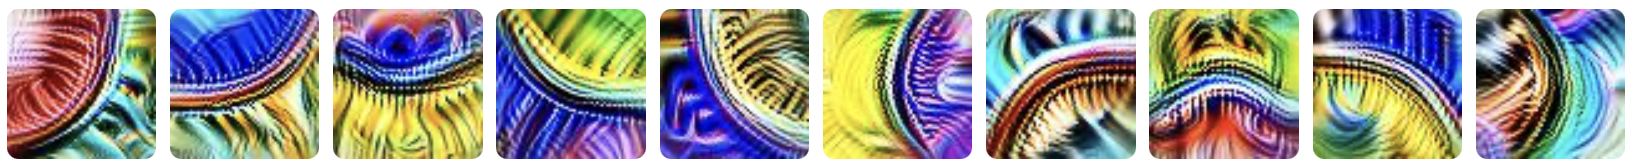
\includegraphics[width=1\linewidth]{images/curve_detector_3b379.png}
        \caption{}
        \label{fig:Ng1} 
    \end{subfigure}
    \medskip
    \begin{subfigure}[b]{0.75\textwidth}
        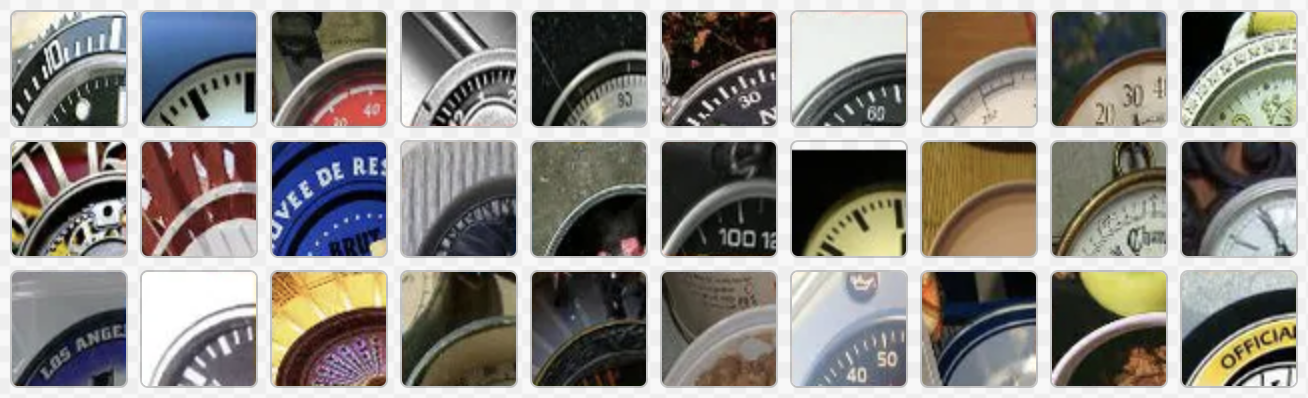
\includegraphics[width=1\linewidth]{images/dataset_samples.png}
        \caption{}
        \label{fig:Ng2}
    \end{subfigure}
    \caption{Wizualizacja neuronów zidentyfikowanych jako detektory krzywizn (a) oraz przykładowe obrazy ze zbioru danych (b) aktywujące te neurony w sieci \textit{InceptionV1}. Źródło: \cite{cammarata_2020_curve_detectors}, materiał udostępniony na licencji CC-BY 4.0.}
    \label{fig:curve_detector}
\end{figure}
\newline
Poza samą identyfikacją i weryfikacją selektywności neuronu, artykuł \textit{Zoom In} pokazuje również, w jaki sposób detektor ten jest zbudowany: analizując wagi łączące go z rodziną wcześniejszych detektorów linii o różnych orientacjach w poprzedniej warstwie, autorzy odczytują wprost z sieci algorytm detekcji krzywizny -- neuron sumuje pobudzenia od linii zorientowanych zgodnie z daną krzywizną i jednocześnie tłumi pobudzenia od linii o przeciwnej orientacji. \newline
\begin{figure}[h]
    \centering
    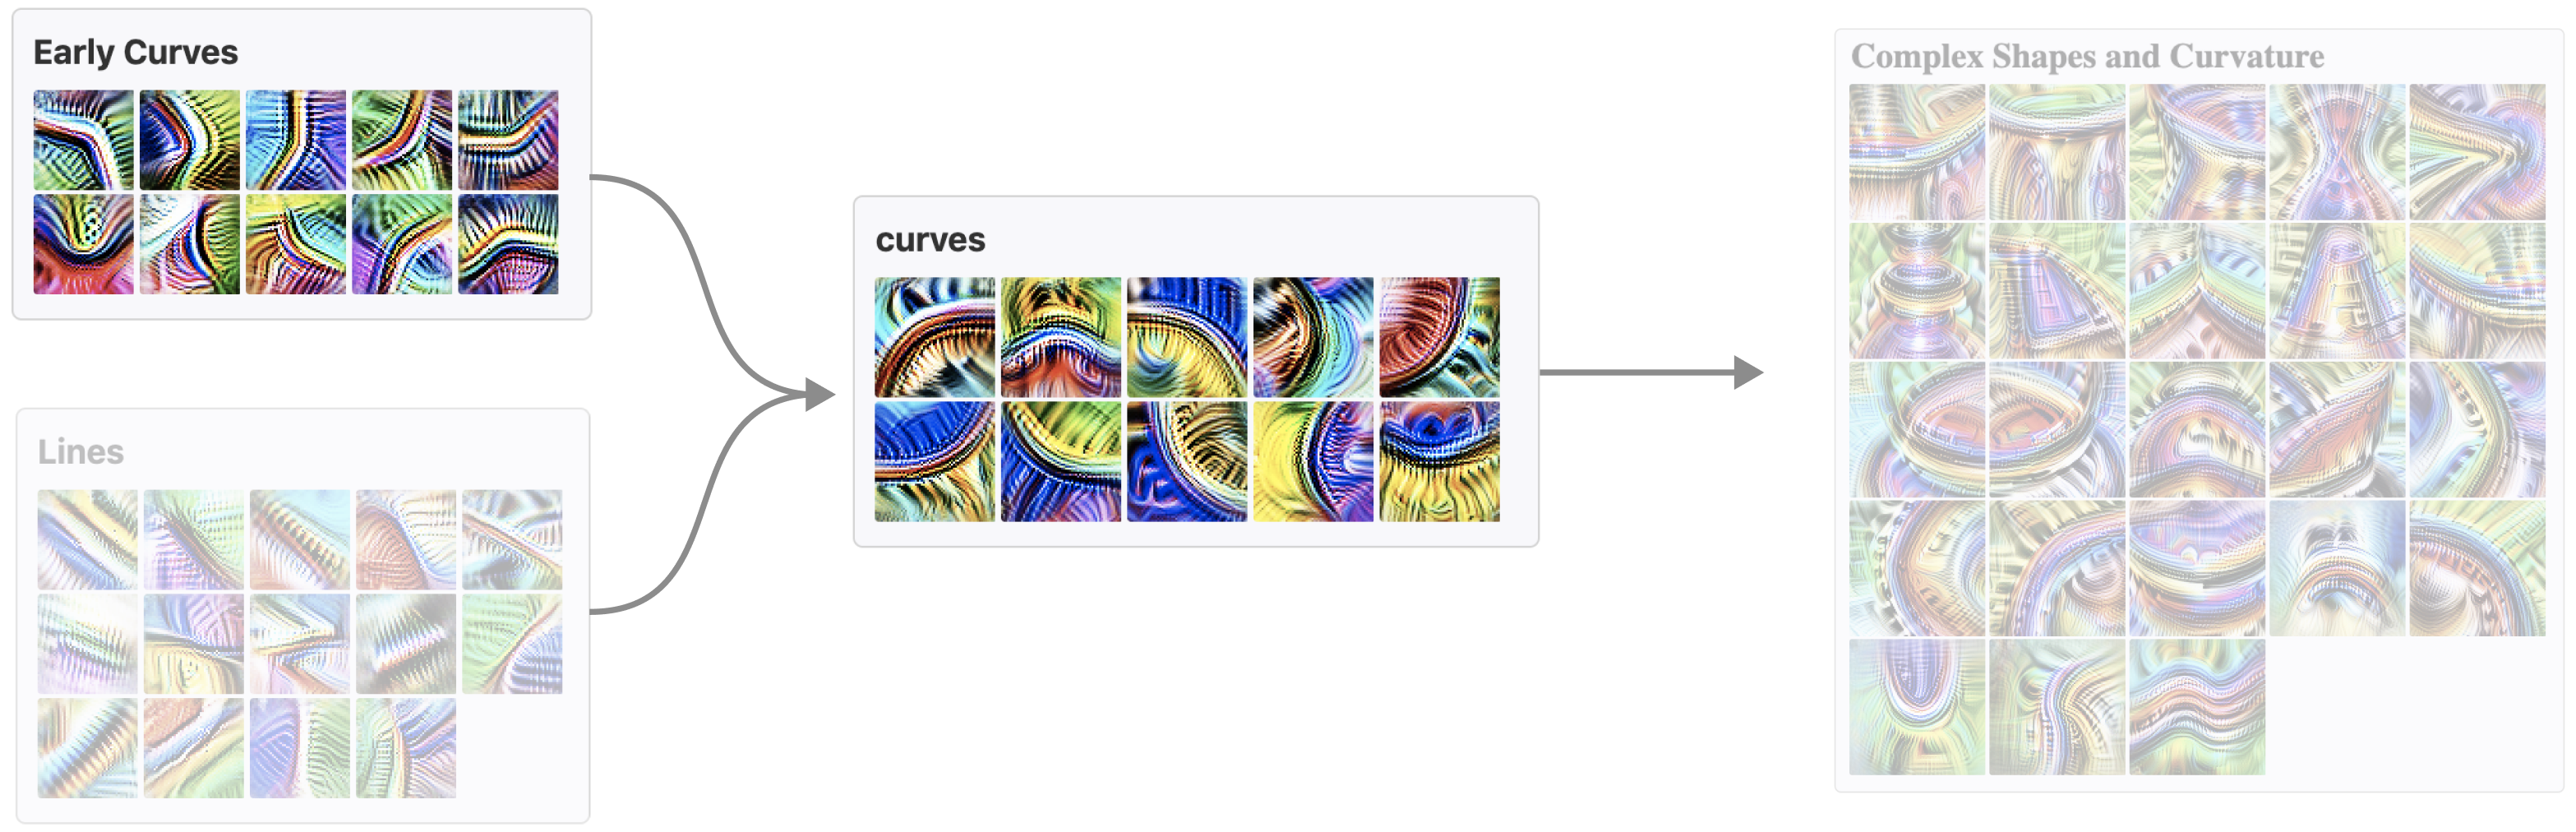
\includegraphics[width=1\textwidth]{images/curve_detector_circuit.png}
    \caption{Diagram wag ilustrujący obwód budujący detektory krzywizn z ważonej kombinacji wcześniejszych detektorów linii o różnych orientacjach. Źródło: \cite{olah_2020_zoom_in_circuits}, materiał udostępniony na licencji CC-BY 4.0.}
    \label{fig:curve_circuit_diagram}
\end{figure}
\newline
%Wizualizacja wag jako alternatywa dla analizy aktywacji - Visualizing Weights (Voss i in., 2021) -> kontekstualizacja, expanded weights, faktoryzacja (NMF) -> bezpośrednie powiązanie z planowaną analizą macierzy wag MLP (rozdz. 4) \newline -- obecnie poza zakresem pracy
Wszystkie omówione w tym podrozdziale prace -- od \textit{Feature Visualization}, przez \textit{Building Blocks of Interpretability} i \textit{Zoom In}, po \textit{Curve Detectors} oraz \textit{Visualizing Weights} -- łączy jedno istotne ograniczenie: cały program badawczy circuits rozwijany był niemal wyłącznie na sieciach konwolucyjnych przetwarzających obraz, a w większości przypadków na jednym, konkretnym, w pełni prześwietlonym modelu -- \textit{InceptionV1}. Podstawowe jednostki analizy -- krawędzie, linie, krzywizny, tekstury -- są więc z natury wizualne, a badane \enquote{fakty o świecie} sprowadzają się w praktyce do niskopoziomowych cech geometrycznych obrazu, nie do wiedzy faktograficznej czy relacji semantycznych, które stanowią przedmiot niniejszej pracy. Transfer tego programu badawczego na grunt architektury transformer i modeli językowych nie był przy tym automatyczny -- wymagał sformułowania nowego aparatu pojęciowego, dostosowanego do specyfiki strumienia rezydualnego, mechanizmu uwagi oraz warstw MLP pełniących funkcję pamięci klucz-wartość \cite{geva_2021_transformer_feedforward_key_value_memories}. Kontynuacją tego kierunku, prowadzoną w dużej mierze przez tych samych badaczy już w strukturach nowo powstałego \textit{Anthropic}, jest \textit{A Mathematical Framework for Transformer Circuits} \cite{elhage_2021_mathematical_framework_transformer_circuits}, formalizujący pojęcia obwodu i strumienia rezydualnego w kontekście transformerów -- oraz, opisany w dalszej części niniejszego rozdziału, problem superpozycji, wynikający bezpośrednio z napięcia zasygnalizowanego już w \textit{Zoom In}. Sposób, w jaki idee wypracowane na gruncie wizji komputerowej -- lokalizacja pojedynczej, dobrze scharakteryzowanej jednostki obliczeniowej oraz rekonstrukcja łączących je obwodów -- dają się przenieść na grunt wiedzy faktograficznej reprezentowanej przez modele językowe, jest tematem dalszego podrozdziału \ref{sec:interpretowalnosc_modeli_jezykowych}. \newline


\section{Architektura transformer}
\label{sec:architektura_transformer}
%TODO: może warto wyjaśnić czym jest atencja i wrzucić jakiś prosty matematyczny wzór albo schemat pokazujący jak działa (co jest mnożone przez co)
Architektura transformer, będąca dziś fundamentem niemal wszystkich dużych modeli językowych, została wprowadzona w pracy \textit{Attention Is All You Need} \cite{vaswani_2017_attention_is_all_you_need}, pierwotnie jako rozwiązanie zadania tłumaczenia maszynowego oparte na strukturze enkoder-dekoder. Podstawowym elementem tej architektury jest blok transformera, złożony z dwóch podwarstw. Ponieważ mechanizm uwagi sam w sobie jest niewrażliwy na kolejność tokenów w sekwencji, wejściowe osadzenia (ang. \textit{embedding}) tokenów są najpierw wzbogacane o kodowanie pozycyjne (w oryginalnej pracy -- sinusoidalne), niosące informację o miejscu tokenu w sekwencji. Pierwszą podwarstwą jest wielogłowy mechanizm samo-uwagi (ang. \textit{multi-head self-attention}), pozwalający każdej pozycji w sekwencji ważyć i agregować informacje pochodzące z pozostałych pozycji, przy czym równoległe działanie wielu głów uwagi umożliwia jednoczesne wychwytywanie różnych typów zależności między tokenami. Drugą podwarstwą jest warstwa feed-forward (MLP) -- dwie transformacje liniowe rozdzielone nieliniowością, stosowane niezależnie i identycznie do każdej pozycji z osobna. Obie podwarstwy opatrzone są połączeniami rezydualnymi, których koncepcja została zapożyczona z wcześniejszych prac nad głębokimi sieciami konwolucyjnymi \cite{he_2015_deep_residual_learning}, oraz normalizacją warstwową \cite{ba_2016_layer_normalization}, stabilizującą trening bardzo głębokich stosów takich bloków. Ten schemat, powielony wielokrotnie w głąb sieci, stanowi wspólny szkielet terminologiczny dla całej dalszej części niniejszego rozdziału. Schemat architektury przedstawiony został na rysunku \ref{fig:transofrmer_architecture}. \newline
\begin{figure}[h]
    \centering
    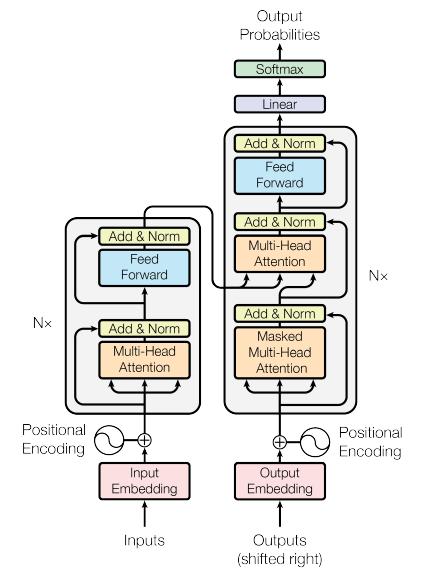
\includegraphics[width=0.5\textwidth]{images/transformer_architecture.png}
    \caption{Architektura modelu transformera zaprezentowana w pracy \textit{Attention Is All You Need} \cite{vaswani_2017_attention_is_all_you_need}. Przedstawia opisane wyżej podwarstwy mechanizmu uwagi oraz MLP wraz z połączeniami rezydualnymi połączone w bloki.}
    \label{fig:transofrmer_architecture}
\end{figure} % TODO: rozpikselizowany obraz
\newline
Choć sama architektura opisana przez Vaswaniego i in. wprowadza połączenia rezydualne jako techniczny środek ułatwiający propagację gradientu w głębokich sieciach, dopiero praca \textit{A Mathematical Framework for Transformer Circuits} \cite{elhage_2021_mathematical_framework_transformer_circuits} (omówiona szerzej w podrozdziale \ref{sec:interpretowalnosc_modeli_jezykowych}) opisuje ten mechanizm w kategorii możliwego do interpretowania, wprowadzając pojęcie strumienia rezydualnego (ang. \textit{residual stream}). Zgodnie z tym ujęciem, połączenia rezydualne można traktować jako wspólną \enquote{magistralę} informacyjną, przebiegającą przez cały model -- każda kolejna podwarstwa, zarówno attention, jak i MLP, odczytuje z niej swój stan wejściowy, wykonuje właściwe obliczenie, po czym addytywnie dopisuje wynik z powrotem do strumienia, nigdy go nie nadpisując. W konsekwencji stan strumienia w danej pozycji sekwencji jest sumą wkładów wszystkich poprzedzających go warstw, a każda kolejna warstwa ma pełny dostęp do wszystkiego, co zostało zapisane wcześniej. Istotnym ograniczeniem tego mechanizmu jest jednak niska, stała wymiarowość samego strumienia względem potencjalnie znacznie większej liczby komponentów, które chciałyby z niego korzystać jednocześnie -- warstwy muszą więc konkurować o ograniczoną przestrzeń kierunków, w których mogą zapisywać swoje wyniki. Ten problem strukturalnego \enquote{wąskiego gardła} stanowi bezpośredni punkt wyjścia do omawianego w dalszej części rozdziału zjawiska superpozycji. \newline
O ile poprzedni akapit opisuje strumień rezydualny jako wspólną magistralę, o tyle mechanizm uwagi i warstwa MLP pełnią w niej odmienne funkcje. Głowy uwagi przenoszą informację między pozycjami w sekwencji -- pozwalają danej pozycji \enquote{spojrzeć} na inne tokeny i skopiować lub zagregować niesione przez nie informacje z powrotem do strumienia rezydualnego we własnej pozycji. MLP natomiast operuje wyłącznie lokalnie, przetwarzając zawartość strumienia w obrębie pojedynczej pozycji, bez dostępu do pozostałych tokenów sekwencji. Najpełniej zinżynierowanym przykładem obwodu zbudowanego z tego pierwszego mechanizmu są tzw. \textit{induction heads}, opisane w pracy \textit{In-context Learning and Induction Heads} \cite{olsson_2022_induction_heads}. Autorzy identyfikują parę współpracujących głów uwagi rozłożonych w różnych warstwach modelu: głowę poprzedniego tokenu (ang. \textit{previous-token head}), zapisującą do strumienia rezydualnego informację o tokenie poprzedzającym daną pozycję, oraz właściwą głowę indukcyjną, która -- korzystając z tego zapisu za pośrednictwem tej samej magistrali strumienia rezydualnego -- przeszukuje wcześniejszy kontekst w poszukiwaniu poprzedniego wystąpienia bieżącego tokenu i kopiuje token, który wówczas po nim nastąpił, realizując w ten sposób prosty wzorzec dopasowania sekwencji [A][B]...[A]$\rightarrow$[B]. Jest to bezpośredni analog detektora krzywizny omówionego w podrozdziale \ref{sec:podejscie_obwodowe} -- pojedynczy obwód, osadzony w architekturze transformera i operujący na tokenach języka zamiast na pikselach obrazu, stanowiący pierwszy dowód na to, że program badawczy circuits daje się skutecznie przenieść z sieci wizyjnych na modele językowe. 
% MLP, w przeciwieństwie do tego mechanizmu opartego na przenoszeniu informacji, jest naturalnym kandydatem na miejsce jej przechowywania -- hipoteza ta, wraz z uzasadniającą ją interpretacją warstw MLP jako pamięci klucz-wartość, zostanie szerzej omówiona w podrozdziale \ref{sec:lokalizacja_wiedzy}. 
\newline
Oryginalna architektura opisana przez Vaswaniego i in. została zaprojektowana jako model enkoder-dekoder, w którym enkoder przetwarza całą sekwencję wejściową jednocześnie, a dekoder -- korzystając dodatkowo z mechanizmu \textit{cross-attention} czerpiącego z wyjścia enkodera -- generuje sekwencję wyjściową token po tokenie. Modele językowe typu GPT (ang. \textit{decoder-only}), zapoczątkowane pracą \textit{Improving Language Understanding by Generative Pre-Training} \cite{radford_2018_improving_language_understanding} i rozwinięte w \textit{Language Models are Unsupervised Multitask Learners} \cite{radford_2019_language_models_unsupervised_multitask_learners}, upraszczają ten schemat, odrzucając enkoder oraz cross-attention i pozostawiając wyłącznie stos bloków dekodera. Kluczową modyfikacją jest przy tym zastosowanie zamaskowanego (przyczynowego, ang. \textit{causal}) self-attention -- każda pozycja w sekwencji może uwzględniać w obliczeniu uwagi wyłącznie tokeny ją poprzedzające, nigdy przyszłe. Ograniczenie to sprawia, że model można trenować i wykorzystywać w sposób autoregresywny: przewidując kolejny token wyłącznie na podstawie tokenów dotychczas wygenerowanych. O ile praca Radforda i in. z 2018 roku traktuje generatywny pretrening przede wszystkim jako etap wstępny poprzedzający dostrajanie pod konkretne zadanie, o tyle \textit{GPT-2} \cite{radford_2019_language_models_unsupervised_multitask_learners} pokazuje, że sam czysty pretrening języka naturalnego, bez żadnego dostrajania zadaniowego, prowadzi do modelu zdolnego generalizować do wielu zadań jednocześnie -- ugruntowując tym samym architekturę dekoderową jako samodzielny, dominujący dziś paradygmat budowy modeli językowych. To właśnie ten wariant architektoniczny wybrano jako podstawę eksperymentów niniejszej pracy, zgodnie z założeniami przedstawionymi w podrozdziale \ref{sec:cele}. \newline

\section{Interpretowalność modeli językowych}
\label{sec:interpretowalnosc_modeli_jezykowych}
Podrozdział \ref{sec:architektura_transformer} przedstawił architekturę transformer w ujęciu czysto strukturalnym -- jako następujące po sobie bloki uwagi i MLP, komunikujące się za pośrednictwem strumienia rezydualnego. Sam ten opis nie rozstrzyga jednak, w jaki sposób można zbadać, co dzieje się wewnątrz tak zdefiniowanej struktury podczas przetwarzania konkretnego tekstu. Pytanie to, postawione ogólnie w podrozdziale \ref{sec:interpretowalnosc_sieci_neuronowych}, powraca tutaj w wersji dostosowanej do modeli językowych, wzdłuż tego samego podziału na podejście reprezentacyjne i mechanistyczne. Pierwsze z nich pyta, jaka informacja jest w danym momencie zakodowana w strumieniu rezydualnym -- realizują je metody sondujące (podrozdział \ref{sec:probing}) oraz logit lens (podrozdział \ref{sec:logit_lens}), operujące wyłącznie na aktywacjach modelu. Drugie, zgodnie z duchem podejścia obwodowego z podrozdziału \ref{sec:podejscie_obwodowe}, pyta wprost, jaki mechanizm zapisany w wagach modelu tę informację wytwarza -- odpowiada na to matematyczny opis obwodów transformera (podrozdział \ref{sec:framework_obwodow}), rozwijający program \textit{circuits} na grunt architektury opisanej w poprzednim podrozdziale. Obie tradycje dostarczają narzędzi wykorzystanych w dalszej części pracy, w tym w potoku analitycznym opisanym w rozdziale 3. \newline
\subsection{Metody sondujące (ang. \textit{probing classifiers})}
\label{sec:probing}
Najprostszym sposobem zadania pytania, jaka informacja o przetwarzanym tekście jest zakodowana w reprezentacji danej warstwy, jest pominięcie mechanizmu jej powstawania i sprawdzenie jedynie, czy informacja ta daje się z tej reprezentacji odczytać. Metodę tę, nazywaną sondowaniem (ang. \textit{probing}), sformalizowali Guillaume Alain i Yoshua Bengio \cite{alain_2016_understanding_intermediate_layers_using_linear_classifier_probes}: polega ona na zamrożeniu wag badanej sieci i wytrenowaniu dodatkowego, zwykle liniowego klasyfikatora (tzw. sondy, ang. \textit{probe}) na aktywacjach wybranej warstwy, mającego przewidzieć z góry zdefiniowaną własność przetwarzanych danych. Wysoka skuteczność takiej sondy świadczy o tym, że badana własność jest w danej warstwie reprezentowana w sposób liniowo dekodowalny -- niezależnie od tego, jaki mechanizm doprowadził do jej zakodowania. \newline
Metodę tę zastosowali do modeli językowych Ian Tenney i współpracownicy w pracy \textit{BERT Rediscovers the Classical NLP Pipeline} \cite{tenney_2019_bert_rediscovers_classical_nlp_pipeline}, trenując sondy do klasycznych zadań lingwistycznych -- znakowania części mowy, analizy składniowej, przypisywania ról semantycznych oraz rozwiązywania koreferencji -- na zamrożonych reprezentacjach kolejnych warstw modelu BERT. Autorzy pokazali, że zadania te dają się uporządkować zgodnie z rosnącą głębokością sieci w kolejności odpowiadającej klasycznemu potokowi przetwarzania języka naturalnego -- zadania powierzchniowe są najlepiej dekodowalne z warstw wcześniejszych, a zadania wymagające przetwarzania bardziej abstrakcyjnego z warstw głębszych. Wynik ten stanowi językowy odpowiednik hierarchii cech zaobserwowanej wcześniej w sieciach konwolucyjnych (podrozdział \ref{sec:wczesne_prace_wizualizacja}) -- od krawędzi po całe obiekty -- i dostarczył jednego z pierwszych empirycznych dowodów na to, że głębokość sieci językowej koreluje z poziomem abstrakcji przetwarzanej informacji. \newline
Warto przy tym zaznaczyć, że wyniki Tenney i współpracowników uzyskano na modelu BERT, a więc architekturze enkoderowej, przetwarzającej sekwencję dwukierunkowo. Sama metoda sondująca jest jednak niezależna od architektury i w tej samej postaci daje się zastosować do modeli dekoderowych, takich jak model wykorzystany w niniejszej pracy (podrozdział \ref{sec:cele}).
\subsection{Logit lens}
\label{sec:logit_lens}
W odróżnieniu od metod sondujących, wymagających wytrenowania dodatkowego klasyfikatora na aktywacjach badanej warstwy, modele dekoderowe typu GPT dają możliwość odczytania stanu pośredniego strumienia rezydualnego bez żadnego dodatkowego treningu. Wynika to z samej konstrukcji tych modeli: ostateczny stan strumienia rezydualnego jest, po zastosowaniu normalizacji warstwowej (ang. \textit{layer normalization}), rzutowany na przestrzeń słownika za pomocą macierzy unembeddingu, dającej w wyniku rozkład prawdopodobieństwa nad kolejnym tokenem. Technika logit lens, powstała w formie nieformalnego wpisu na forum \textit{LessWrong} \cite{nostalgebraist_2020_logit_lens}, wykorzystuje ten sam mechanizm przedwcześnie -- rzutuje na przestrzeń słownika stan strumienia rezydualnego odczytany z warstwy pośredniej, tak jakby był on już stanem końcowym. Powtarzając tę operację dla kolejnych warstw modelu, można prześledzić, jak rozkład przewidywanego tokenu ewoluuje wraz z głębokością sieci -- od niespecyficznych, często wysokoczęstotliwościowych przewidywań we wczesnych warstwach, po coraz bardziej trafną i ostateczną predykcję w warstwach końcowych. \newline
Metoda ta przyjęła się jako standardowe narzędzie eksploracyjne w badaniach nad interpretowalnością modeli językowych, ze względu na jej prostotę i brak kosztu obliczeniowego związanego z treningiem. Warto przy tym zaznaczyć, że technika ta niejawnie zakłada, iż reprezentacje pośrednie warstw są wyrażone w tej samej bazie co reprezentacja warstwy końcowej. Założenie to jest jednak jedynie przybliżeniem, przez co zwłaszcza w warstwach początkowych rzutowane rozkłady bywają niespójne i trudne do zinterpretowania jako sensowne predykcje kolejnego tokenu. Im głębsza jednak warstwa, z której pochodzi rzutowany stan, tym rzutowana predykcja staje się zwykle coraz bardziej spójna i zbliżona do finalnego wyniku modelu.

\subsection{Matematyczny opis obwodów transformera}
\label{sec:framework_obwodow}
%TODO: czy nie trzeba sprecyzować czemu ta metoda jest opisywana obok probing i logit lens? Tutaj chyba słabe jest to wytłumaczenie
O ile metody sondujące i logit lens analizują stan strumienia rezydualnego wywołany przez konkretny tekst wejściowy, o tyle praca \textit{A Mathematical Framework for Transformer Circuits} \cite{elhage_2021_mathematical_framework_transformer_circuits} proponuje podejście działające wyłącznie na poziomie wag modelu. Punktem wyjścia jest obserwacja, że skoro każda podwarstwa komunikuje się ze strumieniem rezydualnym (podrozdział \ref{sec:architektura_transformer}) wyłącznie za pośrednictwem operacji liniowych, to nawet odległe od siebie warstwy można opisać efektywną zależnością liniową, wyliczoną wprost z iloczynu ich macierzy wag -- bez uruchamiania modelu na jakichkolwiek danych. Na tej podstawie autorzy rozkładają mechanizm uwagi na dwa niezależne obwody: decydujący o tym, które pozycje w sekwencji są brane pod uwagę, oraz decydujący, jaka informacja zostaje na tej podstawie skopiowana z powrotem do strumienia. Takie podejście pozwoliło formalnie wyjaśnić działanie induction heads, opisanych w podrozdziale \ref{sec:architektura_transformer} \cite{olsson_2022_induction_heads}, jako przykład współpracy dwóch głów uwagi rozłożonych w różnych warstwach. \newline
Analiza ta prowadzi jednak autorów do istotnego zastrzeżenia wobec własnej metody: ze względu na liniową, addytywną strukturę strumienia rezydualnego, nie posiada on żadnej wyróżnionej, \enquote{uprzywilejowanej bazy} (ang. \textit{privileged basis}) -- nic nie gwarantuje, że pojedynczy neuron czy pojedynczy wymiar strumienia odpowiada jednemu, czytelnemu konceptowi. Co więcej, liczba komponentów obliczeniowych (neuronów warstw MLP, wymiarów wyniku głów uwagi) konkurujących o miejsce w strumieniu znacząco przewyższa jego wymiarowość, zmuszając je -- jak to określają sami autorzy -- do komunikowania się w superpozycji. Zjawisko to, jedynie zasygnalizowane w opisywanej pracy, stanowi przedmiot kolejnego podrozdziału.

\section{Problem superpozycji i geneza rzadkich autoenkoderów}
\label{sec:superpozycja}
Podrozdział \ref{sec:framework_obwodow} zasygnalizował zjawisko superpozycji, nie wyjaśniając jednak wprost, na czym ono polega -- ograniczona, stała wymiarowość strumienia rezydualnego, zestawiona z brakiem jego uprzywilejowanej bazy, zmusza konkurujące o miejsce w nim komponenty obliczeniowe do dzielenia się tymi samymi kierunkami. Niniejszy podrozdział wyjaśnia mechanikę tego zjawiska na przykładzie modelu roboczego zaproponowanego przez zespół Anthropic, po czym omawia jego konsekwencje dla interpretacji pojedynczych jednostek sieci (podrozdział \ref{sec:polisemantycznosc}) oraz sposób, w jaki próba jego odwrócenia doprowadziła do sformułowania hipotezy słownikowej -- bezpośredniego pomostu do rzadkich autoenkoderów, będących przedmiotem dalszej części niniejszego rozdziału (podrozdział \ref{sec:hipoteza_slownikowa}).
\subsection{Zjawisko superpozycji}
\label{sec:zjawisko_superpozycji}
Punktem wyjścia dla zrozumienia superpozycji jest tzw. hipoteza reprezentacji liniowej (ang. \textit{linear representation hypothesis}), zgodnie z którą pojedyncza cecha (ang. \textit{feature}) -- rozumiana jako odrębny, interpretowalny koncept reprezentowany przez sieć -- odpowiada nie pojedynczemu neuronowi, lecz pewnemu kierunkowi w wielowymiarowej przestrzeni aktywacji. Założenie to obecne już w metodach sondujących i w programie circuits omówionych we wcześniejszych podrozdziałach, prowadzi do pytania, ile takich kierunków sieć jest w stanie jednocześnie utrzymać, skoro liczba potencjalnie istotnych konceptów świata rzeczywistego, które model powinien rozróżniać, znacząco przewyższa liczbę neuronów dostępnych w pojedynczej warstwie. \newline
Odpowiedzi na to pytanie udzielają Nelson Elhage i współpracownicy z Anthropic w pracy \textit{Toy Models of Superposition} \cite{elhage_2022_toy_models_of_superposition}, konstruując silnie uproszczony model, w którym zjawisko to można badać w pełni kontrolowanych warunkach: wektor cech o wymiarowości znacząco przewyższającej wymiarowość warstwy ukrytej jest do niej liniowo rzutowany, a następnie odtwarzany z powrotem za pomocą tej samej macierzy wag i nieliniowości ReLU. Każda cecha wejściowa charakteryzuje się rzadkością (ang. \textit{sparsity}) -- prawdopodobieństwem, że w danej chwili przyjmuje wartość zerową -- oraz ważnością (ang. \textit{importance}), określającą, jak silnie błąd jej rekonstrukcji obciąża łączną funkcję straty. \newline
Autorzy pokazują, że zachowanie modelu silnie zależy od rzadkości reprezentowanych cech. Gdy cechy są gęste, a przestrzeń ukryta nie wystarcza do zakodowania wszystkich z nich, model reprezentuje jedynie tyle cech, ile ma do dyspozycji wymiarów, pomijając resztę. W miarę wzrostu rzadkości model zaczyna jednak reprezentować więcej cech niż posiada wymiarów, przypisując im nieortogonalne, nakładające się na siebie kierunki -- godząc się na pewną wzajemną interferencję między nimi w zamian za zwiększoną pojemność reprezentacyjną. Właśnie to zjawisko autorzy nazywają superpozycją, a umożliwia je zastosowana w kroku rekonstrukcji nieliniowość ReLU, tłumiąca drobną interferencję pochodzącą od nieaktywnych w danej chwili cech. \newline
Zjawisko to ma bezpośrednie konsekwencje dla sposobu, w jaki należy interpretować pojedyncze jednostki sieci -- zagadnieniu temu poświęcony jest kolejny podrozdział.
\subsection{Polisemantyczność}
\label{sec:polisemantycznosc}
Zjawisko superpozycji opisane w poprzednim podrozdziale dostarcza mechanistycznego wyjaśnienia obserwacji poczynionej już w podrozdziale \ref{sec:podejscie_obwodowe} -- autorzy \textit{Zoom In} \cite{olah_2020_zoom_in_circuits} zauważyli, że część neuronów sieci \textit{InceptionV1} jest polisemantyczna, tzn. aktywuje się w odpowiedzi na kilka odrębnych, niepowiązanych ze sobą pojęć jednocześnie \cite{olah_2020_zoom_in_circuits}. Pracy \textit{Toy Models of Superposition} dokładniej skupia się na tym zjawisku: skoro sieć reprezentuje więcej cech niż posiada wymiarów, przypisując im nieortogonalne, nakładające się kierunki, to pojedynczy neuron z konieczności bierze udział w kodowaniu wielu z nich naraz. Polisemantyczność jest więc oczekiwaną konsekwencją superpozycji przy ograniczonej wymiarowości sieci. \newline
Wniosek ten podważa założenie leżące u podstaw większości metod omówionych w podrozdziałach \ref{sec:wczesne_prace_wizualizacja} i \ref{sec:podejscie_obwodowe} -- że pojedyncza, dobrze scharakteryzowana jednostka sieci (neuron, kanał) stanowi naturalną, monosemantyczną jednostkę analizy. Zarówno maksymalizacja aktywacji \cite{olah_2017_feature_visualization}, jak i studium przypadku pojedynczego neuronu w \textit{Curve Detectors} \cite{cammarata_2020_curve_detectors} zakładają, że wyjaśnienie znaczenia jednego neuronu jest zadaniem dobrze postawionym. W obecności superpozycji założenie to jest jednak spełnione jedynie częściowo -- część neuronów faktycznie odpowiada w przybliżeniu jednemu konceptowi, inne zaś są superpozycją wielu niepowiązanych ze sobą cech, co czyni ich bezpośrednią interpretację niejednoznaczną. \newline
Powyższe ograniczenie rodzi pytanie, czy możliwe jest odzyskanie z superpozycji jednostek bliższych rzeczywistym, monosemantycznym cechom, zamiast poprzestawać na analizie pojedynczych, potencjalnie polisemantycznych neuronów. Remedium na ten problem, wywodzące się z tzw. hipotezy słownikowej, jest omówione w kolejnym podrozdziale.
\subsection{Hipoteza słownikowa}
\label{sec:hipoteza_slownikowa}
Skoro, jak pokazano w podrozdziale \ref{sec:zjawisko_superpozycji}, sieć koduje rzadkie cechy jako nadpełny (ang. \textit{overcomplete}), nakładający się na siebie zestaw kierunków w przestrzeni aktywacji, to zadanie odzyskania tych cech można sformułować jako problem odwrotny: obserwowany wektor aktywacji jest rzadką kombinacją liniową nieznanych, rzeczywistych kierunków bazowych, a celem jest odtworzenie zarówno tych kierunków, jak i rzadkich współczynników, z jakich każda konkretna aktywacja jest złożona. Sformułowany w ten sposób problem odpowiada dokładnie klasycznemu zagadnieniu rzadkiego uczenia się słownika (ang. \textit{sparse dictionary learning}), znanego wcześniej z zastosowań poza dziedziną modeli językowych. \newline
Zastosowanie tego podejścia do aktywacji sieci neuronowych zaproponowali Lee Sharkey, Dan Braun i Beren Millidge w raporcie badawczym \textit{Taking Features Out of Superposition With Sparse Autoencoders} \cite{sharkey_2022_taking_features_out_of_superposition}, bezpośrednio nawiązującym do wyników opisanych w \textit{Toy Models of Superposition}. Autorzy proponują wytrenowanie rzadkiego autoenkodera (ang. \textit{Sparse Autoencoder}, SAE) -- sieci złożonej z enkodera rzutującego aktywacje badanego modelu w znacznie szerszą, nadpełną przestrzeń ukrytą, oraz dekodera odtwarzającego z niej oryginalną aktywację jako jej liniową kombinację. Kara za brak rzadkości, nałożona na aktywacje warstwy ukrytej, wymusza, by w rekonstrukcji każdej pojedynczej aktywacji brała udział jedynie niewielka liczba kierunków tego nadpełnego słownika -- w zamierzeniu odpowiadających pojedynczym, monosemantycznym cechom, zamiast ich superpozycji. \newline
Propozycja ta, sformułowana jeszcze jako wstępny raport badawczy i zweryfikowana wyłącznie na niewielkich modelach, otworzyła jednak drogę do serii prac stosujących rzadkie autoenkodery bezpośrednio do modeli językowych -- ich przegląd jest przedmiotem kolejnego podrozdziału.

\section{Rzadkie autoenkodery (SAE) jako narzędzie dekompozycji reprezentacji}
\label{sec:sae_dekompozycja}
Hipoteza słownikowa omówiona w poprzednim podrozdziale (\ref{sec:hipoteza_slownikowa}) wprowadzała koncepcję rzadkiego autoenkodera zweryfikowaną na modelu roboczym -- pojedynczym, jednowarstwowym transformerze, dobranym tak, by ułatwić kontrolowaną analizę. Otwarte pozostawało więc pytanie, czy metoda ta przenosi się na modele o istotnie większej skali oraz czy wyodrębnione w ten sposób kierunki rzeczywiście odpowiadają czytelnym, monosemantycznym konceptom. Niniejszy podrozdział prześledzi, jak na te pytania odpowiedziała kolejna fala prac -- począwszy od pierwszej walidacji podejścia na realnych modelach językowych, przez rozwinięcia architektoniczne, aż po metodykę przyjętą w niniejszej pracy.

\subsection{Pierwsze zastosowania SAE na aktywacjach modeli językowych}
\label{sec:sae_pierwsze_prace}
Jesienią 2023 roku, niezależnie od siebie i w odstępie zaledwie kilku tygodni, opublikowane zostały dwie prace \cite{cunningham_2023_sparse_autoencoders_highly_interpretable_features, bricken_2023_towards_monosemanticity_dictionary_learning}, które po raz pierwszy zastosowały rzadkie autoenkodery do aktywacji rzeczywistych modeli językowych. Dwa niezależne zespoły, stosując odmienne modele i protokoły ewaluacji, doszły do zgodnego wniosku, że rzadkie autoenkodery rzeczywiście dekomponują aktywacje na kierunki bardziej interpretowalne niż kierunki wskazywane przez metody alternatywne. \newline
Hoagy Cunningham i współpracownicy w pracy \textit{Sparse Autoencoders Find Highly Interpretable Features in Language Models} \cite{cunningham_2023_sparse_autoencoders_highly_interpretable_features} skupili się przede wszystkim na ilościowym udowodnieniu tej przewagi. Wyodrębnione przez SAE kierunki porównali z kierunkami wskazywanymi przez metody bazowe -- analizę głównych składowych (ang. \textit{Principal Component Analysis}, PCA), analizę składowych niezależnych (ang. \textit{Independent Component Analysis}, ICA) oraz surowe kierunki odpowiadające pojedynczym neuronom. Do oceny interpretowalności każdego kierunku zastosowali zautomatyzowaną metodę, wywodzącą się z wcześniejszych prac nad wyjaśnianiem pojedynczych neuronów: dla danej cechy generowany jest opis słowny na podstawie fragmentów tekstu najsilniej ją aktywujących, a jakość tego opisu weryfikuje się, sprawdzając, na ile pozwala on przewidzieć aktywację cechy na nowym, niewidzianym wcześniej fragmencie tekstu. Zgodnie z tą metryką kierunki wskazywane przez SAE okazały się systematycznie bardziej interpretowalne niż kierunki wskazywane przez każdą z metod bazowych.
\begin{figure}[h]
    \centering
    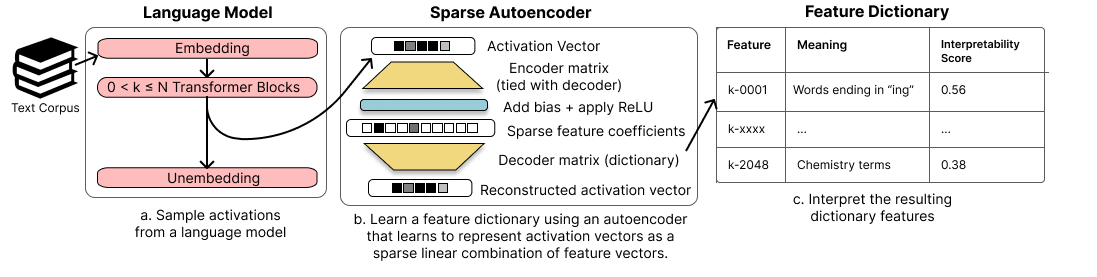
\includegraphics[width=\textwidth]{images/sae_training.png}
    \caption{Ogólny proces uczenia modelu autoenkodera stosowany w większości eksperymentów, a także zastosowany na potrzeby niniejszej pracy. Grafika pochodzi z pracy \textit{Sparse Autoencoders Find Highly Interpretable Features in Language Models} \cite{cunningham_2023_sparse_autoencoders_highly_interpretable_features}.}
    \label{fig:sae_training}
\end{figure}
\newline
Równolegle Trenton Bricken i współpracownicy z Anthropic opublikowali \textit{Towards Monosemanticity: Decomposing Language Models With Dictionary Learning} \cite{bricken_2023_towards_monosemanticity_dictionary_learning} -- pracę skupioną w mniejszym stopniu na porównaniu z metodami alternatywnymi, a w większym na dogłębnej analizie samego procesu treningu SAE i wypracowaniu metodyki jego oceny, która stała się później de facto standardem przyjmowanym przez kolejne prace omówione w dalszej części niniejszego rozdziału. Eksperymenty przeprowadzono na celowo bardzo małym modelu -- jednowarstwowym transformerze z warstwą MLP liczącą 512 neuronów -- co pozwoliło na wielokrotne powtórzenie treningu przy różnych wartościach hiperparametrów i rozmiarach słownika cech. Autorzy zdefiniowali dwie podstawowe, wzajemnie sprzeczne miary jakości dekompozycji: stratę rekonstrukcji (ang. \textit{reconstruction loss}), mierzącą, jak wiernie autoenkoder odtwarza oryginalną aktywację, oraz rzadkość $L0$, rozumianą jako średnią liczbę jednocześnie aktywnych cech przypadającą na pojedynczą aktywację wejściową. Zmniejszanie $L0$ zwykle pogarsza rekonstrukcję, co czyni dobór właściwego punktu na tym kompromisie centralnym zagadnieniem praktycznym przy treningu. \newline
Praca ta zidentyfikowała również dwa zjawiska, które muszą być brane pod uwagę przy każdym treningu SAE. Pierwszym są martwe cechy (ang. \textit{dead features}) -- kierunki słownika, które w trakcie treningu przestają się aktywować dla jakiegokolwiek fragmentu danych i nigdy nie powracają do użycia, efektywnie zmniejszając rzeczywistą pojemność autoenkodera poniżej nominalnego rozmiaru jego słownika. Drugim jest zjawisko rozszczepiania cech (ang. \textit{feature splitting}): w miarę zwiększania rozmiaru słownika pojedyncza, szeroka cecha wyodrębniona przy mniejszym słowniku rozszczepia się na kilka węższych, bardziej wyspecjalizowanych cech przy słowniku większym -- co sugeruje, że granice pomiędzy konceptami reprezentowanymi przez sieć nie są ustalone raz na zawsze, lecz zależą od rozdzielczości, z jaką próbujemy je odczytać.

\subsection{Sterowanie cechami (ang. \textit{feature steering})}
\label{sec:sae_feature_steering}
Metody omówione w poprzednim podrozdziale weryfikowały jakość dekompozycji SAE metrykami natury korelacyjnej -- zgodnością automatycznie wygenerowanego opisu cechy z tekstem ją aktywującym, stratą rekonstrukcji czy rzadkością $L0$. Żadna z nich nie odpowiada jednak wprost na pytanie, czy dana cecha rzeczywiście ma wpływ na zachowanie modelu, czy jedynie koreluje z pewnym wzorcem obecnym w danych wejściowych. Już Bricken i współpracownicy \cite{bricken_2023_towards_monosemanticity_dictionary_learning} zaproponowali prostą formę takiej weryfikacji: sztuczne wymuszenie ustalonej wartości aktywacji wybranej cechy podczas generowania tekstu (ang. \textit{feature steering}) i obserwację wynikającej z tego zmiany zachowania modelu. \newline
Templeton i współpracownicy \cite{templeton_scaling_monosemanticity} pokazali, że ta sama technika generalizuje się do modelu o skali produkcyjnej -- wzmacniając sztucznie aktywację pojedynczej cechy w modelu \textit{Claude 3 Sonnet}, uzyskali przewidywalną, spójną zmianę generowanego tekstu (najczęściej cytowanym przykładem jest cecha powiązana z mostem Golden Gate, której wymuszona aktywacja sprawiała, że model nawiązywał do mostu niezależnie od tematu rozmowy). Istotność tego wyniku nie leży jednak w samej anegdotyczności przykładu, lecz w tym, że stanowi on bezpośredni dowód na związek przyczynowy, między wyodrębnioną cechą a zachowaniem modelu -- odróżniając w ten sposób walidację SAE od walidacji metod atrybucyjnych opisanych w podrozdziale \ref{sec:wczesne_prace_wizualizacja}, które takiej przyczynowości wprost nie gwarantowały. Wzorzec ten -- lokalizacja cechy, a następnie jej przyczynowa weryfikacja poprzez interwencję -- zostanie wykorzystany również w metodyce walidacji przyjętej w niniejszej pracy. \newline
Mimo tych sukcesów, zarówno na małej, jak i produkcyjnej skali, sama architektura rzadkiego autoenkodera stosowana we wszystkich dotychczas omówionych pracach pozostawała niezmieniona od czasu \textit{Toy Models of Superposition} -- a wraz z nią nierozwiązany problem systematycznego zaniżania siły rekonstruowanych aktywacji, do którego odnosi się kolejny podrozdział.

\subsection{Warianty architektoniczne}
\label{sec:sae_warianty}
Wspólnym mianownikiem architektury SAE stosowanej we wszystkich dotychczas omówionych pracach był enkoder liniowy z nieliniowością ReLU, trenowany z karą $L1$ nałożoną na aktywacje warstwy ukrytej -- dokładnie taki, jaki zaproponowali Sharkey i współpracownicy w \cite{sharkey_2022_taking_features_out_of_superposition}. Kara $L1$, choć skuteczna w wymuszaniu rzadkości, wprowadza jednak systematyczne obciążenie zwane \textit{shrinkage}: ponieważ kara ta rośnie liniowo wraz z wielkością aktywacji niezależnie od tego, czy dana wielkość jest optymalna dla wiernej rekonstrukcji, optymalizacja premiuje zaniżanie aktywacji względem wartości, która najlepiej odtworzyłaby oryginalny sygnał. W efekcie nawet poprawnie zidentyfikowana, rzeczywiście aktywna cecha zostaje odtworzona z systematycznie zaniżoną siłą, co pogarsza jakość rekonstrukcji ponad to, czego wymagałaby sama rzadkość. \newline
Pierwszą próbą adresującą ten problem był \textit{Gated SAE}, zaproponowany przez Rajamanoharana i współpracowników \cite{rajamanoharan_2024a_gated_sparse_autoencoders}. Autorzy rozdzielili dwie decyzje, które w standardowym SAE podejmowane są łącznie przez tę samą nieliniowość: czy dana cecha powinna być aktywna, oraz jaką powinna mieć wielkość. Pierwszą decyzję podejmuje osobna gałąź bramkująca, karana za pomocą $L1$, drugą zaś -- gałąź odpowiedzialna wyłącznie za wielkość aktywacji, nieobjęta tą karą. Ponieważ \textit{shrinkage} wynikał właśnie z nałożenia kary $L1$ na wielkość aktywacji, jej przeniesienie na osobną, niepenalizowaną ścieżkę częściowo łagodzi to zjawisko, przy zachowaniu tego samego mechanizmu wymuszania rzadkości. \newline
Rozwiązanie bardziej radykalne zaproponowali Gao i współpracownicy w pracy \textit{Scaling and Evaluating Sparse Autoencoders} \cite{gao_2024_scaling_evaluating_sparse_autoencoders}, wprowadzając architekturę Top-K SAE. Zamiast karać wielkość aktywacji karą $L1$, autorzy usuwają ją całkowicie, zastępując wybór aktywnych cech twardym mechanizmem: dla każdej aktywacji wejściowej zachowywanych jest jedynie $k$ cech o największej sile pobudzenia, pozostałe zaś są zerowane. Rozwiązanie to eliminuje shrinkage u źródła -- skoro żadna kara nie jest nakładana na wielkość zachowanych aktywacji, rekonstrukcja nie jest już zniekształcana w stronę zaniżonych wartości -- a jednocześnie daje badaczowi bezpośrednią kontrolę nad rzadkością $L0$ poprzez sam dobór parametru $k$, bez potrzeby żmudnego strojenia współczynnika kary. Problem martwych cech, opisany już przez Brickena i współpracowników (podrozdział \ref{sec:sae_pierwsze_prace}), autorzy adresują dodatkową funkcją straty pomocniczej, wymuszającą, by nieaktywne cechy nadal otrzymywały sygnał gradientowy poprzez próbę odtworzenia błędu rekonstrukcji. Praca ta dostarcza również pierwszych praw skalowania dla SAE, analogicznych do praw skalowania znanych z treningu samych modeli językowych -- wiążących jakość rekonstrukcji z rozmiarem słownika cech i budżetem obliczeniowym przeznaczonym na trening. \newline
Ograniczeniem architektury Top-K jest jednak sam parametr $k$: liczba aktywnych cech jest identyczna dla każdej aktywacji wejściowej, niezależnie od tego, czy dany fragment tekstu wymaga do opisania kilku, czy kilkudziesięciu konceptów jednocześnie. Odpowiedzią na to ograniczenie jest JumpReLU SAE, zaproponowany przez Rajamanoharana i współpracowników \cite{rajamanoharan_2024b_jumprelu_sparse_autoencoders}. Zamiast globalnego, jednakowego dla wszystkich cech parametru $k$, każda cecha otrzymuje własny, uczony podczas treningu próg aktywacji: aktywacje poniżej progu są zerowane, powyżej -- przepuszczane bez zmian, a więc również bez towarzyszącego zjawisku shrinkage. Ponieważ funkcja progowa nie jest różniczkowalna, trening odbywa się z wykorzystaniem estymatorów prostoliniowych (ang. \textit{straight-through estimators}), przybliżających gradient w otoczeniu progu. Tak skonstruowany SAE pozwala na zmienną, zależną od wejścia liczbę aktywnych cech i -- według autorów -- osiąga najwyższą wierność rekonstrukcji przy zadanym poziomie rzadkości spośród porównywanych architektur, w tym Gated i Top-K SAE. \newline
Postęp architektoniczny opisany w niniejszym podrozdziale skutecznie ograniczył zjawisko shrinkage, nie rozstrzygnął jednak pytania bardziej fundamentalnego: czy wyodrębniony w ten sposób słownik cech jest jednoznacznie wyznaczony przez badany model, czy stanowi jedynie jedno z wielu równie uprawnionych rozwiązań tego samego zadania optymalizacyjnego. Paulo i Belrose \cite{paulo_2025_sae_trained_on_same_data_learn_different_features} pokazali, że SAE trenowane na tych samych aktywacjach tego samego modelu, różniące się wyłącznie ziarnem losowości użytym do inicjalizacji wag, wyodrębniają istotnie różne zestawy cech -- w jednym z badanych przypadków jedynie $30\%$ cech pokrywało się pomiędzy niezależnymi powtórzeniami treningu. Co więcej, autorzy zaobserwowali, że architektura Top-K, mimo przewagi pod względem wierności rekonstrukcji, wykazuje większą niestabilność międzyseedową niż klasyczny SAE trenowany z karą $L1$, nawet przy kontrolowanym poziomie rzadkości. Wniosek ten nakazuje ostrożność w interpretowaniu wyodrębnionych cech jako jednoznacznych, obiektywnie istniejących jednostek obliczeniowych modelu. \newline
Wobec przedstawionych powyżej kompromisów, w niniejszej pracy zdecydowano się na architekturę Top-K SAE \cite{gao_2024_scaling_evaluating_sparse_autoencoders}. O wyborze tym zadecydowały przede wszystkim praktyczne względy: bezpośrednia kontrola rzadkości poprzez parametr $k$ eliminuje konieczność żmudnego strojenia współczynnika kary $L1$, wymaganego zarówno przez klasyczny, jak i Gated SAE, a towarzyszące tej architekturze prawa skalowania ułatwiają świadomy dobór rozmiaru słownika cech względem dostępnego budżetu obliczeniowego. Wybór ten dokonywany jest przy pełnej świadomości ograniczenia opisanego w poprzednim akapicie -- większej niestabilności cech Top-K SAE między niezależnymi przebiegami treningu -- które zostanie wzięte pod uwagę przy interpretacji wyników w dalszej części pracy. Szczegóły doboru warstwy modelu oraz wymiaru przestrzeni cech, wraz z pełną specyfikacją procedury treningowej, opisane zostały w rozdziale poświęconym środowisku eksperymentalnemu.

% TODO: nie wiem czy ten rozdział jest potrzebny skoro w pracy są wykorzystywane tylko SAE do ekstrakcji wiedzy
% \section{Lokalizacja wiedzy faktograficznej w sieciach transformer}
% \label{sec:lokalizacja_wiedzy}
% Transformer Feed-Forward Layers Are Key-Value Memories (Geva i in., 2021) – interpretacja warstw FFN jako par klucz–wartość przechowujących wzorce wiedzy.
% Knowledge Neurons in Pretrained Transformers (Dai i in., 2022) – identyfikacja neuronów odpowiedzialnych za konkretne fakty poprzez atrybucję gradientową.
% Locating and Editing Factual Associations in GPT / ROME (Meng i in., 2022) – lokalizacja i edycja skojarzeń faktograficznych poprzez interwencję na wagach warstw MLP.
% Znaczenie powyższych prac dla hipotezy pracy o fizycznym sąsiedztwie semantycznie powiązanych faktów.

\section{Metody redukcji wymiarowości i klasteryzacji w analizie przestrzeni reprezentacji}
\label{sec:redukcja_wymiarowosci}
Rzadkie autoenkodery opisane w poprzednim podrozdziale wyodrębniają z aktywacji modelu językowego słownik cech, którego wymiarowość -- liczona w tysiącach lub dziesiątkach tysięcy kierunków -- dalece przekracza możliwości bezpośredniej wizualnej inspekcji. Aby zbadać, czy wyekstrahowane cechy tworzą interpretowalną strukturę -- np. skupiska odpowiadające domenom semantycznym -- konieczne jest użycie dwóch klas narzędzi: algorytmów redukcji wymiarowości, rzutujących przestrzeń cech na dwa lub trzy wymiary z zachowaniem istotnych relacji sąsiedztwa, oraz algorytmów klasteryzacji, wyodrębniających grupy cech o zbliżonych reprezentacjach bez narzucania ich liczby z góry. Oba rodzaje narzędzi są wykorzystywane w dalszych rozdziałach niniejszej pracy; poniższy podrozdział przedstawia ich teoretyczne podstawy. \newline
Najszerzej stosowanym algorytmem projekcji wysokowymiarowych danych na przestrzeń dwu- lub trójwymiarową jest t-SNE (ang. \textit{t-distributed Stochastic Neighbor Embedding}), zaproponowany przez Laurensa van der Maatena i Geoffreya Hintona \cite{vandermaaten_2008_tsne}. Algorytm ten modeluje podobieństwa między punktami w przestrzeni oryginalnej za pomocą rozkładów prawdopodobieństwa opartych na odległościach, a następnie poszukuje takiego ułożenia punktów w przestrzeni niskowymiarowej, które jak najwierniej odtwarza te same relacje podobieństwa, minimalizując rozbieżność Kullbacka-Leiblera między oboma rozkładami. Kluczową własnością t-SNE jest bardzo dobra zdolność do zachowywania lokalnego sąsiedztwa -- punkty bliskie w przestrzeni oryginalnej pozostają bliskie po projekcji -- co czyni go szczególnie przydatnym do wizualnej identyfikacji skupisk. Algorytm ten ma jednak istotne ograniczenia: stosunkowo wysoką złożoność obliczeniową, utrudniającą pracę z bardzo dużymi zbiorami danych, oraz tendencję do zniekształcania globalnej struktury -- względne odległości między odległymi skupiskami na projekcji mogą nie odpowiadać ich rzeczywistym relacjom w przestrzeni oryginalnej. \newline
Odpowiedzią na te ograniczenia jest UMAP (ang. \textit{Uniform Manifold Approximation and Projection}), zaproponowany przez Lelanda McInnesa, Johna Healy'ego i Jamesa Melville'a \cite{mcinnes_2018_umap}. UMAP opiera się na odmiennym aparacie matematycznym -- konstrukcji ważonego grafu topologicznego w przestrzeni oryginalnej i optymalizacji jego niskowymiarowego odpowiednika za pomocą entropii krzyżowej -- lecz z perspektywy użytkownika pełni tę samą rolę co t-SNE: rzutuje dane na płaszczyznę, zachowując relacje sąsiedztwa. W porównaniu z t-SNE algorytm ten oferuje dwie istotne przewagi: znacząco niższą złożoność obliczeniową, pozwalającą na efektywną pracę ze zbiorami rzędu milionów punktów, oraz lepsze zachowanie globalnej struktury danych -- skupiska, które są odległe w przestrzeni oryginalnej, pozostają odległe również po projekcji. Ta ostatnia właściwość jest szczególnie istotna w kontekście analizy cech SAE, gdzie interesuje nas nie tylko istnienie odrębnych skupisk, lecz również wzajemne relacje pomiędzy nimi -- np. to, czy domeny semantycznie pokrewne sąsiadują ze sobą w przestrzeni reprezentacji. \newline
Sama projekcja pozwala wizualnie zidentyfikować skupiska, nie dostarcza jednak ich formalnego opisu -- nie wskazuje, które punkty należą do tego samego klastra ani ile klastrów w ogóle istnieje. Do automatycznej identyfikacji grup w zrzutowanych danych stosuje się algorytmy klasteryzacji, spośród których szczególnie dobrze dopasowany do specyfiki analizy cech SAE jest HDBSCAN (ang. \textit{Hierarchical Density-Based Spatial Clustering of Applications with Noise}), zaproponowany przez Campello, Moulaviego i Sandera \cite{campello_2013_hdbscan} i zaimplementowany jako biblioteka przez McInnesa, Healy'ego i Astelsa \cite{mcinnes_2017_hdbscan}. W odróżnieniu od algorytmu $k$-means, wymagającego z góry ustalonej liczby klastrów i zakładającego ich sferyczny kształt, HDBSCAN wyznacza klastry na podstawie lokalnej gęstości punktów, automatycznie estymując ich liczbę. Algorytm buduje hierarchię gęstościową danych, a następnie wyodrębnia z niej stabilne, zwarte skupiska, jawnie oznaczając punkty niespełniające kryterium gęstości jako szum (ang. \textit{noise}). Ta właściwość jest istotna w kontekście cech SAE, których rozkład w przestrzeni reprezentacji nie musi być jednorodny -- część cech może tworzyć wyraźne, gęste skupiska odpowiadające domenom semantycznym, inne zaś mogą być rozproszone, nie należąc wyraźnie do żadnej grupy. HDBSCAN pozwala uwzględnić oba te przypadki bez sztucznego wymuszania przynależności każdego punktu do klastra. \newline
Opisane powyżej metody -- UMAP jako narzędzie projekcji i HDBSCAN jako narzędzie klasteryzacji -- są już stosowane w praktyce badawczej towarzyszącej pracom nad rzadkimi autoenkoderami. Zespół Anthropic udostępnił interaktywne narzędzia do eksploracji cech wyodrębnionych z modeli produkcyjnych, w których dwuwymiarowe projekcje wektorów dekodujących SAE, wzbogacone o automatycznie wygenerowane opisy cech, pozwalają wizualnie przeszukiwać przestrzeń wyuczonych konceptów i identyfikować ich tematyczne skupiska \cite{templeton_scaling_monosemanticity}. Podejście to stanowi bezpośredni precedens dla analiz przeprowadzonych w dalszej części niniejszej pracy, w których UMAP i HDBSCAN wykorzystane zostają do separacji domen semantycznych na podstawie cech wyekstrahowanych przez SAE.


\section{Architektura mieszaniny ekspertów (ang. \textit{Mixture of Experts} (MoE))}
\label{sec:moe_architektury}
Modele językowe opisane w poprzednich podrozdziałach przetwarzają każdy token przez te same wagi dla wszystkich warstw, niezależnie od treści przetwarzanego fragmentu. Architektura mieszaniny ekspertów  (ang. \textit{Mixture of Experts}, MoE) stanowi alternatywę dla tego schematu: warstwy obliczeniowe modelu zastępuje się zestawem wyspecjalizowanych podsieci -- ekspertów -- spośród których dla każdego tokenu aktywowany jest jedynie wybrany ekspert. Poniższy podrozdział przedstawia rozwój tej idei od jej koncepcyjnych korzeni, przez pierwsze zastosowanie do skalowania transformerów, aż po aktualny stan wiedzy na temat strategii routingu, który jest bezpośrednim punktem wyjścia dla metodyki przyjętej w niniejszej pracy.
\subsection{Geneza koncepcyjna}
\label{sec:moe_geneza}
Fundamentalna idea przydzielania różnych danych wejściowych do wyspecjalizowanych podmodeli pojawiła się znacznie wcześniej niż współczesne duże modele językowe. Robert Jacobs, Michael Jordan, Steven Nowlan i Geoffrey Hinton zaproponowali w 1991 roku architekturę \textit{Adaptive Mixtures of Local Experts} \cite{jacobs_1991_adaptive_mixtures_of_local_experts}, w której kilka niezależnych sieci -- ekspertów -- rywalizuje o prawo do przetworzenia każdego przykładu wejściowego. Koordynację tej rywalizacji pełni osobna sieć bramkująca (ang. \textit{gating network}), która na podstawie danych wejściowych generuje rozkład prawdopodobieństwa nad ekspertami. Ostateczna odpowiedź systemu jest ważoną kombinacją wyjść wszystkich ekspertów, gdzie wagami są właśnie te prawdopodobieństwa. Kluczową własnością zaproponowanego schematu uczenia jest mechanizm współzawodnictwa: gradient przepływa przez bramkę i ekspertów łącznie tak, by każdy ekspert specjalizował się w podzbiorze przestrzeni wejściowej, dla której jego lokalna odpowiedź jest najlepsza -- zamiast powielać odpowiedzi pozostałych. \newline
Pierwotna propozycja Jacobsa i współpracowników dotyczyła małych sieci i stosunkowo prostych zadań regresji lub klasyfikacji. Stanowi ona jednak koncepcyjny wzorzec, do którego odwołują się wszystkie późniejsze architektury MoE: podział pracy między wyspecjalizowane podsystemy, dynamicznie koordynowany przez oddzielny moduł bramkujący, który sam jest uczony razem z ekspertami.
\subsection{MoE we współczesnych architekturach transformer}
\label{sec:moe_transformer}
Przez dwie dekady architektura MoE pozostawała stosunkowo niszowym narzędziem, stosowanym głównie w małej skali. Przełomem, który przeniósł tę ideę na grunt głębokich sieci neuronowych i uczynił z niej praktyczną metodę skalowania, była praca \textit{Outrageously Large Neural Networks: The Sparsely-Gated Mixture-of-Experts Layer} \cite{shazeer_2017_sparsely_gated_mixture_of_experts}, opublikowana przez Noama Shazeera i współpracowników w 2017 roku. Autorzy wbudowali warstwę MoE bezpośrednio w stos sieci rekurencyjnej typu LSTM (\textit{Long short-term memory network}), zastępując co kilka warstw standardową warstwę feed-forward zestawem tysięcy ekspertów -- przy czym dla każdego tokenu aktywowanych było jedynie kilku z nich (zazwyczaj $k = 1$ lub $k = 2$). \newline
Podstawą tego schematu jest rzadkie bramkowanie (ang. \textit{sparse gating}): sieć bramkująca generuje oceny dla wszystkich ekspertów, lecz do wyliczenia wyjściowej reprezentacji tokenu włączani są wyłącznie eksperci z $k$ najwyższymi ocenami, a wyniki pozostałych są zerowane. Tak skonstruowana warstwa zwiększa całkowitą liczbę parametrów modelu wprost proporcjonalnie do liczby ekspertów, lecz koszt obliczeniowy na jeden token -- mierzony liczbą wymaganych operacji zmiennoprzecinkowych -- skaluje się jedynie z $k$, a nie z całkowitą liczbą ekspertów. Architektura ta umożliwia więc znaczne zwiększenie rozmiaru modelu pod względem liczby parametrów, przy praktycznie stałym koszcie przetwarzania każdego tokenu -- co autorzy określali jako obliczenia warunkowe (ang. \textit{conditional computation}). Shazeer i współpracownicy zidentyfikowali przy tym problem równoważenia obciążenia (ang. \textit{load balancing}): bramka, nauczona samodzielnie, wykazywała tendencję do skupiania ruchu na niewielkiej liczbie preferowanych ekspertów i ignorowania pozostałych, co skutkowało niewykorzystywaniem całości pojemności i niestabilnością treningu. Autorzy zaproponowali jako częściowe rozwiązanie wprowadzenie szumu do ocen bramki oraz dodatkową stratę pomocniczą (ang. \textit{auxiliary loss}), penalizującą nadmierne skupianie ruchu na pojedynczych ekspertach.
\subsection{Skalowanie MoE do dużych modeli językowych}
\label{sec:moe_skalowanie}
Idea rzadkiego bramkowania zyskała na popularności po upowszechnieniu się architektury transformer, której warstwy feed-forward -- stosunkowo duże i przetwarzające każdą pozycję sekwencji niezależnie -- są naturalnym miejscem na zastąpienie przez zestawy ekspertów. Lepikhin i współpracownicy z Google Research zaproponowali w pracy \textit{GShard} \cite{lepikhin_2021_gshard_scaling_giant_models} architekturę, w której co drugą warstwę feed-forward standardowego transformera zastąpiono warstwą MoE z routingiem Top-$2$, przy czym cały model był trenowany w sposób rozproszony na setkach akceleratorów. Kluczowym wkładem tej pracy nie był sam schemat routingu -- przejęty niemal wprost od Shazeera \cite{shazeer_2017_sparsely_gated_mixture_of_experts} -- lecz rozwiązania inżynieryjne umożliwiające skuteczne trenowanie modeli rzędu setek miliardów parametrów: efektywne partycjonowanie ekspertów między urządzeniami oraz limit pojemności (ang. \textit{expert capacity}) -- maksymalna liczba tokenów, które jeden ekspert może przetworzyć w jednym wsadzie -- zapobiegający przeciążeniu pojedynczych ekspertów kosztem odrzucenia nadmiarowych tokenów (ang. \textit{token dropping}). \newline
Jeszcze istotniejszą rolę w upowszechnieniu architektur MoE-Transformer odegrała praca \textit{Switch Transformers} \cite{fedus_2021_switch_transformers}, opublikowana przez Williama Fedusa, Barreta Zoph i Noama Shazeera. Autorzy uprościli routing do wariantu Top-$1$ -- każdy token kierowany jest wyłącznie do jednego eksperta -- i wykazali, że tak zredukowany schemat, przy odpowiednio dobranej stracie pomocniczej równoważącej obciążenie, jest wystarczający do efektywnego trenowania modeli o rozmiarze ponad biliona parametrów przy koszcie obliczeniowym porównywalnym z wielokrotnie mniejszymi modelami gęstymi. Obserwacja ta stała się ważnym argumentem na rzecz prostoty architektury: narzut routingowy był marginalny, a zyski w zakresie pojemności parametrycznej -- znaczące. Praca ta dostarczyła też usystematyzowanej analizy równoważenia obciążenia, precyzyjnie definiując miarę niezrównoważenia jako składową funkcji straty, która stała się następnie de facto standardem przyjmowanym przez kolejne architektury MoE.
\subsection{Strategie routingu}
\label{sec:moe_routing}
Sposób, w jaki tokeny są przydzielane do ekspertów, jest kluczowym zagadnieniem projektowym każdej architektury MoE, decydującym zarówno o jakości modelu, jak i o równomierności wykorzystania zasobów obliczeniowych. Strategie routingu można podzielić na dwie podstawowe klasy. Routing miękki (ang. \textit{soft routing}) łączy wyjścia wszystkich lub kilku ekspertów za pomocą ważonej kombinacji liniowej wyznaczanej przez bramkę -- każdy token ma udział, choć nierówny, we wszystkich aktywowanych ekspertach. Routing twardy (ang. \textit{hard routing}) przydziela natomiast każdy token wyłącznie do jednego lub kilku wybranych ekspertów, zerując wkład pozostałych; w wariantach Top-$k$, stosowanych zarówno przez Shazeera \cite{shazeer_2017_sparsely_gated_mixture_of_experts}, jak i przez Switch Transformer \cite{fedus_2021_switch_transformers}, bramka wybiera $k$ ekspertów o najwyższej ocenie i wylicza ważoną kombinację jedynie ich wyjść. \newline
We wszystkich opisanych powyżej podejściach decyzja o przydziale tokenu do eksperta należy do samego tokenu: bramka działa na reprezentacji tokenu i wskazuje, który ekspert powinien go obsłużyć. Alternatywną perspektywę zaproponowali Zhou i współpracownicy w pracy \textit{Mixture-of-Experts with Expert Choice Routing} \cite{zhou_2022_expert_choice_routing}, odwracając kierunek tej decyzji. W zaproponowanej przez nich strategii, zwanej \textit{Expert Choice Routing}, to eksperci -- a nie tokeny -- wybierają, które tokeny chcą obsłużyć: każdy ekspert dysponuje budżetem miejsc i samodzielnie wyłania, spośród wszystkich tokenów w danej macierzy wsadowej, $b$ tokenów dla niego najistotniejszych. Schemat ten naturalnie gwarantuje równomierne obciążenie ekspertów bez konieczności stosowania żadnej dodatkowej straty pomocniczej -- ponieważ każdy ekspert z definicji przetwarza dokładnie $b$ tokenów -- kosztem rezygnacji z gwarancji, że każdy token zostanie obsłużony przez przynajmniej jednego eksperta. Autorzy wykazują, że pomimo tego ograniczenia podejście to osiąga wyższą jakość modelu niż porównywalne warianty routingu \textit{Token-Choice}, interpretując zjawisko pomijania tokenów (ang. \textit{token dropping}) w routingu twardym jako nieefektywność wynikającą z niedopasowania decyzji bramki do rzeczywistych potrzeb ekspertów. \newline
Wybór strategii routingu ma bezpośrednie znaczenie dla metodyki niniejszej pracy: zastosowanie routingu twardego Top-$k$ w procesie konwersji modelu gęstego na architekturę MoE, opisanym w rozdziale~\ref{sec:moe_architektury}, wymaga jawnego przypisania każdego neuronu lub grupy neuronów do konkretnego eksperta, a router musi podejmować tę decyzję bez nadmiernego skupiania ruchu na wybranych ekspertach. Zagadnienie to jest omówione w rozdziale poświęconym środowisku eksperymentalnemu.


\section{Post-hoc konwersja modeli gęstych na architektury MoE (ang. \textit{MoEfication})}
\label{sec:moefication}
Architektury MoE opisane w poprzednim podrozdziale są budowane od podstaw jako modele rzadkie -- podział na ekspertów i mechanizm routingu projektowane są przed treningiem i uczą się równolegle z wagami modelu. Alternatywnym podejściem, bezpośrednio związanym z metodologią niniejszej pracy, jest post-hoc konwersja już wytrenowanego, gęstego modelu na architekturę MoE -- bez powtarzania kosztownego procesu treningu od podstaw. \newline
Punktem wyjścia dla tej linii badań jest obserwacja, że warstwy feed-forward wytrenowanych modeli transformer wykazują wysoką rzadkość aktywacji: dla typowego tokenu jedynie niewielki odsetek neuronów warstwy MLP przyjmuje wartości niezerowe, pozostałe zaś pozostają faktycznie nieaktywne \cite{zhang_2022_moefication}. Innymi słowy, choć model jest gęsty w sensie parametrycznym oraz każdy token przechodzi przez tę samą pełną macierz wag -- obliczeniowo korzysta on jedynie z małej, zależnej od wejścia, części każdej warstwy. Obserwacja ta sugeruje, że istniejące warstwy MLP można podzielić na grupy neuronów wyspecjalizowanych w przetwarzaniu różnych typów wejść, a następnie, zamiast uruchamiać całą warstwę, dla każdego tokenu aktywować wyłącznie właściwą grupę. \newline
Zhengyan Zhang i współpracownicy sformalizowali tę intuicję w metodzie \textit{MoEfication} \cite{zhang_2022_moefication}, proponując dwufazowy algorytm przekształcania gęstych warstw feed-forward istniejącego, zamrożonego modelu w warstwy MoE. W pierwszej fazie -- konstrukcji ekspertów (ang. \textit{expert construction}) -- neurony każdej warstwy feed-forward są grupowane w rozłączne podzbiory, których każdy pełni funkcję jednego eksperta. Podział ten opiera się na podobieństwie wag wejściowych neuronów: neurony o zbliżonych wagach projekcji wejściowej reagują na podobne wzorce aktywacji wejściowej i są zatem naturalnymi kandydatami do tego samego eksperta. Do wyznaczenia grup autorzy stosują algorytmy klasteryzacji działające na wagach modelu -- bez konieczności dostępu do danych treningowych ani dodatkowego przejścia przez model. Wagi modelu pozostają niezmienione; eksperci są jedynie logicznym podziałem istniejących parametrów. \newline
W drugiej fazie -- konstrukcji routera (ang. \textit{expert selection}) -- trenowany jest lekki moduł bramkujący, który dla każdego tokenu przewiduje, którzy eksperci powinni być aktywowani. Router jest uczony na zamrożonych aktywacjach oryginalnego modelu z celem minimalizacji liczby aktywowanych ekspertów przy zachowaniu możliwie wiernej rekonstrukcji wyjścia oryginalnej, gęstej warstwy. Kluczowym kryterium jest przy tym, by wybrani eksperci zawierali jak największy odsetek neuronów, które w oryginalnej, gęstej warstwie rzeczywiście by się aktywowały dla danego tokenu. Autorzy wykazali, że przy aktywowaniu jedynie $10$--$30\%$ parametrów warstwy MLP \textit{MoEfied} model zachowuje ponad $95\%$ jakości oryginalnego modelu na typowych zadaniach językowych, osiągając przy tym przyspieszenie inferencji rzędu $2\times$ na CPU i $1{,}2\times$ na GPU w porównaniu z modelem gęstym. \newline
Istotną konsekwencją metodologiczną \textit{MoEfication} jest to, że wyodrębnione w ten sposób grupy neuronów-ekspertów stanowią interpretowalne jednostki obliczeniowe: każdy ekspert, złożony z neuronów o podobnych wagach wejściowych, jest skonfigurowany do przetwarzania określonych typów wejść. Autorzy interpretują tę strukturę jako podział wiedzy faktograficznej warstwy na swoiste \enquote{moduły wiedzy} (ang. \textit{knowledge modules}), dając tym samym metodzie dodatkowy wymiar interpretowalności, wykraczający poza samą efektywność obliczeniową. Ten wymiar jest szczególnie istotny z perspektywy niniejszej pracy: podczas gdy oryginalny algorytm \textit{MoEfication} konstruuje grupy ekspertów wyłącznie na podstawie podobieństwa wag, proponowane w niniejszej pracy podejście zastępuje ten krok podziałem opartym na cechach wyekstrahowanych przez SAE -- co pozwala zdefiniować ekspertów przez semantyczne dziedziny wiedzy, a nie wyłącznie przez geometrię przestrzeni parametrów. \newline
\textit{MoEfication} wpisuje się przy tym w szerszy nurt badań nad warunkowymi obliczeniami (ang. \textit{conditional computation}) -- strategiami, w których model aktywuje różne podzbiory swoich komponentów w zależności od wejścia, dążąc do uniknięcia zbędnych obliczeń. Pokrewnym, lecz odmiennym w swoim celu podejściem jest \textit{pruning} strukturalny (ang. \textit{structural pruning}), który zamiast dynamicznie wybierać aktywowane komponenty, trwale usuwa z modelu te uznane za zbędne. O ile \textit{MoEfication} zachowuje wszystkie parametry modelu i jedynie zmienia schemat ich aktywacji, o tyle \textit{pruning} redukuje ich całkowitą liczbę, tworząc mniejszy, stały model. W kontekście niniejszej pracy oba podejścia stanowią uzupełniające się strategie: \textit{pruning} jest stosowany w celu wydzielenia dziedzinowych podmodeli przez usunięcie komponentów nieistotnych dla wybranej domeny wiedzy -- etap ten opisany jest szczegółowo w rozdziale piątym -- podczas gdy \textit{MoEfication} pozwala te same dziedziny traktować jako specjalistów w architekturze routowanej, aktywowanej warunkowo w zależności od charakteru przetwarzanego zapytania. Ich wspólnym mianownikiem jest założenie, że wiedza faktyczna modelu jest do pewnego stopnia modularnie zorganizowana w jego parametrach -- założenie, które sama analiza SAE, przeprowadzona w poprzednich etapach pracy, pozwala zweryfikować empirycznie.

\section{Podsumowanie przeglądu i identyfikacja luki badawczej}
\label{sec:podsumowanie_przegladu}
Przedstawiony w niniejszym rozdziale przegląd literatury obejmował dwa nurty badawcze, które rozwijały się w dużej mierze niezależnie od siebie. Pierwszy z nich -- nurt interpretowalności mechanistycznej -- bierze swój początek od wizualizacji cech sieci konwolucyjnych (podrozdział~\ref{sec:wczesne_prace_wizualizacja}), przechodzi przez program obwodowy (\textit{circuits}) na gruncie architektury transformer (podrozdziały~\ref{sec:podejscie_obwodowe}--\ref{sec:framework_obwodow}), a kończy się zastosowaniem rzadkich autoenkoderów do dekompozycji aktywacji modeli językowych na monosemantyczne cechy (podrozdział~\ref{sec:sae_dekompozycja}). Centralnym celem tego nurtu jest zrozumienie wewnętrznych reprezentacji modelu: jakie koncepty koduje, w jaki sposób je organizuje i jakie obwody realizują konkretne obliczenia. Narzędzia wypracowane w ramach tego podejścia -- SAE, logit lens, klasteryzacja przestrzeni cech -- pozwalają identyfikować i wizualizować strukturę wiedzy zakodowanej w parametrach sieci, lecz nie proponują bezpośrednio sposobu jej praktycznego wykorzystania do optymalizacji samego modelu. \newline
Drugi nurt -- efektywności obliczeniowej -- koncentruje się na redukcji kosztu inferencji modeli językowych. Architektury MoE (podrozdział~\ref{sec:moe_architektury}) osiągają ten cel przez warunkowe aktywowanie jedynie wybranego podzbioru parametrów dla każdego tokenu, zaś metoda MoEfication (podrozdział~\ref{sec:moefication}) rozszerza tę ideę na modele już wytrenowane, dzieląc neurony warstw feed-forward na grupy ekspertów i trenując router kierujący tokeny do właściwych grup. Podział na ekspertów opiera się w tym podejściu wyłącznie na podobieństwie wag neuronów \cite{zhang_2022_moefication} -- kryterium czysto geometrycznym, nieodwołującym się do semantyki przetwarzanej informacji. Router z kolei uczy się przewidywać wzorzec rzadkości aktywacji, nie dysponując żadną zewnętrzną informacją o tym, jakiej dziedziny wiedzy dotyczy przetwarzany token. W rezultacie zarówno konstrukcja ekspertów, jak i mechanizm ich selekcji pozostają pozbawione interpretowalności -- podział jest efektywny obliczeniowo, lecz nie dostarcza wglądu w to, jaką wiedzę poszczególni eksperci reprezentują. \newline
Zestawienie obu nurtów ujawnia lukę badawczą: o ile nurt interpretowalności wypracował narzędzia pozwalające wyodrębnić z aktywacji modelu monosemantyczne cechy i pogrupować je w domeny semantyczne, o tyle nurt efektywności nie korzysta z tej informacji -- konstruuje ekspertów i routery na podstawie sygnałów statystycznych, bez odniesienia do struktury wiedzy faktycznej modelu. Brak ten jest szczególnie widoczny w kontekście \textit{MoEfication}, gdzie podział neuronów na ekspertów mógłby -- zamiast opierać się na klasteryzacji wag -- wynikać wprost z przynależności neuronów do domen semantycznych wyznaczonych przez cechy SAE, a router mógłby kierować tokeny do ekspertów na podstawie aktywacji tych cech, a nie wyuczonego od podstaw klasyfikatora niemającego żadnej semantycznej interpretacji. \newline
Niniejsza praca stanowi próbę wypełnienia tej luki. Zaproponowany w niej potok łączy oba nurty w jedną metodykę: cechy wyekstrahowane przez rzadki autoenkoder (podrozdział~\ref{sec:sae_dekompozycja}) stanowią podstawę klasteryzacji semantycznej (podrozdział~\ref{sec:redukcja_wymiarowosci}), której wynik definiuje zarówno grupy ekspertów w procesie MoEfication, jak i sygnał wejściowy routera kierującego tokeny do właściwych ekspertów. Podejście to pozwala na konstruowanie ekspertów o interpretowalnej specjalizacji -- każdy z nich odpowiada zidentyfikowanej domenie wiedzy, a nie anonimowemu klastrowi wag -- oraz na routing oparty na semantyce przetwarzanego tekstu zamiast na wyuczonym od podstaw wzorcu aktywacji. Szczegółowy opis tego potoku, wraz z weryfikacją poszczególnych hipotez badawczych sformułowanych w podrozdziale~\ref{sec:hipotezy_pytania}, stanowi przedmiot dalszych rozdziałów.

\chapter{Środowisko eksperymentalne i proces ekstrakcji cech}
Część eksperymentalna niniejszej pracy zrealizowana jest w całości w języku \textit{Python}. Środowisko eksperymentalne można natomiast podzielić na trzy części. Pierwszą z nich jest ekstrakcja cech z wybranego modelu bazowego. Cechy te wyodrębniane są z modelu przy użyciu wytrenowanego wcześniej autoenkodera. Kolejnym etapem jest podzielnie ów znalezionych cech na grupy semantyczne, z których każda służyć może jako osobna dziedzina. Ostatnim etapem jest wykorzystanie wydzielonych wcześniej dziedzin do zmodyfikowania modelu bazowego. Pierwszą zbadaną możliwością jest pruning modelu pierwotnego w celu stworzenia modelu dziedzinowego. Drugim eksperymentem jest natomiast budowa modelu typu mieszaniny ekspertów który wybiera odpowiedniego eksperta na podstawie domeny semantycznej. \newline
W niniejszym rozdziale omówiona zostanie pierwsza cześć modułu eksperymentalnego. Opisane zostanie kryterium wyboru modelu bazowego na którym prowadzone były badania, architektura rozwiązania oraz proces treningu modelu autoenkodera. Dodatkowo na każdym etapie wspomniane będą trudności implementacyjne i środowiskowe napotkane w trakcie realizacji rozwiązań, wraz ze sposobami ich unikania i likwidacji. Na końcu krótko omówione zostaną wyniki -- cechy znalezione przez wytrenowany autoenkoder, ich interpretacja oraz analiza.

\section{Wybór modelu bazowego}
Aby rozpocząć eksperymenty związane z ekstrakcją cech, konieczny jest wybór modelu bazowego, na którym realizowane będą wszystkie późniejsze badania. Wybór ten nie jest jednak decyzją jednorazową -- kolejne etapy pracy stawiają przed procesem treningu rzadkiego autoenkodera odmienne wymagania, a dostępne zasoby sprzętowe nie pozwalają zrealizować ich wszystkich na jednym modelu. Z tego powodu w pracy wykorzystane zostały trzy różne modele, z których każdy odpowiada innemu punktowi równowagi pomiędzy pełną kontrolą nad procesem treningu autoenkodera a skalą i jakością modelu bazowego. Model \textit{TinyStories} posłużył jako szybka i niskokosztowa weryfikacja poprawności całego potoku eksperymentalnego; model \textit{Pythia 160M} stanowił właściwą, choć ograniczoną dostępnymi zasobami sprzętowymi, próbę samodzielnego treningu autoenkodera; model \textit{Gemma 3}, wraz z gotowymi autoenkoderami udostępnionymi w ramach \textit{Gemma Scope}, pozwolił natomiast przeprowadzić analizę na modelu klasy produkcyjnej -- niemożliwej do samodzielnego wytrenowania w warunkach niniejszej pracy.
  
  \subsection{Model \textit{TinyStories} jako weryfikacja koncepcji}
  Zanim zaangażowane zostały zasoby potrzebne do treningu autoenkodera na modelu docelowym, konieczne było sprawdzenie, czy sam potok eksperymentalny -- od przechwytywania aktywacji, przez trening rzadkiego autoenkodera, po odczyt wyekstrahowanych cech -- działa poprawnie od początku do końca. Do tego celu wybrany został możliwie najmniejszy i najtańszy obliczeniowo model, na którym błędy implementacyjne dałoby się szybko wykryć i poprawić, zanim zostaną powielone na docelowej, znacznie kosztowniejszej skali. Wyborem tym był model \textit{TinyStories}, przedstawiony przez Ronen Eldan i Yuanzhi Li pracujących w zespole \textit{Microsoft Research} jako dowód na to, że modele rzędu pojedynczych milionów parametrów -- a nawet architektury złożone z zaledwie jednego bloku transformera -- są w stanie generować płynny, spójny i różnorodny tekst, mimo że modele porównywalnej wielkości trenowane na standardowych korpusach (np. \textit{GPT-2} czy \textit{GPT-Neo}) nie wykraczają zwykle poza kilka niespójnych słów \cite{eldan_2023_tinystories_small_language_models}. Konkretny wykorzystany w niniejszej pracy wariant, \textit{TinyStories-1M}, ma jedynie milion parametrów i stanowi najmniejszy z opublikowanych przez autorów punktów kontrolnych -- sam artykuł bada przy tym cały zakres rozmiarów i architektur, nie ograniczając się do tej jednej konfiguracji. \newline
  Trening modelu odbywał się na zbiorze TinyStories -- syntetycznym korpusie krótkich opowiadań wygenerowanych przez modele \textit{GPT-3.5} oraz \textit{GPT-4}, celowo ograniczonych do słownictwa zrozumiałego dla przeciętnego trzy- lub czteroletniego dziecka. To zawężenie słownikowe i tematyczne było warunkiem koniecznym uzyskanego efektu -- pozwoliło autorom oddzielić problem spójności językowej od problemu skali, pokazując, że przy odpowiednio uproszczonej domenie nawet bardzo mały model może opanować podstawy gramatyki i narracji. \newline
  W kontekście niniejszej pracy istotna jest jednak przede wszystkim skrajna wąskość tej domeny. Ograniczone słownictwo i tematyka sprawiają, że autoenkoder wytrenowany na aktywacjach tego modelu operuje na przestrzeni cech nieporównywalnie węższej niż w przypadku docelowych modeli językowych ogólnego przeznaczenia. Z tego powodu wyniki uzyskane na tym etapie mają wyłącznie wartość techniczną -- pozwalają zweryfikować poprawność implementacji całego potoku eksperymentalnego, nie stanowią natomiast podstawy do wnioskowania merytorycznego o sposobie reprezentowania faktów przez model. Po potwierdzeniu poprawności działania potoku na tym uproszczonym modelu możliwe stało się przejście do modelu realistycznej skali, opisanego w kolejnym podrozdziale.

  \subsection{Model \textit{Pythia 160M} jako właściwy trening rzadkiego autoenkodera}
  Mając potwierdzoną poprawność techniczną całego potoku eksperymentalnego, kolejnym krokiem było przejście do modelu na tyle dużego, by trening autoenkodera mógł dać wyniki o rzeczywistej wartości merytorycznej -- pozwalające badać reprezentację faktów, a nie jedynie prostych wzorców językowych. Wyborem tym była rodzina modeli \textit{Pythia} stworzona przez firmę \textit{EleutherAI} oraz opisana w pracy \enquote{\textit{Pythia: A Suite for Analyzing Large Language Models Across Training and Scaling}} \cite{biderman_2023_pythia_suite_analyzing_large}. Główną zaletą tej grupy modeli jest udostępniony przez jej autorów zbiór punktów kontrolnych (ang. \textit{checkpoint}) -- stanów modeli zebranych na różnych etapach treningu. Zestaw ten pozwala na wykorzystanie modelu z dowolnego z $154$ etapów jego nauki -- pozwalając na badanie procesu kształtowania i dystrybucji cech. Ostatecznie element ten nie został jednak jednym z elementów niniejszej pracy. \newline
  Kolejną istotną zaletą modelu \textit{Pythia} jest również jawność użytego do jego nauki zbioru treningowego -- zbioru The Pile \cite{gao_2020_pile_800gb_dataset_diverse}. Ten ważący $800$ GB zestaw danych skonstruowany został z 22 zróżnicowanych, wysokiej jakości podzbiorów. Podzbiory te, opracowane przez zespół \textit{EleutherAI}, obejmują pięć szerokich kategorii tekstu: piśmiennictwo akademickie, literaturę, kod źródłowy (repozytoria GitHub), treści internetowe oraz materiały specjalistyczne, w tym opinie sądowe amerykańskich sądów, zgłoszenia patentowe czy zapisy dyskusji technicznych. Warto również zaznaczyć, że przytłaczająca większość tekstów w tym zbiorze jest w języku angielskim. Z tego też powodu cechy wyodrębnione z modelu \textit{Pythia} będą głównie w języku angielskim lub z nim związane. \newline
  Opisywany model dostępny jest w wariantach od $70$ milionów do $12$ miliardów parametrów. Na różnych etapach pracy testowane były poszczególne rozmiary -- balansując pomiędzy mniejszą złożonością obliczeniową i szybszymi wynikami eksperymentów a większą liczbą cech i lepszą ich jakością przy ekstrakcji, wybór padł na model o rozmiarze $160$ milionów parametrów. Rozmiar ten jest na granicy dostępnych na cele pracy zasobów sprzętowych, a jednocześnie gwarantuje wystarczający rozmiar aby pozwolić na jakościowy trening autoenkodera i ekstrakcję cech. Dlatego więc model \textit{Pythia} został wykorzystany jako główny model eksperymentalny w pracy. \newline
  Mimo wyboru jednego z mniejszych wariantów modelu, czas treningu autoenkodera oraz przestrzeń dyskowa potrzebna na przechowywanie zebranych aktywacji wyraźnie pokazały granice, jakie dostępne zasoby sprzętowe nakładają na samodzielny trening tego typu sieci. Przeprowadzony na tym etapie trening potwierdził wykonalność całego procesu na rzeczywistym modelu językowym, jednocześnie wyznaczając praktyczny sufit skali, powyżej którego dalsze samodzielne eksperymenty przestawały być zasadne -- co bezpośrednio motywuje wykorzystanie w dalszej części pracy gotowego zbioru autoenkoderów.

  \subsection{\textit{Gemma 3} i \textit{Gemma Scope 2}: wykorzystanie gotowych rzadkich autoenkoderów}
  \label{sec:gemma_scope}
  Trening własnego autoenkodera na aktywacjach modelu \textit{Pythia 160M}, opisany w poprzednim podrozdziale, potwierdził, że cały potok eksperymentalny -- od przechwytywania aktywacji, przez trening rzadkiego autoenkodera, po odczyt i interpretację wyekstrahowanych cech -- działa poprawnie i pozwala uzyskać sensowne, interpretowalne wyniki. Powtórzenie tego procesu na modelu rzędu miliardów parametrów wykraczałoby jednak istotnie poza zasoby sprzętowe dostępne na potrzeby niniejszej pracy -- zarówno pod względem czasu potrzebnego na zebranie reprezentatywnego zbioru aktywacji, jak i kosztu samego treningu autoenkodera o odpowiednio dużej przestrzeni cech. Właściwym celem dalszej części pracy jest jednak przetestowanie koncepcji klasteryzacji semantycznej cech oraz budowy modeli domenowych metodami pruningu i architektur typu \textit{Mixture of Experts}. Z tego więc powodu zasadne stało się wykorzystanie gotowego, wcześniej wytrenowanego zestawu autoenkoderów zamiast powtarzania własnego treningu na większą skalę -- pozwala to skoncentrować pozostały budżet czasowy i obliczeniowy pracy na właściwym przedmiocie dalszych rozdziałów, korzystając jednocześnie z cech o jakości i skali nieosiągalnej w warunkach samodzielnego treningu. \newline
  W tym celu wykorzystany został zbiór \textit{Gemma Scope 2} \cite{gemma_scope_2_2025} -- opublikowany w grudniu 2025 roku przez zespół \textit{Google DeepMind}, otwarty zestaw rzadkich autoenkoderów oraz transkoderów (ang. \textit{transcoders}), wytrenowanych na aktywacjach całej rodziny modeli \textit{Gemma 3}, obejmującej warianty od $270$ milionów do $27$ miliardów parametrów. \newline
  Dla każdej warstwy modelu \textit{Gemma 3} udostępniono kilka wariantów autoenkodera, różniących się szerokością słownika cech (m.in. warianty $16$k, $65$k oraz $262$k kierunków) oraz docelowym poziomem rzadkości aktywacji (parametr $L_0$). % TODO: uzupełnić konkretny wybór -- rozmiar modelu Gemma 3, numer/nazwa warstwy, szerokość i L0 wykorzystanego autoenkodera oraz krótkie uzasadnienie tego wyboru
  \newline
  Model \textit{Gemma 3} wraz z odpowiadającym mu zbiorem autoenkoderów z \textit{Gemma Scope 2} stanowi od tego miejsca docelowy obiekt badań niniejszej pracy -- to na nim przeprowadzona zostanie właściwa analiza sąsiedztwa semantycznego cech, próba pruningu i budowy architektury \textit{Mixture of Experts} oraz końcowa walidacja i wizualizacja wyników. Modele \textit{TinyStories} oraz \textit{Pythia}, opisane w poprzednich podrozdziałach, pełnią względem niego funkcję pomocniczą -- odpowiednio jako narzędzie walidacji potoku oraz jako dowód wykonalności samodzielnego treningu autoenkodera na rzeczywistym modelu językowym, zanim ta sama umiejętność została wykorzystana do świadomej rezygnacji z powtarzania treningu na większą skalę.
  %TODO: w przyszłosci warto to zmodyfikować lub sprostować

\section{Konfiguracja potoku analitycznego}
\label{sec:konfiguracja_potoku}
Trening rzadkiego autoenkodera wymaga zbioru wektorów aktywacji wybranej warstwy modelu bazowego. Przygotowanie tych wektorów odbywa się w kilku następujących po sobie etapach: surowy korpus tekstowy jest najpierw dzielony na zdania, tokenizowany i pakowany w sekwencje o stałej długości, następnie przetwarzany przez model, a aktywacje wybranej warstwy są zbierane i przekazywane do procesu treningu autoenkodera. Kolejne podrozdziały szczegółowo opisują poszczególne etapy, a na rysunku \ref{fig:potok_sae} przedstawiono diagram architektury całego potoku.
\begin{figure}[ht]
    \centering
    \begin{tikzpicture}[
        node distance=0.6cm and 0.7cm,
        box/.style={draw, rounded corners=3pt, minimum height=1.0cm,
                    text width=3.4cm, align=center, font=\footnotesize},
        data/.style={box, fill=blue!8},
        proc/.style={box, fill=orange!12},
        arr/.style={->, >=stealth, thick},
    ]
    % --- Rząd 1 ---
    \node[data] (corpus) {Korpus tekstowy};
    \node[proc, right=of corpus] (seg) {Segmentacja zdań};
    \node[proc, right=of seg] (tok) {Tokenizacja};
    
    % --- Rząd 2 ---
    \node[proc, below=0.8cm of tok] (pack) {Pakowanie\\w sekwencje};
    \node[proc, left=of pack] (pad) {Wyrównanie długości\\i maska uwagi};
    \node[data, left=of pad] (npy) {Sekwencje tokenów\\gotowe do przetworzenia};
    
    % --- Rząd 3 ---
    \node[proc, below=0.8cm of npy] (hook) {Ekstrakcja aktywacji\\wybranej warstwy};
    \node[proc, right=of hook] (sae) {Trening\\rzadkiego autoenkodera};
    \node[data, right=of sae] (features) {Wyekstrahowane\\cechy modelu};
    
    % --- Strzałki ---
    \draw[arr] (corpus) -- (seg);
    \draw[arr] (seg) -- (tok);
    \draw[arr] (tok) -- (pack);
    \draw[arr] (pack) -- (pad);
    \draw[arr] (pad) -- (npy);
    \draw[arr] (npy) -- (hook);
    \draw[arr] (hook) -- (sae);
    \draw[arr] (sae) -- (features);
    \end{tikzpicture}
    \caption{Diagram potoku przygotowania danych i treningu rzadkiego autoenkodera. Proces obejmuje wyłącznie ścieżkę ekstrakcji cech; etapy separacji domen semantycznych i budowy modeli ekspertowych opisane są w dalszych rozdziałach.}
    \label{fig:potok_sae}
\end{figure}

  \subsection{Przygotowanie sekwencji danych treningowych}
  \label{sec:przygotowanie_sekwencji}
  W celu przygotowania sekwencji tekstowych użyte zostały dwa opisane wcześniej zbiory danych -- zbiór \textit{TinyStories} dla mniejszego modelu oraz zbiór \textit{The Pile} dla modeli \textit{Pythia} i \textit{Gemma}. Model \textit{TinyStories} wymagał użycia dedykowanego dla niego zbioru tekstów, na których był uczony. Zbiór \textit{The Pile} cechuje się natomiast wystarczającą różnorodnością, aby zastosować go dla obu większych modeli. \newline
  Pierwszym etapem przygotowywania sekwencji jest podział korpusu na zdania za pomocą biblioteki \texttt{Syntok} \cite{leitner_syntok_2022}. Biblioteka ta realizuje lingwistyczną segmentację zdań -- rozpoznaje granice zdań na podstawie znaków interpunkcyjnych i kontekstu, dzięki czemu żadne zdanie nie jest rozcinane w połowie. Podział na poziomie zdań, a nie na poziomie ustalonej liczby znaków czy słów, zapobiega sytuacji, w której model otrzymuje niepełne zdanie, co mogłoby prowadzić do artefaktów w zbieranych aktywacjach. \newline
  Kolejnym krokiem jest tokenizacja wyodrębnionych zdań przy użyciu tokenizatora odpowiadającego danemu modelowi. Każde zdanie zamieniane jest na ciąg tokenów -- liczb całkowitych odpowiadających pozycjom słów w słowniku modelu. Zdania dłuższe niż zadana długość sekwencji są na tym etapie dzielone na fragmenty nieprzekraczające tego limitu. \newline
  Na tym etapie warto dodać, że do wczytywania odpowiadających danym modelom tokenizatorów jak i do ładowania wag i konfiguracji wszystkich modeli bazowych wykorzystywanych w tej i kolejnych częściach środowiska eksperymentalnego użyta została biblioteka \textit{Hugging Face Transformers} \cite{wolf_2020_huggingfaces_transformers_state_of_the_art_natural}. \newline
  Stokenizowane zdania trafiają następnie do etapu pakowania. Algorytm utrzymuje bufor, do którego sekwencyjnie dołączane są kolejne zdania, dopóki ich łączna długość nie przekroczy docelowej długości sekwencji. Gdy dodanie kolejnego zdania spowodowałoby przekroczenie limitu, bieżąca zawartość bufora jest zapisywana jako kompletna sekwencja, a nowe zdanie rozpoczyna kolejny bufor. Fragmenty krótsze niż ustalony próg minimalnej długości (domyślnie $10$ tokenów) są odrzucane, aby uniknąć degeneracji treningu na zbyt krótkich ciągach. \newline
  Po zakończeniu pakowania następuje wyrównanie długości sekwencji. Każda sekwencja uzupełniana jest tokenami paddingu do dokładnie tej samej, docelowej liczby pozycji. Jednocześnie generowana jest binarna maska uwagi (ang. \textit{attention mask}) -- macierz o tym samym kształcie co sekwencje, w której wartość $1$ oznacza prawdziwy token, a $0$ -- token paddingu. Maska ta jest niezbędna, ponieważ w słowniku niektórych modeli identyfikator $0$ odpowiada prawidłowemu tokenowi, a zatem sama wartość numeryczna nie pozwala odróżnić go od paddingu. \newline
  Oprócz właściwych sekwencji procedura generuje plik metadanych zawierający informacje niezbędne do reprodukcji eksperymentu: ścieżki plików źródłowych, wykorzystaną frakcję zbioru, ziarno generatora liczb pseudolosowych (ang.\ \textit{seed}), łączną liczbę tokenów oraz liczbę wygenerowanych sekwencji.

  \subsection{Zbieranie aktywacji stanów ukrytych}
  \label{sec:zbieranie_aktywacji}
  Po przygotowaniu sekwencji tokenów kolejnym etapem potoku jest przechwytywanie wewnętrznych reprezentacji wygenerowanych przez badany model językowy. W procesie przetwarzania przez blok transformera (omówionym w podrozdziale~\ref{sec:architektura_transformer}), każda pozycja w sekwencji tokenów przekształcana jest w wektor stanu ukrytego w strumieniu rezydualnym (ang. \textit{residual stream}). Wybór punktu ekstrakcji ma istotne znaczenie dla analizy -- pośrednie warstwy modelu odpowiadają za reprezentowanie złożonych cech semantycznych oraz wiedzy faktograficznej, zanim zostaną one zagregowane i zmapowane na bezpośrednie prawdopodobieństwa słownika wyjściowego. \newline
  Do przechwytywania wektorów aktywacji wykorzystany został mechanizm punktów przechwytujących (ang. \textit{forward hooks}), udostępniany przez bibliotekę PyTorch \cite{paszke_2019_pytorch_imperative_style_high_performance} -- główny framework głębokiego uczenia stosowany w całym potoku eksperymentalnym. Jest to funkcja rejestrowana na wybranym module sieci, która podczas wykonywania przejścia w przód (ang. \textit{forward pass}) automatycznie przechwytuje i przekazuje wartości tensorów wyjściowych bez konieczności ingerencji w strukturę modelu. Rozwiązanie to pozwala na bieżący dostęp do stanów ukrytych bez naruszania oryginalnej architektury. \newline
  Przechwycone aktywacje obejmują stany ukryte dla wszystkich pozycji w sekwencji. Przed przekazaniem ich do dalszych etapów potoku stosuje się filtrowanie pozycji odpowiadających tokenom paddingu przy użyciu binarnej maski uwagi. W efekcie otrzymuje się wyłącznie wektory aktywacji odpowiadające rzeczywistym tokenom tekstu, o wymiarze równym szerokości stanu ukrytego modelu ($d_{\mathrm{model}}$), które stanowią bezpośrednie wejściowe dane treningowe dla rzadkiego autoenkodera. \newline
  Zarówno sekwencje tokenów, jak i przechwycone aktywacje przechowywane są w postaci tablic biblioteki NumPy \cite{harris_2020_array_programming_with_numpy}, z wykorzystaniem mechanizmu odwzorowania plików w pamięci (ang. \textit{memory-mapped files}). Mechanizm ten polega na mechanizmie sprawiającym, że system operacyjny traktuje plik na dysku jak rozszerzenie pamięci operacyjnej -- poszczególne fragmenty tablicy ładowane są do RAM dopiero w momencie rzeczywistego dostępu, a nieużywane strony mogą być zwolnione i ponownie odczytane z dysku w razie potrzeby. Dzięki temu program może indeksować tablicę o rozmiarze przekraczającym dostępną pamięć operacyjną tak, jakby była ona w całości załadowana, co w kontekście niniejszej pracy było koniecznym zabiegiem ze względu na rozmiar zbiorów aktywacji sięgający kilkudziesięciu lub nawet kilkuset gigabajtów.
  
  \subsection{Przetwarzanie strumieniowe -- ograniczenia sprzętowe i modyfikacja kodu}
  \label{sec:przetwarzanie_strumieniowe}
  W pierwotnym podejściu proces ekstrakcji aktywacji podzielony był na dwa osobne etapy: wygenerowanie i zapisanie pełnego zbioru aktywacji na dysku, a następnie ładowanie tak przygotowanego pliku do treningu autoenkodera. Wraz ze wzrostem skali eksperymentów i przejściem do większych modeli językowych podejście to ujawniło krytyczne ograniczenie sprzętowe. Przechowywanie wektorów aktywacji dla milionów tokenów wymagało dziesiątek gigabajtów przestrzeni dyskowej oraz znacznego narzutu pamięci operacyjnej na operacje wejścia-wyjścia, stanowiąc bariery trudne do pokonania w warunkach ograniczonego budżetu sprzętowego. \newline
  Aby rozwiązać ten problem, potok eksperymentalny został zmodyfikowany i oparty na przetwarzaniu strumieniowym. Zamiast tworzenia pojedynczego pliku z aktywacjami na dysku, kod wykorzystuje generator przetwarzający dane w niewielkich porcjach. W każdej iteracji model bazowy wykonuje przejście w przód tylko dla wybranego fragmentu sekwencji, przechwycone aktywacje są natychmiast przekazywane do pętli treningowej autoenkodera w pamięci operacyjnej, a po wykonaniu aktualizacji wag autoenkodera pamięć jest zwalniana. Pozwala to na trening autoenkodera bez konieczności trwałego składowania aktywacji na dysku. \newline  
  Istotnym elementem architektury strumieniowej jest również mechanizm wznowienia pracy połączony z punktami kontrolnymi (ang. \textit{checkpoints}). Zapisywany stan obejmuje nie tylko wagi autoenkodera i stan optymalizatora, ale także kursor określający wskaźnik ostatnio przetworzonej sekwencji oraz stany generatorów liczb pseudolosowych. W przypadku przerwania procesu treningowego wykonanie może zostać wznowione od dokładnie tego samego miejsca bez utraty spójności danych i bez potrzeby ponownego przeliczania wcześniejszych fragmentów korpusu.

\section{Trening Top-K SAE}
\label{sec:trening_topk_sae}
Proces treningu SAE dotyczy przede wszystkim modelu \textit{Pythia 160M} -- w przypadku \textit{Gemma 3} wykorzystywany jest gotowy zestaw autoenkoderów \textit{Gemma Scope 2}, opisany w kolejnym podrozdziale. Zastosowana implementacja realizuje architekturę Top-K SAE \cite{gao_2024_scaling_evaluating_sparse_autoencoders}, opisaną szczegółowo w podrozdziale \ref{sec:sae_warianty}, i działa bezpośrednio na strumieniu aktywacji opisanym w poprzednich podrozdziałach. \newline
Autoenkoder przyjmuje na wejściu wektor aktywacji $x \in \mathbb{R}^{d_{\mathrm{model}}}$. Przed właściwym kodowaniem od wektora tego odejmowany jest wyuczony wektor przesunięcia dekodera $b_{\mathrm{dec}}$, centrujący dane wokół zera:
\[
\tilde{x} = x - b_{\mathrm{dec}}.
\]
Tak wycentrowany wektor przekształcany jest liniowym enkoderem, po czym poddawany nieliniowości ReLU:
\[
z = \mathrm{ReLU}(W_{\mathrm{enc}} \tilde{x} + b_{\mathrm{enc}}).
\]
Z otrzymanego wektora pobudzeń $z \in \mathbb{R}^{d_{\mathrm{SAE}}}$, o wymiarze $d_{\mathrm{SAE}} = d_{\mathrm{model}} \cdot r$, gdzie $r$ oznacza współczynnik rozszerzenia (ang. \textit{expansion factor}), zachowywanych jest jedynie $k$ największych wartości, pozostałe zaś zerowane -- zgodnie z mechanizmem selekcji cech opisanym w podrozdziale \ref{sec:sae_warianty}:
\[
\hat{z} = \mathrm{TopK}_k(z).
\]
Rekonstrukcja aktywacji wejściowej powstaje jako liniowa kombinacja wyselekcjonowanych kierunków słownika, do której z powrotem dodawany jest ten sam wektor przesunięcia:
\[
\hat{x} = W_{\mathrm{dec}} \hat{z} + b_{\mathrm{dec}}.
\]
Istotne jest przy tym, że macierz dekodera $W_{\mathrm{dec}}$ nie jest transpozycją macierzy enkodera $W_{\mathrm{enc}}$, lecz osobnym, niezależnie inicjalizowanym i trenowanym parametrem. Ten sam wektor $b_{\mathrm{dec}}$ pełni natomiast podwójną rolę, służąc zarówno do centrowania danych przed enkodowaniem, jak i do przesunięcia rekonstrukcji z powrotem do oryginalnej przestrzeni aktywacji. \newline
Funkcją straty jest wyłącznie błąd średniokwadratowy (ang. \textit{Mean Squared Error}, MSE) pomiędzy rekonstrukcją a oryginalną aktywacją:
\[
\mathcal{L} = \lVert \hat{x} - x \rVert_2^2.
\]
W odróżnieniu od klasycznego SAE trenowanego karą $L1$, funkcja straty nie zawiera żadnego dodatkowego członu wymuszającego rzadkość -- rzadkość reprezentacji jest tu konsekwencją strukturalną mechanizmu Top-K. Parametry sieci optymalizowane są algorytmem AdamW bez regularyzacji wagowej (ang. \textit{weight decay}), z obcinaniem normy gradientu do wartości maksymalnej równej $1$ w celu ustabilizowania treningu. Tempo uczenia jest dostosowywane przez mechanizm wyżarzania kosinusowego (ang. \textit{cosine annealing}), malejącego w sposób ciągły od wartości początkowej do zadanej wartości minimalnej wraz z kolejnymi krokami optymalizacji. \newline
Podczas treningu dla każdej cechy słownika prowadzony jest licznik liczby jej wystąpień wśród $k$ aktywnych kierunków w danym kroku optymalizacji. Na tej podstawie po zakończeniu treningu wyliczany jest odsetek cech martwych (ang. \textit{dead features}) -- kierunków, które w trakcie całego treningu ani razu nie znalazły się wśród $k$ najsilniej aktywnych. \newline
Warstwą, z której pobierane są aktywacje modelu \textit{Pythia 160M}, jest warstwa o numerze $6$ -- warstwa środkowa spośród $12$ warstw tego modelu. Wymiar wejściowy autoenkodera $d_{\mathrm{model}}$ nie jest ustalany ręcznie, lecz odczytywany automatycznie z konfiguracji wczytanego modelu bazowego (dla \textit{Pythia 160M} wynosi on $768$), a jawnie podana wartość jest w kodzie porównywana z tą odczytaną, co zapobiega niezauważonemu niedopasowaniu wymiarów pomiędzy autoenkoderem a modelem, na którego aktywacjach jest on trenowany. \newline

  \subsection{Adaptacja gotowych SAE (\textit{Gemma Scope}) do potoku}
  \label{sec:adaptacja_gemma_scope}
  W przypadku modelu \textit{Gemma 3} etap treningu autoenkodera jest zastąpiony załadowaniem gotowych wag z zestawu \textit{Gemma Scope 2} \cite{gemma_scope_2_2025}, opisanego w podrozdziale~\ref{sec:gemma_scope}. Wagi udostępnione są w repozytorium \textit{Hugging Face} i ładowane za pośrednictwem biblioteki \textit{SAELens} \cite{bloom_2024_sae_training_codebase} -- otwartego narzędzia do treningu i analizy rzadkich autoenkoderów, które udostępnia API do wczytywania autoenkoderów z różnych źródeł. \newline
  Istotną różnicą architektoniczną jest to, że autoenkodery z \textit{Gemma Scope 2} wykorzystują architekturę JumpReLU \cite{rajamanoharan_2024b_jumprelu_sparse_autoencoders}, a nie Top-K stosowane we własnym treningu autoenkodera na bazie modelu \textit{Pythia}. Autoenkoder JumpReLU stosuje uczony, indywidualny próg aktywacji dla każdej cechy zamiast globalnego parametru $k$. W konsekwencji liczba aktywnych cech nie jest stała, lecz zależy od konkretnej aktywacji wejściowej. Z tego powodu moduł analizy cech dla modelu \textit{Gemma 3} został zrealizowany jako osobny skrypt, korzystający z enkodera udostępnianego przez \textit{SAELens}, przy zachowaniu identycznej logiki zbierania statystyk i generowania raportu. \newline
  Do analizy wybrano wariant autoenkodera oznaczony jako \texttt{layer\_9\_width\_16k\_l0\_medium}, odpowiadający warstwie $9$ -- środkowej spośród $18$ warstw modelu \textit{Gemma 3 270M}. Słownik tego autoenkodera zawiera $16\,384$ cechy, co stanowi kompromis pomiędzy rozdzielczością analizy a kosztem obliczeniowym. Punkt ekstrakcji aktywacji jest natomiast dla \textit{Gemma Scope 2} analogiczny do punktu wykorzystywanego w potoku dla modelu \textit{Pythia}. \newline
  Pozostała część potoku analitycznego -- przygotowanie sekwencji tokenów z korpusu \textit{The Pile}, przechwytywanie stanów ukrytych przez punkt przechwytujący zarejestrowany na wybranej warstwie modelu oraz strumieniowe przetwarzanie aktywacji -- została przeniesiona bezpośrednio z istniejącej infrastruktury opisanej w podrozdziale~\ref{sec:konfiguracja_potoku}. Analiza cech -- obejmująca statystyki aktywacji, przykłady kontekstowe oraz przybliżoną analizę \textit{logit lens} -- przebiega identycznie jak dla modelu \textit{Pythia} i generuje raporty w tym samym formacie tekstowym i strukturalnym.

\section{Interpretacja i wstępna analiza cech}
\label{sec:interpretacja_cech}
Podstawową informacją charakteryzującą każdą cechę są jej statystyki aktywacji zebrane na całym korpusie treningowym. Dla każdej cechy $i$ wyznaczane są: maksymalna wartość aktywacji $\hat{z}_i^{\max}$, średnia wartość aktywacji po warunkowaniu na tokeny, dla których $\hat{z}_i > 0$ (tzw. \textit{mean activation on active tokens}), oraz częstość aktywacji (ang. \textit{activation frequency}) -- odsetek tokenów ze zbioru treningowego, dla których cecha jest aktywna, tzn. $\hat{z}_i > 0$. Miara ta jest wskaźnikiem rzadkości cechy: cechy aktywujące się na ułamku procenta tokenów reprezentują koncepcje wąskie i wyspecjalizowane, podczas gdy cechy o wysokiej częstości aktywacji mogą odpowiadać ogólnym właściwościom składniowym lub statystycznym tekstu. \newline
Na podstawie zebranych statystyk możliwe jest wykrycie cech martwych (ang. \textit{dead features}) -- wektorów, które przez cały trening nie zostały ani razu aktywowane powyżej progu. Cechy te nie niosą żadnej informacji semantycznej i są wykluczone z dalszej analizy. Analogicznie identyfikowane są cechy nadaktywne (ang. \textit{ultra-high density features}) -- kierunki aktywujące się na blisko każdym tokenie, które zazwyczaj kodują niskopoziomowe statystyki tekstu niezwiązane ze znaczeniem. \newline
Zasadniczą metodą interpretacji cech jest przegląd tekstowych przykładów ich aktywacji. Dla każdej analizowanej cechy z korpusu treningowego wyodrębniane są fragmenty tekstu, w których dana cecha uzyskała najwyższe wartości aktywacji. Każdy taki fragment obejmuje kilkanaście tokenów poprzedzających token maksymalnej aktywacji oraz kilka tokenów po nim, co pozwala na odczytanie kontekstu. \newline
Przeglądając zbiór takich przykładów -- zazwyczaj od kilku do kilkudziesięciu najwyżej aktywowanych fragmentów -- możliwe jest zidentyfikowanie wspólnego mianownika: konkretnego słowa, klasy, kontekstu tematycznego lub wzorca składniowego, który jest wspólny dla wszystkich wystąpień danej cechy. Właśnie ta spójność tematyczna stanowi definicję interpretowalności cechy stosowaną w niniejszej pracy: cechę uznaje się za interpretowalną, jeśli analizujący jest w stanie sformułować zwięzłe, konsekwentne z przykładami wyjaśnienie tego, co cecha wykrywa. \newline
Opisana procedura wymaga oceny i opisu przez człowieka. Zapewnia ona jednak informację, że zidentyfikowany kierunek w przestrzeni aktywacji odpowiada jakiejś spójnej, interpretowalnej koncepcji. Wyniki tej analizy przeprowadzonej dla wybranych cech modelu \textit{Pythia} zestawione zostały w~aneksie~\ref{appendix:katalog_cech_pythia}, który stanowi katalog wybranych cech które zostały wybrane i zinterpretowane przez autora wraz ze wskazaniem tokenów je aktywujących oraz przykładami wystąpień tych cech w tekście. \newline
Wyniki tej analizy należy interpretować ostrożnie: ponieważ SAE działa na pośredniej warstwie modelu, a nie na bezpośrednim wejściu warstwy odwzorowania na słownik, uzyskiwane tokeny mają jedynie charakter orientacyjny. Niemniej zestawienie listy tokenów z \textit{logit lens} z obserwowanymi przykładami wystąpień pozwala z dobrą skutecznością potwierdzić znaczenie danej cechy. \newline
Tak skonstruowane opisy i statystyki każdej z cech są następnie używane jako reprezentacja semantyczna w procesie klasteryzacji opisanym w rozdziale~\ref{chap:klasteryzacja}, gdzie cechy o zbliżonych właściwościach są grupowane w domeny semantyczne służące jako podstawa do budowy modeli ekspertowych.

% \chapter{Klasteryzacja i topografia wag}
% \label{chap:klasteryzacja}

% \section{Zastosowanie algorytmów gęstościowych (HDBSCAN) do separacji domen semantycznych}

% \section{Badanie zależności i sąsiedztwa faktów w architekturze modelu}

% \section{Mapowanie relacji korelacyjnych między neuronami warstw liniowych a wyekstrahowanymi klastrami SAE}

\chapter{Klasteryzacja cech i mapowanie domen semantycznych na neurony MLP}
\label{chap:klasteryzacja}
Ekstrakcja cech opisana w poprzednim rozdziale tworzy słownik kierunków w przestrzeni reprezentacji analizowanego modelu językowego wraz z przykładami ich aktywacji. Aby wykorzystać ten słownik do budowy modeli dziedzinowych, konieczne jest jednak wykonanie dwóch dodatkowych kroków: segregacja cech w semantycznie spójne grupy -- dalej określane jako domeny oraz ustalenie związku budujących domeny cech z neuronami modelu bazowego. W niniejszym rozdziale przedstawiony zostanie ów proces triażu domen semantycznych, ich ocena i wybór kandydatów do dalszych eksperymentów, a następnie ich mapowanie na neurony pośrednie części MLP. Analiza dotyczy modelu \textit{Gemma 3 270M} i autoenkodera dla warstwy $9$, opisanego w podrozdziale~\ref{sec:adaptacja_gemma_scope}. Jej wynikiem są zbiory cech domenowych oraz rankingi neuronów, stanowiące podstawę późniejszego pruningu i tworzenia ekspertów. 

\section{Reprezentacja cech i klasteryzacja domen metodą HDBSCAN}
\label{sec:triage_klasteryzacja}
Punktem wyjścia jest zapis analizy cech SAE, obejmujący ich identyfikatory, statystyki, tokeny promowane (\textit{logit lens}) oraz konteksty użycia cech. W ukończonej analizie Gemmy przetworzono $99\,999\,989$ tokenów ze zbioru \textit{The Pile} \cite{gao_2020_pile_800gb_dataset_diverse} i zaobserwowano aktywność $16\,343$ spośród $16\,384$ cech. Brak zaobserwowanej aktywacji nie musi oznaczać tutaj, że dana cecha jest martwa -- czyli  pozostaje nieaktywna dla wszystkich możliwych wejść. Istnieje duża szansa, że dana aktywacja nie wystąpiła po prostu w analizowanym korpusie tekstu. Z racji jednak na małą ilość takich nieaktywnych cech zostały one pominięte w dalszej analizie. \newline
Pierwszy badany sposób triażu, opisywał cechę poprzez tokeny promowane przez jej kierunek dekodera. Kierunek ten jest rzutowany na macierz wyjściową modelu, a następnie zachowywane są najwyżej ocenione tokeny. Po odrzuceniu tokenów specjalnych i zastosowaniu filtrów leksykalnych powstaje rzadka macierz cecha--token. Wagi są korygowane odwrotną częstością występowania tokenu w opisach cech, a wiersze normalizowane normą $L_2$. Reprezentacja ta jest jednak niedokładna: bezpośrednie rzutowanie kierunku z warstwy pośredniej pomija dalsze bloki transformera i końcową normalizację. W przeprowadzonych próbach klastry były często zdominowane przez fragmenty słów, język lub format tekstu, co utrudniało wyodrębnienie domen tematycznych. \newline
Z tego powodu właściwy już sposób triażu, wykorzystany w dalszych etapach oparto na kontekstach aktywacji. Dla każdej zaobserwowanej cechy połączono zapisane konteksty jej najsilniejszych aktywacji w jeden dokument. Dokumenty przekształcono w wektory TF-IDF (ang. \textit{term frequency--inverse document frequency}) \cite{salton_1988_term_weighting_approaches_automatic_text_retrieval}, w których częstość słowa jest ważona jego rzadkością w całym zbiorze dokumentów cech. Zastosowano logarytmiczne skalowanie częstości, normalizację $L_2$, sprowadzenie liter do małych oraz usunięcie angielskich słów funkcyjnych. Słownik ograniczono do $50\,000$ terminów występujących w co najmniej trzech dokumentach i nie więcej niż $20\%$ dokumentów. Niepustą reprezentację uzyskano dla $16\,342$ cech. Do opisu każdej cechy zachowano $64$ terminy o najwyższych wagach; sama klasteryzacja korzystała z pełnej macierzy TF-IDF, bez tego ograniczenia. \newline
Przed klasteryzacją macierz poddano redukcji wymiarowości stosując obcięty rozkład według wartości osobliwych (ang. \textit{Truncated Singular Value Decomposition}, SVD). Pozwoliło to zmniejszyć wymiar reprezentacji przy zachowaniu rzadkiego formatu danych wejściowych. W przebiegu bazowym zastosowano $50$ składowych, a uzyskane wektory ponownie znormalizowano. Grupowanie wykonano algorytmem HDBSCAN \cite{campello_2013_hdbscan,mcinnes_2017_hdbscan}, opisanym w podrozdziale~\ref{sec:redukcja_wymiarowosci}, z metryką euklidesową. Przyjęto minimalny rozmiar klastra równy $40$, parametr \texttt{min\_samples} równy $10$ oraz wybór klastrów metodą \texttt{leaf}, wyodrębniającą końcowe grupy z hierarchii. Liczba domen nie była narzucana na etapie klasteryzacji. \newline
W konfiguracji bazowej uzyskano $23$ klastry, a około $79{,}1\%$ niepustych wektorów oznaczono jako szum. Cech tych nie przypisywano później do najbliższej domeny. Tak duży udział szumu ogranicza pokrycie słownika SAE, ale pozwala uniknąć wymuszania grup dla cech, które przy zadanych parametrach nie tworzą dostatecznie gęstych skupisk. Dalsze dostrajanie autoenkodera lub procesu analizy, a także wybór modelu z większą ilością parametrów mógłby pozwolić zmniejszyć udział szumu w ogólnej liczbie cech. Jednakże na potrzeby badań niniejszej pracy uzyskane pokrycie zostało uznane za wystarczające.

\section{Ocena stabilności i wybór domen do dalszych eksperymentów}
\label{sec:wybor_domen}
Dla każdego klastra wyznaczany jest centroid w pierwotnej przestrzeni reprezentacji oraz spójność, czyli średnie podobieństwo cosinusowe cech do tego centroidu. Jeżeli $C$ oznacza zbiór identyfikatorów cech klastra, a $v_i$ jest znormalizowanym wektorem cechy, to:
\[
c_C=\frac{\sum_{i\in C}v_i}{\left\|\sum_{i\in C}v_i\right\|_2},
\qquad
q_C=\frac{1}{|C|}\sum_{i\in C}v_i^{\mathsf T}c_C.
\]
Pomocniczy wynik $q_C\log(1+|C|)$ łączy spójność z licznością grupy. \newline
Dla analizy cech modelu \texttt{Gemma 3} wykonano sześć wariantów triażu, dostrajając parametry: liczbę składowych SVD na $30$ lub $80$, ziarno losowe na $1$ lub $2$, a także minimalny rozmiar klastra na $20$ lub $80$; w ostatnim wariancie zwiększono również \texttt{min\_samples} do $20$. Dla każdego klastra bazowego znajdowano najbardziej zbliżony zbiór cech w danym przebiegu, mierząc nakładanie indeksem Jaccarda \cite{jaccard_1901_etude_distribution_florale}:
\[
J(C,C')=\frac{|C\cap C'|}{|C\cup C'|}.
\]
Średnia najlepsza wartość Jaccarda z sześciu porównań służyła do ważenia wyniku bazowego. Pozwalało to odróżnić grupy powtarzalne od skupisk silnie zależnych od konfiguracji. Dodatkowo zapisywano skorygowany indeks Randa (ang. \textit{Adjusted Rand Index}, ARI) \cite{hubert_1985_comparing_partitions}, zarówno dla wszystkich niepustych cech, jak i dla cech przypisanych do klastrów w obu porównywanych przebiegach. \newline
Ranking stanowił podstawę ręcznego przeglądu reprezentatywnych terminów i kontekstów, po którym wybrano i zatwierdzono sześć domen zestawionych w tabeli~\ref{tab:wybrane_domeny}. Cztery z nich odpowiadają tematyce tekstów, natomiast matematyka i Python obejmują także łatwo rozpoznawalne własności notacji lub składni. Z tego powodu pełnią dodatkowo rolę kontroli, w której separacja może być prostsza niż dla domen opartych wyłącznie na znaczeniu. Nazwy nadano po interpretacji klastrów; ich numery są identyfikatorami nadanymi podczas przebiegu triażu. W aneksie~\ref{appendix:katalog_cech_gemma} przedstawiono po jednej przykładowej cesze wyodrębnionej przez SAE dla modelu \textit{Gemma 3 270M} z każdej z sześciu wybranych domen, wraz z interpretacją, tokenami aktywującymi i promowanymi oraz przykładami kontekstów aktywacji. 
\begin{table}[htbp]
\centering
\small
\begin{tabular}{lrrr}
\toprule
Domena & Klaster & Liczba cech & Średni Jaccard \\
\midrule
Prawo i orzecznictwo & 20 & 161 & $0{,}889$ \\
Biomedycyna & 17 & 396 & $0{,}837$ \\
Sport & 16 & 117 & $0{,}759$ \\
Polityka i wiadomości & 22 & 123 & $0{,}696$ \\
Matematyka / zapis LaTeX & 15 & 322 & $0{,}893$ \\
Python & 5 & 149 & $0{,}718$ \\
\bottomrule
\end{tabular}
\caption{Domeny wybrane do mapowania na neurony MLP. Stabilność oznacza średnie najlepsze nakładanie klastra bazowego z klastrami w sześciu alternatywnych konfiguracjach.}
\label{tab:wybrane_domeny}
\end{table}
% TODO: zanalizować konieczność poniższego fragmentu:
Przykłady wydobyte z analizy SAE lub dobrane na podstawie słownictwa klastra pozostają materiałem diagnostycznym: korzystają z tej samej informacji, która posłużyła do utworzenia domen. Do dalszych etapów przygotowano zatem osobne korpusy dziedzinowe z zapisanym pochodzeniem danych i oddzielonym zbiorem końcowym (ang. \textit{holdout}). Dobór neuronów wykorzystuje część rozwojową; zbiór końcowy służy późniejszej ocenie gotowego rozwiązania. Rozdzielenie zbiorów ogranicza bezpośredni przeciek danych.

\section{Mapowanie aktywacji domenowych na neurony MLP}
\label{sec:mapowanie_domen_mlp}

% TODO: sprawdzić bramkowanie Gemma 
% Cecha SAE, współrzędna strumienia rezydualnego i neuron pośredni MLP należą do trzech różnych przestrzeni. W analizowanej Gemmie ich wymiary wynoszą odpowiednio $16\,384$, $640$ i $2048$.  Mapowanie realizowane jest przez przechwycenie wejścia projekcji wyjściowej MLP. Model \texttt{Gemma} używa bramkowanego MLP, gdzie jest to wejście modułu \texttt{down\_proj}:
Cecha SAE, współrzędna strumienia rezydualnego i neuron pośredni MLP należą do trzech różnych przestrzeni. W analizowanej Gemmie ich wymiary wynoszą odpowiednio $16\,384$, $640$ i $2048$. Celem mapowania jest ustalenie związku między aktywacją neuronów MLP a łącznym pobudzeniem cech SAE należących do wybranej domeny. \newline
Przechwytywane są więc aktywacje na wejściu projekcji wyjściowej \texttt{down\_proj}. Gemma wykorzystuje bramkowane MLP (ang. \textit{gated MLP}), w którym dwie projekcje przetwarzają ten sam wektor wejściowy: jedna, po zastosowaniu funkcji aktywacji, reguluje elementowo wartości drugiej. Ich iloczyn tworzy wektor aktywacji neuronów pośrednich, następnie rzutowany z powrotem do wymiaru strumienia rezydualnego:
\[
a(t)=\operatorname{act}(W_{\mathrm{gate}}u(t))
\odot W_{\mathrm{up}}u(t),
\]
gdzie $u(t)$ oznacza wejście MLP dla pozycji tokenu $t$, a $\odot$ -- iloczyn elementowy. Każda współrzędna $a_j(t)$ odpowiada tej samej osi wewnętrznej w obu projekcjach wejściowych i projekcji wyjściowej. Równocześnie przechwytywany jest strumień rezydualny po tym samym bloku, kodowany następnie przez SAE. \newline
Niech $z_i(t)$ oznacza aktywację cechy SAE, a $C_d$ -- zbiór cech domeny $d$. W wykorzystanym wariancie sygnał domenowy ma postać:
\[
s_d(t)=\sum_{i\in C_d}z_i(t).
\]
Suma zachowuje łączny poziom pobudzenia klastra, ale jej wartość zależy od liczby i skali cech, dlatego nie powinna być bezpośrednio porównywana między domenami jako miara ich ważności. \newline
Mapowanie przeprowadzono na wspólnym, losowo przemieszanym korpusie tekstów wszystkich sześciu domen. Dla każdego tokenu obliczono aktywacje MLP i sygnały wszystkich domen, uzyskując macierz $A\in\mathbb{R}^{T\times H}$ oraz macierz $S\in\mathbb{R}^{T\times K}$, gdzie $T$ oznacza liczbę tokenów, $H$ -- szerokość MLP, a $K$ -- liczbę domen. W wykonanym przebiegu wykorzystano $60\,000$ tokenów z $351$ tekstów, przy $H=2048$ i $K=6$. Wspólny zbiór obserwacji umożliwia porównywanie związków neuronu z różnymi domenami i pozwala współdzielić obliczenia modelu. \newline
Przebieg mapowania przedstawiono na rysunku~\ref{fig:mapowanie_domen_mlp}. Dwa punkty pomiaru dotyczą tego samego przejścia modelu, a wiersze obu macierzy odpowiadają tym samym pozycjom tokenów.
\begin{figure}[htbp]
\centering
\begin{tikzpicture}[
    box/.style={draw, rounded corners=3pt, text width=4.0cm,
                minimum height=0.85cm, align=center, font=\footnotesize\linespread{1}\selectfont},
    data/.style={box, fill=blue!8},
    proc/.style={box, fill=orange!12},
    arr/.style={->, >=stealth, thick}
]
\node[data] (texts) at (0,0) {Wspólny korpus sześciu domen};
\node[proc] (model) at (0,-1.25) {Przejście modelu Gemma\\pomiar w bloku $9$};
\node[data] (mlp) at (-3,-3.2) {Aktywacje MLP po bramkowaniu\\wejście \texttt{down\_proj}: $2048$};
\node[data] (resid) at (3,-3.2) {Strumień rezydualny po bloku\\wektor o wymiarze $640$};
\node[proc] (sae) at (3,-4.66) {Kodowanie przez SAE\\$16\,384$ cechy};
\node[data] (matrix) at (-3,-6.1) {Aktywacje neuronów\\$A\in\mathbb{R}^{T\times2048}$};
\node[data] (signals) at (3,-6.1) {Sumowanie cech każdej domeny\\$S\in\mathbb{R}^{T\times6}$};
\node[proc, text width=5cm] (corr) at (0,-7.5) {Korelacja Pearsona\\neuron--domena po tokenach};
\node[data, text width=5cm] (rank) at (0,-8.8) {Rankingi neuronów: $|r_{j,d}|$\\podstawa masek do pruningu};
\draw[arr] (texts) -- (model);
\draw[arr] (model.south) -- ++(0,-0.25) -| (mlp.north);
\draw[arr] (model.south) -- ++(0,-0.25) -| (resid.north);
\draw[arr] (mlp) -- (matrix);
\draw[arr] (resid) -- (sae);
\draw[arr] (sae) -- (signals);
\draw[arr] (matrix.south) |- (corr.west);
\draw[arr] (signals.south) |- (corr.east);
\draw[arr] (corr) -- (rank);
\end{tikzpicture}
\caption{Schemat mapowania domen SAE na neurony MLP. $T$ oznacza liczbę analizowanych tokenów po usunięciu paddingu. Lewa gałąź dostarcza aktywacji neuronów, a prawa sygnałów domenowych wyznaczonych ze strumienia rezydualnego po bloku. Strzałki przedstawiają przepływ danych analitycznych.}
\label{fig:mapowanie_domen_mlp}
\end{figure}
Dla każdej pary neuron--domena obliczono współczynnik korelacji Pearsona:
\[
r_{j,d}=\frac{\sum_t(a_j(t)-\bar{a}_j)(s_d(t)-\bar{s}_d)}
{\sqrt{\sum_t(a_j(t)-\bar{a}_j)^2}\sqrt{\sum_t(s_d(t)-\bar{s}_d)^2}}.
\]
Statystyki są akumulowane blokami w podwójnej precyzji, bez tworzenia dodatkowej, wycentrowanej kopii pełnej macierzy aktywacji. Brak wariancji daje wynik niezdefiniowany, a niemal całkowity brak pobudzenia domeny jest sygnalizowany przed dalszym wykorzystaniem mapowania. Rankingi do pruningu oparto na $|r_{j,d}|$, uwzględniając zarówno dodatnie, jak i ujemne zależności. \newline
Na tych samych danych sprawdzono również selektywność sygnałów SAE: po uśrednieniu aktywacji w obrębie tekstu porównano daną domenę ze wszystkimi pozostałymi. Uzyskane wartości ROC-AUC mieściły się w przedziale od $0{,}957$ do $1{,}000$, a wszystkie domeny spełniły przyjęte kryterium AUC co najmniej $0{,}60$. \newline
Wyniki mapowania zapisano jako wspólną macierz aktywacji, sygnały SAE, identyfikatory tekstów i pozycji tokenów oraz tabele korelacji dla wszystkich $2048$ neuronów. Zestaw ten pozwala w kolejnym etapie wyznaczyć domenowe maski zachowania neuronów i zastosować je spójnie do odpowiednich projekcji MLP. Nie wymusza się rozłączności masek: ten sam neuron może być związany z kilkoma domenami.

% \chapter{Pruning i budowa architektury MoE}

% \section{Próba lokalizacji i izolacji wąskiej dziedziny wiedzy}

% \section{Przeprowadzenie pruningu wag nieskorelowanych w celu uzyskania mniejszego, domenowego modelu}

% \section{Implementacja klasyfikatora sterującego (routera) bazującego na zamrożonych cechach}

% \section{Substytucja gęstych warstw zespołem wyspecjalizowanych ekspertów (hard-routing)}


\chapter{Pruning i budowa architektury MoE}
\label{chap:pruning_moe}
Mapowanie opisane w rozdziale~\ref{chap:klasteryzacja} dostarcza informacji o związku neuronów MLP z sygnałami domen wyodrębnionych przez SAE. Kolejnym krokiem jest wykorzystanie tych zależności do modyfikacji modelu bazowego. W niniejszym rozdziale przedstawiono tworzenie przyciętych (ang. \textit{pruned}) modeli domenowych, trening klasyfikatora sterującego oraz połączenie obu elementów w architekturę mieszaniny ekspertów. Rozwiązanie stanowi konwersję już wytrenowanego modelu, nawiązującą do podejścia \textit{MoEfication} \cite{zhang_2022_moefication}, omówionego w podrozdziale~\ref{sec:moefication}. Eksperci powstają przez wybór neuronów istniejącej warstwy, a uczonym elementem jest wyłącznie router. Szczegółowe porównanie jakości modeli po modyfikacji stanowi przedmiot rozdziału~\ref{chap:walidacja}.

\section{Zakres izolacji domen i konstrukcja eksperymentu}
\label{sec:izolacja_domen}
Próbę wydzielenia modułów dziedzinowych ograniczono do MLP warstwy $9$ modelu \textit{Gemma 3 270M}. Jest to ta sama warstwa, dla której wykonano analizę SAE i mapowanie aktywacji domenowych na neurony MLP. Pozostałe bloki transformera, mechanizm uwagi oraz reprezentacje wejściowe i wyjściowe modelu zachowują bazowe parametry. \newline
Umiejscowienie ekspertów w części MLP odpowiada rozwiązaniom stosowanym w architekturach mieszaniny ekspertów, opisanym w podrozdziale~\ref{sec:moe_transformer}. W rozbudowanych modelach mechanizm ten obejmuje jednak wiele warstw, a zależnie od architektury może występować we wszystkich blokach transformera. W niniejszej pracy zakres modyfikacji celowo ograniczono do jednej warstwy, aby w skali dostępnego eksperymentu ocenić skutki semantycznego pruningu i warunkowego wyboru ekspertów. Nie zakłada się przy tym, że pełna wiedza o danej dziedzinie znajduje się tylko w tej warstwie. Badanie ma ustalić, czy wyodrębnione zależności między domenami SAE a neuronami MLP mogą posłużyć do ograniczenia aktywnej szerokości modułu oraz ilości wykonanych obliczeń przy zachowaniu jakości modelu. \newline
Dla każdej z sześciu domen wybranych w podrozdziale~\ref{sec:wybor_domen} tworzony jest osobny wektor maski o długości równej szerokości pośredniej MLP. Maska określa, które neurony zostają zachowane w danym ekspercie. Nie jest przeprowadzany także dodatkowy treningu wag ekspertów ani dostrajanie modelu językowego po pruningu. Określenie \enquote{ekspert domenowy} oznacza zatem podmoduł wybrany na podstawie związku aktywacji z domeną, a nie niezależnie wytrenowany model specjalistyczny. \newline
Zaimplementowane zostały dwa sposoby wykorzystania takiego podmodułu. W wariancie pojedynczego eksperta przycięty MLP zastępuje bazowy moduł dla wszystkich tokenów. W wariancie MoE decyzja jest podejmowana osobno dla każdej pozycji: router wybiera jednego z ekspertów albo kieruje token do oryginalnego MLP. Pierwszy wariant pozwala ocenić skutki samej selekcji neuronów, drugi zaś sprawdza możliwość warunkowego stosowania tej selekcji. \newline
Dobór progów, szerokości ekspertów i konfiguracji routera odbywa się na zbiorze uczącym. Końcowy zbiór testowy pozostaje oddzielony od tych decyzji. Aby odróżnić użyteczność kryterium semantycznego od skutków samej redukcji szerokości, w procedurze walidacyjnej przygotowane zostały również maski losowe i maski oparte na wielkości wag, zachowujące tę samą liczbę neuronów.

\section{Pruning neuronów na podstawie korelacji domenowych}
\label{sec:pruning_korelacyjny}

Proces pruningu korzysta z korelacji $r_{j,d}$ wyznaczonych w poprzednim etapie (podrozdział~\ref{sec:mapowanie_domen_mlp}). Wynikiem oceny neuronu $j$ dla domeny $d$ jest $|r_{j,d}|$, a więc siła zależności liniowej niezależnie od jej znaku. Próg zachowania neuronu wyznacza się osobno dla każdej domeny, ponieważ rozkłady sygnałów klastrów i ich związki z MLP mogą się różnić. \newline
W zastosowanym wariancie próg oparto na empirycznym rozkładzie zerowym uzyskanym przez permutacje sygnału SAE. Wspólną macierz aktywacji MLP pozostawia się bez zmian, natomiast sygnał domenowy dzieli na kolejne bloki po $32$ tokeny i losuje kolejność bloków. Porządek wartości wewnątrz bloku zostaje zachowany, co częściowo uwzględnia lokalną zależność kolejnych tokenów. Dla każdej ze $100$ permutacji oblicza się korelacje ze wszystkimi neuronami i zapisuje największą wartość bezwzględną:
\[
M_d^{(b)}=\max_{1\leq j\leq H}
\left|\operatorname{corr}\left(a_j,\widetilde{s}_d^{(b)}\right)\right|,
\qquad
\tau_d=Q_{0{,}95}\left(M_d^{(1)},\ldots,M_d^{(100)}\right),
\]
gdzie $H=2048$, $\widetilde{s}_d^{(b)}$ oznacza przestawiony sygnał domeny, a $Q_{0{,}95}$ -- empiryczny kwantyl rzędu $0{,}95$. Zastosowanie maksimum uwzględnia jednoczesne porównywanie wielu neuronów: wynik rzeczywisty musi przekroczyć poziom wyznaczony przez najsilniejsze przypadkowe zależności w permutowanych danych. \newline
Na tej podstawie powstaje wstępna maska:
\[
m_{j,d}^{\mathrm{stat}}=\mathbf{1}\{|r_{j,d}|\geq\tau_d\}.
\]
Statystyka maksimum służy ograniczeniu ryzyka przypadkowego wyboru neuronu w obrębie domeny, lecz jej interpretacja zależy od przyjętego schematu permutacji. Bloki tokenów nie odtwarzają pełnej struktury zależności w dokumentach i mogą przecinać ich granice. Otrzymany próg jest więc kryterium empirycznym, a nie bezwarunkową gwarancją poziomu błędu statystycznego. Tym bardziej nie rozstrzyga on przyczynowej roli neuronu: niska korelacja nie dowodzi, że neuron jest zbędny dla poprawnego przetwarzania tekstu. \newline
Maski oparte wyłącznie na tym progu zachowywały od $1272$ do $1408$ neuronów. Próby na danych rozwojowych wykazały jednak nadmierny spadek jakości części ekspertów. Wprowadzono zatem dolne ograniczenie szerokości, sterowane parametrem \texttt{min\_keep\_fraction}. Jeżeli maska statystyczna zachowuje mniej niż $\lceil\rho H\rceil$ neuronów, wybierane jest tyle neuronów o najwyższych skończonych wartościach $|r_{j,d}|$. W końcowej konfiguracji przyjęto $\rho=0{,}75$, co dla każdej domeny dało $1536$ zachowanych i $512$ usuniętych neuronów. Wszystkie maski statystyczne były mniejsze od tego limitu, dlatego końcowy wybór był w praktyce wyborem najlepszych $1536$ neuronów według rankingu korelacyjnego. Nie należy zatem interpretować wszystkich zachowanych neuronów jako przekraczających próg permutacyjny. \newline
Maskowanie musi obejmować całą oś pośrednią MLP. W Gemmie ten sam indeks neuronu wyznacza wiersz macierzy \texttt{gate\_proj}, wiersz macierzy \texttt{up\_proj} i kolumnę macierzy \texttt{down\_proj}. Dla zbioru zachowanych indeksów $I_d$ odpowiadający mu kompaktowy ekspert ma postać:
\[
E_d(u)=W_{\mathrm{down}}[:,I_d]
\left(\operatorname{act}\left(W_{\mathrm{gate}}[I_d,:]u\right)
\odot W_{\mathrm{up}}[I_d,:]u\right).
\]
Wymiar wejścia i wyjścia pozostaje równy $640$, natomiast wymiar pośredni maleje z $2048$ do $1536$. Dzięki temu ekspert może zastąpić bazowy MLP bez zmiany interfejsu bloku transformera. \newline
Należy przy tym rozróżnić zapis maski od fizycznego zmniejszenia macierzy. Moduł pruningu eksportuje maski boolowskie oraz pełnowymiarowe stany MLP z wyzerowanymi odpowiednimi wierszami i kolumnami. Samo zerowanie nie zmniejsza kosztu standardowych operacji liniowych. Dopiero moduł składania modelu wybiera zachowane wycinki wag i tworzy mniejsze projekcje. Redukcja o $25\%$ dotyczy zatem szerokości i wag projekcji pojedynczego MLP eksperta, a nie całkowitej liczby parametrów modelu językowego.

\section{Trening routera na zamrożonych reprezentacjach modelu}
\label{sec:trening_routera}

Router został zaimplementowany w module \texttt{router\_training.py} jako pojedyncza warstwa liniowa o wymiarach $640\rightarrow6$. Jego wejściem jest wektor $u(t)$ przekazywany do MLP warstwy $9$, przechwytywany przed wykonaniem tego modułu. Jest to reprezentacja dostępna przed wyborem eksperta, odmienna od strumienia rezydualnego po bloku, używanego wcześniej do kodowania SAE. Router wyznacza logity i rozkład po domenach:
\[
\ell(t)=W_{\mathrm R}u(t)+b_{\mathrm R},
\qquad
p_d(t)=\frac{\exp(\ell_d(t))}{\sum_{k=1}^{6}\exp(\ell_k(t))}.
\]
Parametry Gemmy są zamrożone, a gradienty aktualizują wyłącznie $W_{\mathrm R}$ i $b_{\mathrm R}$. SAE służył do odkrycia domen i przygotowania masek; nie jest uruchamiany podczas treningu routera ani późniejszej inferencji MoE. \newline
Reprezentacje wejściowe zbierane są jednokrotnie dla każdej partii tekstów, bez obliczania gradientów modelu bazowego, a następnie przechowywane na CPU w formacie FP16. Kolejne epoki routera korzystają z tego bufora, ograniczając koszt powtarzania obliczeń Gemmy. Po usunięciu paddingu każdemu tokenowi przypisywana jest etykieta domeny jego tekstu. Aby długie dokumenty nie dominowały nad krótkimi, token z tekstu $i$ o długości $n_i$ otrzymuje wagę $w_t=1/n_i$. Dla partii tokenów $B$ minimalizowana jest ważona entropia krzyżowa:
\[
\mathcal{L}_B=
-\frac{\sum_{t\in B}w_t\log p_{y(t)}(t)}{\sum_{t\in B}w_t},
\]
gdzie $y(t)$ oznacza etykietę tekstu. Łączna waga tokenów danego tekstu w zbiorze wynosi jeden. Taki sposób ważenia wyrównuje wpływ długości dokumentów, ale nie usuwa niejednoznaczności etykiet: token ogólny lub początkowy fragment sekwencji nie musi jeszcze dostarczać wystarczającej informacji o domenie. \newline
Podział danych przeprowadzono na poziomie grup źródłowych, tak aby teksty należące do tej samej grupy nie znalazły się równocześnie w części treningowej i walidacyjnej. Po podziale uzyskano $860$ tekstów treningowych i $220$ walidacyjnych. Nie wykorzystano do tego celu diagnostycznych kontekstów, na podstawie których odkrywano klastry SAE. Router optymalizowano algorytmem AdamW przez $15$ epok, z tempem uczenia $10^{-3}$ i współczynnikiem regularyzacji wagowej $10^{-4}$. Najlepszy stan wybierano według tokenowego macro-F1 na części walidacyjnej; w wykonanym przebiegu był to stan z ostatniej epoki. \newline
Router nie ma osobnej klasy odpowiadającej tekstowi ogólnemu. Wprowadzono zamiast niej powrót do bazowego MLP (ang. \textit{fallback}), gdy największa wartość softmax jest zbyt niska. Próg $\theta$ skalibrowano na osobnym zbiorze $200$ ogólnych tekstów rozwojowych, przyjmując za cel skierowanie do ekspertów około $5\%$ ich tokenów. Wykorzystano empiryczny kwantyl maksymalnych wartości softmax; uzyskany próg wyniósł w przybliżeniu $0{,}8247$. Jest on zapisywany razem z wagami routera i kolejnością domen. \newline
Maksimum softmax pełni tutaj funkcję wskaźnika pewności, a nie gwarantowanego prawdopodobieństwa poprawnej decyzji. Kalibracja ogranicza routing na konkretnym korpusie ogólnym, lecz nie zapewnia takiego samego udziału dla dowolnych nowych danych. Wysoka rozróżnialność domen może ponadto częściowo wynikać ze stylu i pochodzenia tekstów. Z tego względu zarówno jakość klasyfikacji, jak i skutki wyboru eksperta wymagają późniejszej oceny na oddzielonym zbiorze końcowym.

\section{Złożenie ekspertów i tokenowy wybór modułu MLP}
\label{sec:skladanie_moe}

Moduł \texttt{moe\_assembly.py} odtwarza kompaktowych ekspertów i zastępuje MLP warstwy $9$ modułem \texttt{HardRoutedMLP}. Każdy ekspert zachowuje oryginalną funkcję aktywacji i kolejność projekcji, różniąc się zbiorem zachowanych neuronów. Bazowy, gęsty MLP pozostaje dostępny jako wariant ogólny. Wszystkie parametry są podczas inferencji zamrożone; nie prowadzi się wspólnego treningu routera i ekspertów po złożeniu modelu. \newline
Dla każdego tokenu wybierana jest domena o najwyższej wartości softmax. Jeżeli pewność przekracza lub osiąga skalibrowany próg, wykonywany jest odpowiadający jej ekspert; w przeciwnym razie stosowany jest bazowy moduł $E_{\mathrm{baz}}$:
\[
d^*(t)=\operatorname*{arg\,max}_{d}p_d(t),
\qquad
\operatorname{MLP}_{\mathrm{MoE}}(u(t))=
\begin{cases}
E_{d^*(t)}(u(t)), & \max_d p_d(t)\geq\theta,\\
E_{\mathrm{baz}}(u(t)), & \max_d p_d(t)<\theta.
\end{cases}
\]
Jest to twardy wybór jednego eksperta (ang. \textit{hard top-1 routing}): wyjścia ekspertów nie są sumowane ani ważone prawdopodobieństwami routera. Decyzja jest tokenowa, dlatego różne fragmenty tego samego tekstu mogą zostać przetworzone przez różne moduły. \newline
W implementacji tensor wejściowy jest spłaszczany do macierzy tokenów, a predykcje routera wyznaczają grupy pozycji przypisanych do poszczególnych ekspertów i wariantu ogólnego. Każdy moduł wykonuje obliczenia tylko dla swojej grupy, po czym wyniki są umieszczane z powrotem na właściwych pozycjach. Nie oblicza się wyjść wszystkich ekspertów dla całej partii. Pozostałe elementy warstwy oraz dalsze bloki modelu przetwarzają wynik w zwykły sposób. Powrót do bazowego MLP przywraca oryginalną funkcję tego modułu dla otrzymanego wejścia, ale nie gwarantuje identyczności całej predykcji z modelem bazowym, ponieważ reprezentacje mogą zależeć od wcześniejszych tokenów przetworzonych przez ekspertów. \newline
Maski domenowe mogą się nakładać. Wspólne neurony są kopiowane do odpowiednich ekspertów, a ich zachowane wagi nie są dodatkowo uczone. Architektura nie stanowi więc rozłącznego podziału parametrów na sześć części. Choć pojedynczy ekspert jest mniejszy od bazowego MLP, cały bank sześciu ekspertów wraz z pełnym wariantem ogólnym zwiększa pamięć potrzebną na parametry. Przy jednakowej szerokości ekspertów równej $0{,}75H$ ich projekcje wraz z projekcjami wariantu ogólnego zawierają łącznie $6\cdot0{,}75+1=5{,}5$ razy tyle wag co pojedynczy bazowy MLP, bez uwzględnienia routera. \newline
Oszczędność dotyczy warunkowo wykonywanych obliczeń. Jeżeli udział tokenów skierowanych do ekspertów wynosi $c$, średnia względna szerokość używanego MLP jest równa:
\[
\frac{H_{\mathrm{eff}}}{H}=(1-c)+0{,}75c=1-0{,}25c.
\]
Miara ta przybliża koszt projekcji wyłącznie w zmodyfikowanym MLP. Nie jest redukcją liczby operacji całego modelu ani pomiarem przyspieszenia: router, grupowanie tokenów i wykonywanie małych, nieregularnych partii wprowadzają dodatkowy narzut. \newline
Do odtwarzania rozwiązania przygotowano manifest zawierający identyfikację modelu bazowego, maski, checkpoint routera, kolejność domen i próg pewności. Rozmiary plików oraz sumy kontrolne SHA-256 są weryfikowane przed złożeniem modelu. Wariant ten rekonstruuje ekspertów bezpośrednio z masek i wag bazowych, dzięki czemu nie wymaga zapisywania osobnej pełnej kopii wag każdego eksperta na dysku; kompaktowe kopie nadal powstają w pamięci podczas uruchomienia. Konfigurację masek i routera zamrożono przed końcową ewaluacją. Uzyskane rozwiązanie pozwala zatem zbadać, czy wybór neuronów oparty na domenach SAE zachowuje użyteczne zachowanie modelu przy mniejszej aktywnej szerokości jednej warstwy. Odpowiedź na to pytanie wymaga porównania z modelem bazowym i kontrolnymi sposobami selekcji, przedstawionego w kolejnym rozdziale.


\chapter{Walidacja i wizualizacja}
\label{chap:walidacja}
Utworzenie działającej architektury MoE nie rozstrzyga jeszcze, czy wybór neuronów na podstawie domen SAE przynosi korzyść jakościową lub obliczeniową. W tym celu potrzebna jest walidacja -- zarówno utworzonych ekspertów jak i modelu MoE. Badanie jakości samodzielnych ekspertów bez routera jak i gotowego MoE objęło ocenę modelowania tekstu oraz benchmark składający się z kilku zadań. W niniejszym rozdziale omówiono protokoły tych ocen, wyniki oraz ograniczenia ich interpretacji.

\section{Protokół walidacji i miary jakości}
\label{sec:protokol_walidacji}
Ocenę modelowania tekstu przeprowadzono na zamrożonym zbiorze końcowym obejmującym po $90$ tekstów z każdej domeny oraz $100$ tekstów ogólnych. Były to dane oddzielone od zbioru uczącego, ale pochodzące ze źródeł wykorzystanych w potoku przygotowania domen. Porównano model bazowy, pojedynczych ekspertów, MoE oraz kontrolne przycięcia oparte na maskach losowych i wielkości wag. Mierzono ujemną logarytmiczną wiarygodność kolejnych tokenów, z pominięciem paddingu, oraz jej eksponentę -- perplexity (PPL). Miara ta opisuje, jak dobrze model przewiduje obserwowane tokeny na podstawie ich kontekstu: im większe prawdopodobieństwa im przypisuje, tym niższe są NLL i PPL. Porównanie PPL wymaga tego samego tekstu, tokenizatora i sposobu wyznaczania ocenianych tokenów. Użyto partii po cztery teksty i maksymalnej długości $128$ tokenów. Taki test odpowiada przede wszystkim na pytanie, ile jakości modelowania języka zachowuje rozwiązanie po modyfikacji. \newline
Wspólną miarą dla wszystkich zadań była średnia ujemna logarytmiczna wiarygodność odpowiedzi referencyjnej (ang. \textit{negative log-likelihood}, NLL). Dla przykładu $i$, zawierającego prompt $x_i$ i odpowiedź $y_i$ o długości $L_i$, obliczano:
\[
\operatorname{NLL}_i=-\frac{1}{L_i}\sum_{t=1}^{L_i}
\log p(y_{i,t}\mid x_i,y_{i,<t}),
\qquad
\Delta_i=\operatorname{NLL}_i^{\mathrm{model}}-\operatorname{NLL}_i^{\mathrm{base}}.
\]
Model otrzymuje w tej procedurze poprzednie tokeny poprawnej odpowiedzi (ang. \textit{teacher forcing}); oceniane są wyłącznie tokeny odpowiedzi, bez promptu. Indeks $\mathrm{model}$ oznacza oceniany model dziedzinowy lub MoE, a dodatnia różnica wskazuje pogorszenie względem modelu bazowego. Wyniki ocenianego wariantu i bazy parowano według identyfikatora zadania, a przedziały ufności $95\%$ dla średniej różnicy wyznaczano metodą bootstrapu na poziomie przykładów, z $2000$ replikami. Modele oceniono z partiami po osiem przykładów i limitem $1024$ tokenów.

\subsection{Walidacja modeli dziedzinowych}
\label{subsec:protokol_ekspertow}
Każdy samodzielny model dziedzinowy -- z przyciętym MLP warstwy $9$ oceniono na $100$ przykładach jego własnej domeny. Model bazowy oceniono na wszystkich $600$ przykładach, tworząc kompletne pary baza--właściwy ekspert. Wykorzystany w walidacji zbiór testowy został złożony z kilku źródeł, jak najbardziej zbliżonych do dziedzin wybranych ekspertów. \newline
Prawo, biomedycynę i politykę reprezentowały pytania z testu \textit{MMLU} \cite{hendrycks_2021_measuring_massive_multitask}. Sport oceniano na zadaniu \texttt{sports\_understanding} z BIG-bench \cite{srivastava_2022_beyond_imitation_game}, a Python na zadaniach MBPP \cite{austin_2021_program_synthesis}. Matematyka obejmowała syntetyczne zadania elementarnej arytmetyki z wyborem odpowiedzi, po $25$ przykładów dodawania, odejmowania, mnożenia i dzielenia. Łącznie oceniono $500$ zadań wyboru i $100$ zadań programistycznych.

\subsection{Walidacja modelu MoE}
\label{subsec:protokol_moe}
Benchmark MoE służył ocenie jakości modelu na zadaniach z analizowanych domen, pochodzących z innych źródeł i mających inną postać niż dane wykorzystane do wyodrębnienia ekspertów i uczenia routera. Wykorzystano ten sam zestaw $600$ zadań co w ocenie samodzielnych modeli dziedzinowych, z identycznymi kolejnościami opcji. Pozwala to zestawić oba sposoby wykorzystania przyciętych MLP na wspólnych danych. Każdy wynik odnoszono do modelu bazowego ocenionego w tym samym protokole. \newline
Przygotowanie benchmarku wymagało zebrania tekstów innych od danych użytych do odkrywania domen, doboru masek i uczenia routera. Nie gwarantuje natomiast, że publiczne zadania nie występowały w danych pretreningowych Gemmy. \newline
W pytaniach wyboru oceniano oznaczenia wszystkich dopuszczalnych opcji i wybierano to o najmniejszym średnim NLL. W zadaniach MBPP wykonywano deterministyczną generację i sprawdzano, czy wyodrębniony kod można przekształcić w niepuste drzewo składniowe.

\section{Wyniki modelowania tekstu i zadań domenowych}
\label{sec:wyniki_walidacji}
\subsection{Wyniki modeli dziedzinowych}
\label{subsec:wyniki_ekspertow}
Samodzielni eksperci na zadaniach własnych domen uzyskali wyższe średnie NLL niż model bazowy we wszystkich sześciu domenach. Oznacza to pogorszenie przewidywania odpowiedzi wzorcowych: eksperci przypisywali ich kolejnym tokenom przeciętnie niższe prawdopodobieństwo niż model bazowy, mimo zadań ze swojej dziedziny. Wyniki zestawiono w tabeli~\ref{tab:eksperci_jakosc}. Największe pogorszenie dotyczy matematyki i sportu. Ekspert uzyskał niższe NLL tylko w $80$ spośród $600$ przykładów. Tokenowo ważone NLL wzrosło z $1{,}1818$ do $1{,}2699$, a PPL z $3{,}2603$ do $3{,}5604$, czyli o $9{,}21\%$. Ten agregat jest zdominowany przez Python, obejmujący $6567$ z $7067$ tokenów odpowiedzi.

\begin{table}[htbp]
\centering
\small
\begin{tabular}{lrrr}
\toprule
Domena & Średnie $\Delta$ NLL & Przedział $95\%$ & Trafność baza / ekspert \\
\midrule
Prawo & $+0{,}0363$ & $[-0{,}0005;\,0{,}0719]$ & $21\%$ / $22\%$ \\
Biomedycyna & $+0{,}2845$ & $[0{,}2363;\,0{,}3333]$ & $29\%$ / $31\%$ \\
Sport & $+0{,}5853$ & $[0{,}5468;\,0{,}6231]$ & $50\%$ / $50\%$ \\
Polityka & $+0{,}1940$ & $[0{,}1553;\,0{,}2327]$ & $35\%$ / $33\%$ \\
Matematyka & $+1{,}6522$ & $[1{,}5677;\,1{,}7345]$ & $21\%$ / $21\%$ \\
Python & $+0{,}0554$ & $[0{,}0459;\,0{,}0651]$ & -- \\
\bottomrule
\end{tabular}
\caption{Samodzielni eksperci na własnych domenach benchmarku domenowego, po $100$ przykładów. Różnice NLL i przedziały są obliczone na poziomie sparowanych przykładów. Trafność dotyczy pierwotnej kolejności opcji; Python oceniany jest generacyjnie.}
\label{tab:eksperci_jakosc}
\end{table}

Łączna trafność wyboru odpowiedzi zmieniła się ze $156/500$ na $157/500$, czyli z $31{,}2\%$ do $31{,}4\%$. Tak niewielka zmiana nie dowodzi jednak zachowania jakości, ponieważ modele -- prawdopodobnie z racji na małą ilość parametrów -- wykazywały znaczną preferencję pozycji odpowiedzi. Zarówno model bazowy, jak i ekspert matematyczny wybierały opcję A we wszystkich $300$ ocenach tej domeny. W sporcie baza wybierała A w $200/200$ przypadków, a ekspert w $195/200$. Wyniki zbliżone do poziomu losowego sugerują zatem braki w umiejętności rozpoznawania treści zadań. Zjawisko to jest jednak wspólne dla obu modeli i nie świadczy o pogorszeniu wiedzy faktograficznej modelu. \newline
W generacji Pythona udział fragmentów parsowalnych do niepustego drzewa składniowego spadł z $96\%$ dla bazy do $74\%$ dla eksperta. W parach wystąpiły dwie poprawy i $24$ pogorszenia, z dokładną wartością $p\approx1{,}05\cdot10^{-5}$. Wynik ten dotyczy wyłącznie parsowalności przy przyjętym limicie generacji, a nie funkcjonalnej poprawności programów. Pokazuje to, że stosowanie wybranego przycięcia do każdego tokenu może pogarszać zachowanie modelu nawet w przypisanej ekspertowi domenie. 

\subsection{Wyniki modelu MoE}
\label{subsec:wyniki_moe}
Na wydzielonym zbiorze testowym tekstów MoE zachowało znaczną część jakości modelu bazowego. Względny wzrost PPL wyniósł od $1{,}80\%$ do $5{,}89\%$ zależnie od domeny oraz około $0{,}39\%$ dla tekstów ogólnych. Wszystkie te wartości mieściły się w przyjętym limicie wzrostu PPL równym $10\%$. Na benchmarku zadań domenowych średnia różnica NLL między MoE a bazą wyniosła $+0{,}3244$. Niższe NLL dla MoE wystąpiło w $23{,}17\%$ przykładów. Oznacza to, że model przypisywał odpowiedziom wzorcowym przeciętnie mniejsze prawdopodobieństwo. Rozkład wyników przedstawiono na rysunku~\ref{fig:walidacja_nll}. Największe pogorszenie dotyczy matematyki ($+1{,}1070$) i sportu ($+0{,}8003$). Dla biomedycyny i Pythona różnice wynoszą odpowiednio $+0{,}0175$ i $+0{,}0198$, a prawo i polityka nie wykazują rozstrzygającej zmiany.


\begin{figure}[htbp]
\centering
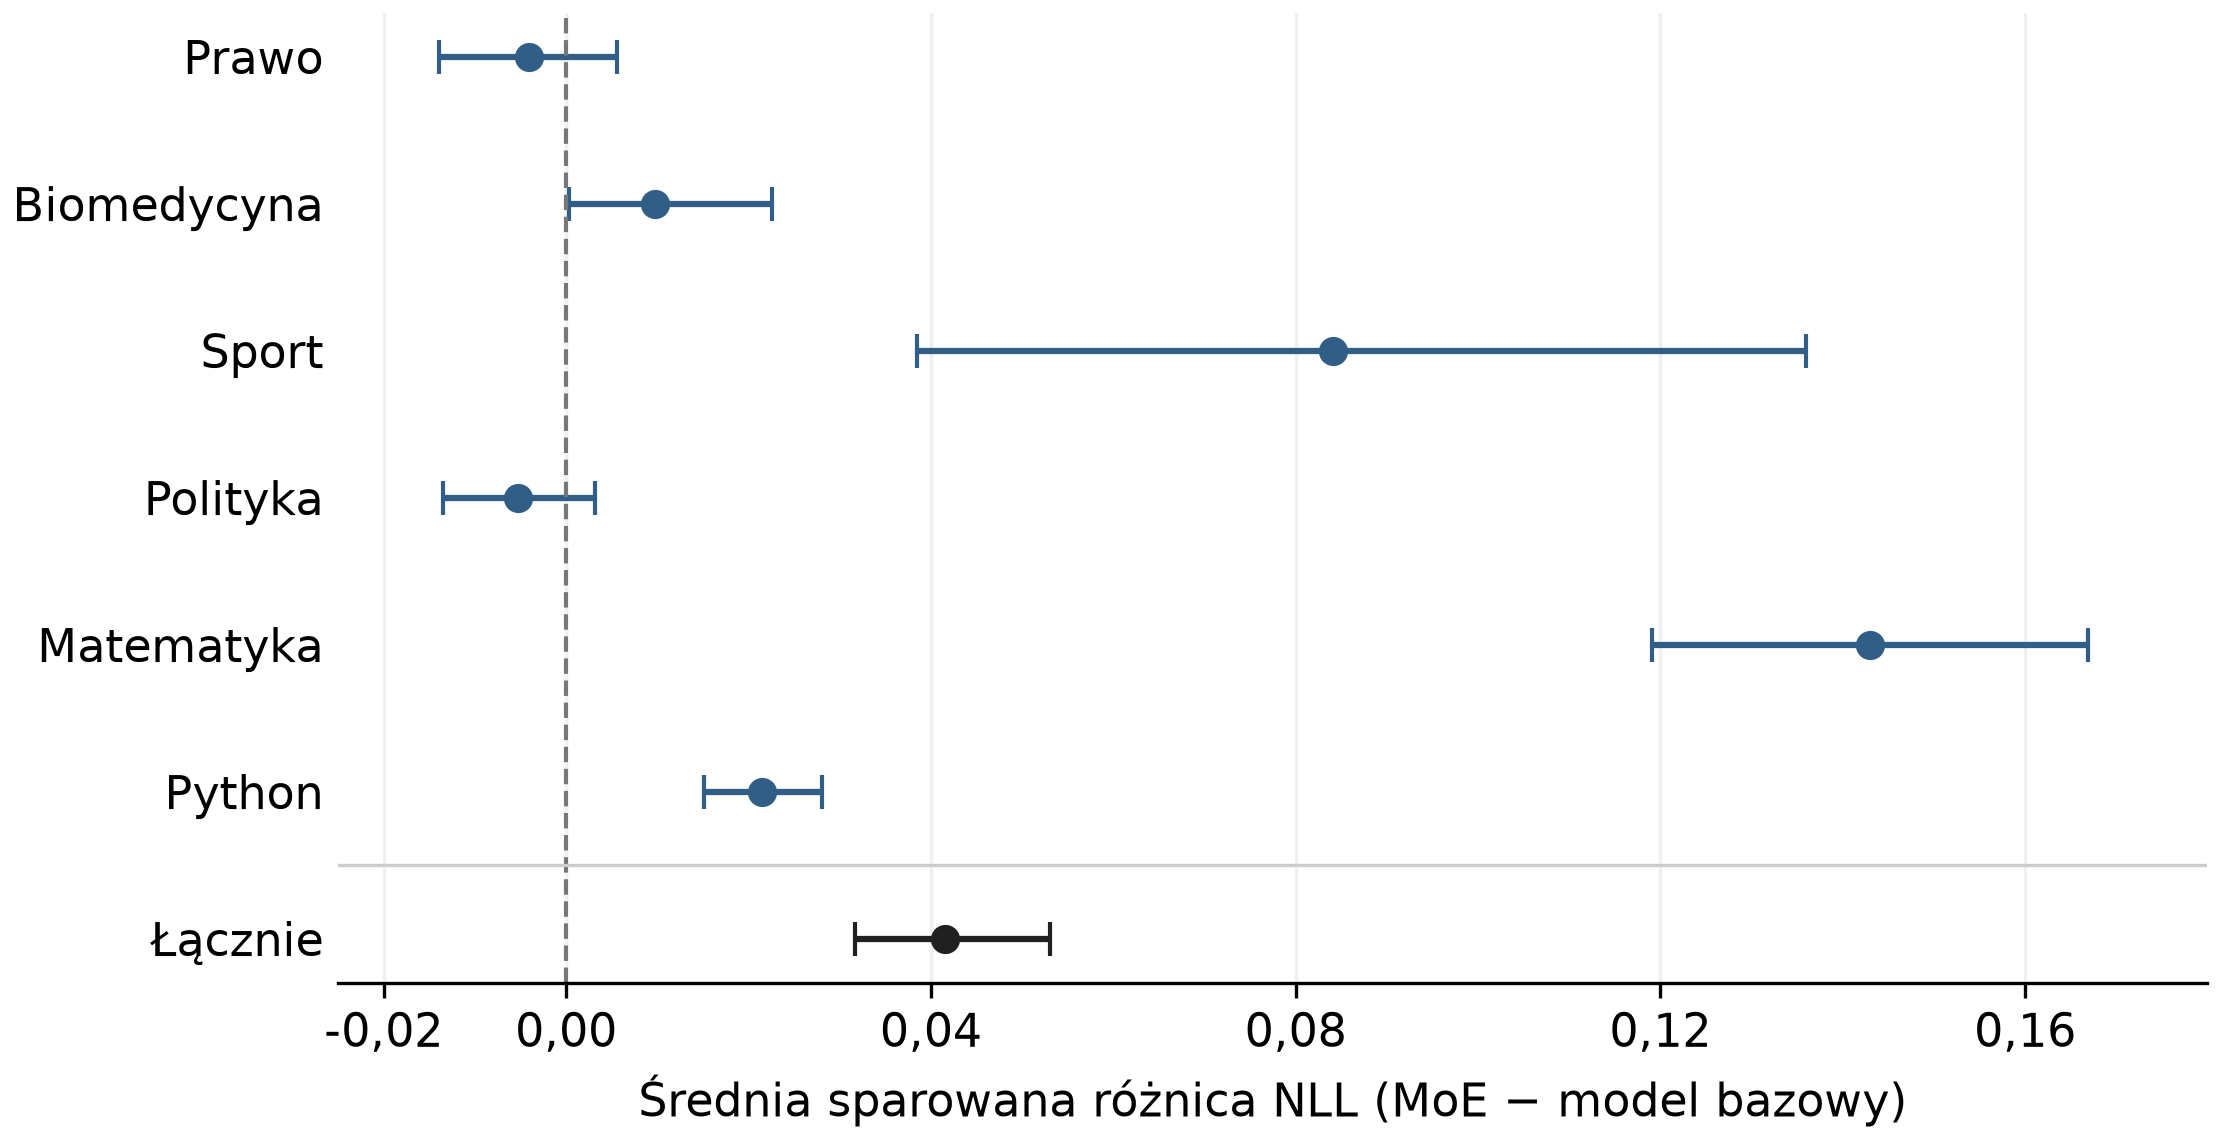
\includegraphics[width=\textwidth]{images/moe_validation_nll.png}
\caption{Średnie sparowane różnice NLL odpowiedzi referencyjnych wraz z przedziałami ufności $95\%$. Wartości dodatnie oznaczają pogorszenie MoE w benchmarku. Każda domena obejmuje $100$ przykładów, a wynik łączny -- $600$ przykładów o jednakowej wadze. Wykres opracowano na podstawie zapisanych wyników benchmarku.}
\label{fig:walidacja_nll}
\end{figure}

Przy nadaniu jednakowej wagi każdemu przykładowi wszystkie domeny mają taki sam udział w wyniku. Przy ważeniu liczbą tokenów odpowiedzi NLL wzrosło z $1{,}1818$ do $1{,}2277$, a PPL z $3{,}2603$ do $3{,}4135$, czyli o $4{,}70\%$. Tę agregację zdominował Python, obejmujący $6567$ spośród $7067$ tokenów odpowiedzi. Nie należy więc utożsamiać różnicy średnich ważonych tokenami ze średnią różnic dla przykładów przedstawioną na wykresie. \newline
Trafność odpowiedzi zmieniła się w znacznie mniejszym stopniu niż NLL (tabela~\ref{tab:walidacja_mc}). Łączna liczba trafień wzrosła ze $156$ do $158$ na $500$ pytań, czyli z $31{,}2\%$ do $31{,}6\%$. Przedział ufności dla zmiany wynosi $[-1{,}0;\,1{,}8]$ punktu procentowego. W polityce MoE poprawiło trzy odpowiedzi. Po uśrednieniu wyników dla różnych kolejności opcji trafność wzrosła z $30{,}67\%$ do $31{,}27\%$.

\begin{table}[htbp]
\centering
\begin{tabular}{lrrr}
\toprule
Domena & Model bazowy & MoE & Zmiana [p.p.] \\
\midrule
Prawo & $21\%$ & $20\%$ & $-1$ \\
Biomedycyna & $29\%$ & $29\%$ & $0$ \\
Sport & $50\%$ & $50\%$ & $0$ \\
Polityka & $35\%$ & $38\%$ & $+3$ \\
Matematyka & $21\%$ & $21\%$ & $0$ \\
\bottomrule
\end{tabular}
\caption{Trafność odpowiedzi modelu bazowego i MoE przy pierwotnej kolejności opcji, po $100$ pytań na domenę. Sport ma dwie opcje odpowiedzi, a pozostałe domeny po cztery.}
\label{tab:walidacja_mc}
\end{table}

Analiza kolejności odpowiedzi ujawniła to samo ograniczenie co w ocenie samodzielnych ekspertów. W sporcie baza i MoE wybierały A we wszystkich $200$ ocenach, a w matematyce we wszystkich $300$. Uzyskana trafność nie potwierdza zatem rozumienia zdań sportowych ani wykonywania działań arytmetycznych. Duży wzrost NLL oznacza mniejsze prawdopodobieństwo poprawnych etykiet, ale nie utratę wcześniej wykazanej umiejętności rozwiązywania tych zadań. W prawie, biomedycynie i polityce zgodność treści wybieranej odpowiedzi między kolejnościami opcji wynosiła jedynie około $55$--$57\%$, co również ogranicza interpretację trafności jako miary wiedzy. \newline
W generacji Pythona parsowalność kodu wyniosła $96\%$ dla bazy i $94\%$ dla MoE. W parach wystąpiły trzy poprawy i pięć pogorszeń, z $p\approx0{,}727$, więc wynik nie rozstrzyga o zmianie jakości składni. \newline
Na wspólnych zadaniach MoE uzyskało niższe średnie NLL niż właściwy samodzielny ekspert w pięciu domenach; wyjątkiem był sport. W Pythonie parsowalność wyniosła odpowiednio $94\%$ i $74\%$. Warunkowe użycie ekspertów ogranicza więc część pogorszeń obserwowanych przy stosowaniu przyciętego MLP do wszystkich tokenów. Nie dowodzi to przewagi samego routera: MoE korzysta również z nieprzyciętego MLP, a oba te elementy wpływają na wynik.


\section{Koszt obliczeń, generalizacja routera i ograniczenia wniosków}
\label{sec:generalizacja_routera}
\subsection{Koszt obliczeń modeli dziedzinowych}
\label{subsec:koszt_ekspertow}
Brak routera i fallbacku oznacza, że ekspert stale wykorzystuje $75\%$ szerokości badanego MLP. Redukuje to koszt projekcji tej warstwy o $25\%$, ale z racji na przeprowadzanie eksperymentu tylko na jednym bloku modelu, redukcja całkowita biorąc pod uwagę wszystkie warstwy MLP to jedynie około $1{,}389\%$. Liczba parametrów modelu z jednym ekspertem spada z $268\,098\,176$ do $267\,115\,136$, czyli o $0{,}367\%$. Zmierzona bazowa alokacja CUDA była niższa o $1{,}25$ MiB, natomiast zmiana szczytowej alokacji zależała od konfiguracji i nie zawsze była ujemna. 

\subsection{Koszt obliczeń i działanie routera w MoE}
\label{subsec:koszt_router_moe}
Telemetrię benchmarku MoE zbierano w osobnym przejściu przez same prompty, licząc każdy przykład jednokrotnie i pomijając padding. Nie obejmuje ona wielokrotnych ocen kandydatów w pytaniach wyboru ani kolejnych kroków generacji. Udziały routingu zestawiono w tabeli~\ref{tab:walidacja_routing}.

\begin{table}[htbp]
\centering
\small
\begin{tabular}{lrrr}
\toprule
Domena & Do ekspertów & Do zgodnego eksperta & Fallback \\
\midrule
Prawo & $22{,}10\%$ & $21{,}22\%$ & $77{,}90\%$ \\
Biomedycyna & $6{,}85\%$ & $4{,}76\%$ & $93{,}15\%$ \\
Sport & $24{,}53\%$ & $8{,}85\%$ & $75{,}47\%$ \\
Polityka & $3{,}65\%$ & $0{,}14\%$ & $96{,}35\%$ \\
Matematyka & $75{,}30\%$ & $75{,}30\%$ & $24{,}70\%$ \\
Python & $8{,}62\%$ & $0{,}11\%$ & $91{,}38\%$ \\
\bottomrule
\end{tabular}
\caption{Routing tokenów promptów w benchmarku MoE. Wszystkie odsetki są liczone względem ogółu tokenów danej domeny; kolumna zgodnego eksperta jest podzbiorem kolumny routingu do ekspertów.}
\label{tab:walidacja_routing}
\end{table}

Łącznie do ekspertów trafiło $19{,}64\%$ spośród $58\,246$ tokenów promptów, a pozostałe $80{,}36\%$ przetworzył bazowy MLP. Wśród skierowanych do ekspertów tokenów $84{,}79\%$ trafiło do eksperta zgodnego z domeną zadania, ale wynik ten jest zdominowany przez prawo i matematykę. W sporcie $616$ tokenów skierowano do matematyki, a tylko $348$ do sportu. W Pythonie były to odpowiednio $320$ tokenów skierowanych do matematyki i cztery do eksperta programistycznego. Do eksperta politycznego trafiło zaledwie $0{,}14\%$ tokenów zadań politycznych. Router może zatem częściowo rozpoznawać format tekstu zamiast jego dziedziny. Duży udział poprawnych skierowań w matematyce współistnieje z pogorszeniem NLL, więc sama zgodność eksperta z domeną nie gwarantuje jakości odpowiedzi. \newline
Duży udział sytuacji w której router nie wybierał eksperta tylko wracał do wariantu ogólnego ogranicza potencjalną oszczędność obliczeń. Korzystając z zależności wyprowadzonej w podrozdziale~\ref{sec:skladanie_moe}, otrzymano średnią efektywną szerokość zmodyfikowanego MLP równą $95{,}09\%$ szerokości bazowej. Dla trzech projekcji bramkowanego MLP koszt liniowy na token wynosi $C_{\mathrm{dense}}=3DH$, gdzie $D=640$ i $H=2048$. Po uwzględnieniu routera o sześciu wyjściach i udziału routingu $c$ przybliżony koszt ma postać:
\[
C_{\mathrm{MoE}}=(1-c)C_{\mathrm{dense}}+
0{,}75cC_{\mathrm{dense}}+6D.
\]
Przy zaobserwowanym routingu odpowiada to redukcji o około $4{,}81\%$ operacji mnożenia z akumulacją (ang. \textit{multiply--accumulate}, MAC) w MLP warstwy $9$. W odniesieniu do wszystkich $18$ modułów MLP jest to jedynie około $0{,}267\%$ ich łącznego kosztu liniowego. Udział w obliczeniach całego modelu jest jeszcze mniejszy, ponieważ pozostają mechanizmy uwagi i projekcja na słownik. \newline
Rachunek ten dotyczy rozkładu routingu zaobserwowanego na promptach, a nie zmierzonego kosztu pełnej generacji. Nie uwzględnia indeksowania tokenów, nieregularnych partii ekspertów ani transferów pamięci. Przechowywanie wag ekspertów obok bazowego MLP zwiększa zapotrzebowanie na pamięć; w badanej konfiguracji bazowa alokacja CUDA była większa o około $35{,}39$ MiB. Jest to konsekwencja zachowania pełnego MLP jako wariantu ogólnego, zgodnie z konstrukcją opisaną w rozdziale~\ref{chap:pruning_moe}. Architektura pozwala więc ograniczać liczbę operacji dla tokenów kierowanych do ekspertów, zachowując dostęp do nieprzyciętego modułu kosztem dodatkowej pamięci. \newline
Wyniki pokazują, że możliwe jest zbudowanie działającego MoE z ekspertów wyodrębnionych na podstawie domen semantycznych, przy zachowaniu trafności odpowiedzi i parsowalności kodu na poziomie zbliżonym do modelu bazowego. Ma to znaczenie w kontekście celu eksperymentu, ponieważ każdy wybrany ekspert wykorzystuje MLP o szerokości zmniejszonej o $25\%$. Usunięcie części neuronów może pogarszać jakość przewidywania, dlatego ograniczenie skali tego pogorszenia przy mniejszej liczbie operacji stanowi korzystny rezultat. \newline
W benchmarku zadań domenowych PPL MoE ważone liczbą tokenów wzrosło o $4{,}70\%$, a zmiany trafności odpowiedzi i parsowalności kodu były niewielkie i statystycznie nierozstrzygające. Wyniki wskazują zatem na zachowanie znacznej części jakości mierzonej tymi wskaźnikami. Nie oznacza to jednak jednakowo małego pogorszenia w każdej domenie: wzrost NLL był większy w sporcie i matematyce, a zależność wyboru odpowiedzi od jej pozycji ogranicza ocenę rzeczywistych umiejętności modelu. MoE uzyskało niższe średnie NLL niż samodzielni eksperci w pięciu z sześciu domen, co wskazuje na korzyść z warunkowego stosowania przyciętych modułów wraz z zachowaniem bazowego MLP. \newline
Mniejsza liczba mnożeń daje możliwość przyspieszenia obliczeń, ale jej wykorzystanie zależy od organizacji danych, rozdzielania tokenów między ekspertów i efektywności mnożenia macierzy na GPU. Optymalizacja tych elementów wykracza poza zakres pracy. Przedstawiona analiza określa zatem teoretyczną redukcję liczby operacji, bez utożsamiania jej z przyspieszeniem całego modelu.


\chapter{Podsumowanie i~wnioski}

\section{Weryfikacja możliwości wydzielenia wiedzy bez znacznej utraty jakości w danej dziedzinie}

\section{Perspektywy inżynieryjne: minimalizacja narzutu obliczeniowego przy bramkowaniu rzadkich podsieci}

\addcontentsline{toc}{chapter}{Bibliografia}
\bibliographystyle{unsrt}
\bibliography{bibliografia}

% Aneksy z interpretacją cech:
\appendix
\chapter{Katalog wybranych cech modelu \textit{Pythia}}
\label{appendix:katalog_cech_pythia}
Niniejszy aneks zawiera opisy i interpretacje wybranych cech wyekstrahowanych przez autoenkoder dla modelu \textit{Pythia} z warstwy $6$ modelu \textit{Pythia~160M}. Opis każdej z cech obejmuje: identyfikator cechy w słowniku autoenkodera, proponowaną interpretację semantyczną, zbiór tokenów aktywujących cechę, wraz z liczbą wystąpień w zbiorze użytym do analizy, tokeny które dana cecha promuje (te które mają największą szansę zostać przez nią wygenerowane), wraz z wartością \textit{logit lens} wspierania danego tokenu oraz przykłady fragmentów tekstu z wysoką wartością aktywacji. \newline
Zbiór \textit{The Pile} na którym prowadzona była analiza jest zbiorem w całości w języku angielskim. Z tego też powodu wszystkie przykłady, zarówno tokenów aktywizujących i generowanych oraz przykłady w tekście przedstawione są również w języku angielskim. \newline
Cechy dobrano tak, aby reprezentować różnorodne kategorie semantyczne -- od koncepcji wąskich i wysoce wyspecjalizowanych po wzorce o szerokim zasięgu -- co ilustruje przekrój reprezentacji kodowanych przez model.
%TODO: dodać aneksy także dla Gemma i Tinystories

% definicja środowiska karty cechy
\tcbset{
  featurestyle/.style={
    enhanced,
    colback=gray!4,
    colframe=gray!50!black,
    coltitle=white,
    fonttitle=\sffamily\bfseries\small,
    left=4pt, right=4pt, top=3pt, bottom=3pt,
    toptitle=3pt, bottomtitle=2pt,
    boxrule=0.6pt,
    arc=2pt,
    breakable=false,
    before upper={\setstretch{1.0}\fontsize{10}{12}\selectfont},
  }
}
% makro pomocnicze: linia sekcji wewnątrz karty
\newcommand{\featurefield}[1]{%
  \par\vspace{3pt}%
  {\sffamily\bfseries\small\color{gray!70!black}#1}\par\vspace{1pt}%
}
\newcommand{\tok}[1]{\texttt{\textquotesingle#1\textquotesingle}}
\newcommand{\hltoken}[1]{\colorbox{yellow!30}{\textbf{#1}}}

% ============================================================
%  CECHA #5907
% ============================================================
\begin{tcolorbox}[featurestyle,
  title={Cecha \texttt{\#5907} \hfill Terminy z dziedziny fotoniki}]
\featurefield{Interpretacja}
Cecha silnie promuje tokeny związane z dziedziną fotoniki oraz właściwościami i terminami opisującymi promieniowanie elektromagnetyczne.
\featurefield{Tokeny aktywujące \normalfont (token $\to$ liczba wystąpień)}
\begin{tabular}{@{}l r@{\qquad}l r@{\qquad}l r@{\qquad}l r@{}}
\tok{ the}   & 48\,925 & \tok{ of}  & 27\,250 & \tok{ a}    & 17\,680 & \tok{ (}  & 16\,178 \\
\tok{ ,}     & 14\,558 & \tok{ to}  & 12\,588 & \tok{ at}   & 12\,143 & \tok{ in} & 11\,309 \\
\end{tabular}
\featurefield{Tokeny generowane \normalfont (token $\to$ wsparcie)}
\begin{tabular}{@{}l r@{\qquad}l r@{}}
\tok{ wavelengths}  & $+$0,247 & \tok{ photons}    & $+$0,225 \\
\tok{ photon}       & $+$0,214 & \tok{ brightest}  & $+$0,211 \\
\tok{ wavelength}   & $+$0,211 & \tok{ beam}       & $+$0,210 \\
\tok{ spectra}      & $+$0,209 & \tok{ radiation}  & $+$0,206 \\
\end{tabular}
\featurefield{Przykłady aktywacji}
\begin{tabular}{@{}p{0.18\linewidth} p{0.75\linewidth}@{}}
\tok{ emission}  & \texttt{...confocal imaging suite with lasers tuned to the\hltoken{ emission} spectra of the secondary fluorescent antibodies...} \\[3pt]
\tok{ laser}     & \texttt{...Red fluorophore (A546) was excited with a diode\hltoken{ laser} (561\,nm) and DAPI was excited with a 405...} \\[3pt]
\tok{ radiation} & \texttt{...monochromatic X ray (1486.7\,eV, Al K$\alpha$)\hltoken{ radiation} was used to generate photoelectron spectra...} \\
\end{tabular}
\end{tcolorbox}

% ============================================================
%  CECHA #7135
% ============================================================
\begin{tcolorbox}[featurestyle,
  title={Cecha \texttt{\#7135} \hfill Rozszerzenia plików}]
\featurefield{Interpretacja}
Cecha aktywuje się przede wszystkim w miejscach występowania końca zdania, a jednocześnie promuje tokeny będące rozszerzeniami plików oraz nazwami metod i elementów stosowanych w programowaniu.
\featurefield{Tokeny aktywujące \normalfont (token $\to$ liczba wystąpień)}
\begin{tabular}{@{}l r@{\qquad}l r@{\qquad}l r@{\qquad}l r@{}}
\tok{ .} & 929\,620 & \tok{ ,} & 23\,635 & \tok{.} & 21\,092 & \tok{ ...} & 6\,752 \\
\tok{ !} & 4\,388 & \tok{ )} & 3\,088 & \tok{ ?} & 3\,034 & \tok{ ’} & 1\,651 \\
\end{tabular}
\featurefield{Tokeny generowane \normalfont (token $\to$ wsparcie)}
\begin{tabular}{@{}l r@{\qquad}l r@{}}
\tok{unnumbered} & $+$0,446 & \tok{NET} & $+$0,295 \\
\tok{innerHTML} & $+$0,229 & \tok{tgz} & $+$0,221 \\
\tok{csv} & $+$0,220 & \tok{exe} & $+$0,218 \\
\tok{toString} & $+$0,210 & \tok{gif} & $+$0,208 \\
\end{tabular}
\featurefield{Przykłady aktywacji}
\begin{tabular}{@{}p{0.18\linewidth} p{0.75\linewidth}@{}}
\tok{ .} & \texttt{...Without restraints or controls ; uninhibited\hltoken{ .}\# * * unrestricted...} \\[3pt]
\tok{ .} & \texttt{...the actual binary\hltoken{ .}You should change the target to refer to the main binary...} \\[3pt]
\tok{ .} & \texttt{...Download a\hltoken{ .} osm file of the area you want...} \\
\end{tabular}
\end{tcolorbox}

% ============================================================
%  CECHA #1047
% ============================================================
\begin{tcolorbox}[featurestyle,
  title={Cecha \texttt{\#1047} \hfill Przeciwności i przeciwnicy}]
\featurefield{Interpretacja}
Cecha aktywuje się w kontekstach konfliktu, walki i przeciwstawiania się komuś lub czemuś, obejmując zarówno bezpośrednich przeciwników, jak i abstrakcyjne przeciwności.
\featurefield{Tokeny aktywujące \normalfont (token $\to$ liczba wystąpień)}
\begin{tabular}{@{}l r@{\qquad}l r@{\qquad}l r@{\qquad}l r@{}}
\tok{ of} & 24\,441 & \tok{ the} & 16\,956 & \tok{ to} & 16\,715 & \tok{ with} & 7\,528 \\
\tok{ for} & 7\,219 & \tok{ in} & 6\,949 & \tok{ against} & 6\,783 & \tok{ on} & 6\,613 \\
\end{tabular}
\featurefield{Tokeny generowane \normalfont (token $\to$ wsparcie)}
\begin{tabular}{@{}l r@{\qquad}l r@{}}
\tok{ against} & $+$0,154 & \tok{ Against} & $+$0,100 \\
% W analizie występuje tu znak zastępczy Unicode U+FFFD; zapis tekstowy
% pozwala zachować informację o tokenie bez błędu kompilacji pdfLaTeX.
\tok{ contre} & $+$0,082 & \tok{U+FFFD} & $+$0,072 \\
\tok{against} & $+$0,065 & \tok{ backdrop} & $+$0,039 \\
\tok{ opponents} & $+$0,036 & \tok{ opponent} & $+$0,033 \\
\end{tabular}
\featurefield{Przykłady aktywacji}
\begin{tabular}{@{}p{0.18\linewidth} p{0.75\linewidth}@{}}
\tok{ battle} & \texttt{...a face of a titanic\hltoken{ battle} in Florida over a racist bill...} \\[3pt]
\tok{ fight} & \texttt{...the continuing\hltoken{ fight} for freedom and equality...} \\[3pt]
\tok{ fought} & \texttt{...So I was thrown into teaching and I\hltoken{ fought} it for years...} \\
\end{tabular}
\end{tcolorbox}

% ============================================================
%  CECHA #4716
% ============================================================
\begin{tcolorbox}[featurestyle,
  title={Cecha \texttt{\#4716} \hfill Regulacje i ograniczenia}]
\featurefield{Interpretacja}
Cecha reprezentuje pojęcia regulacji, nadzoru i nakładania ograniczeń, w szczególności w kontekstach prawnych, administracyjnych i technicznych.
\featurefield{Tokeny aktywujące \normalfont (token $\to$ liczba wystąpień)}
\begin{tabular}{@{}l r@{\qquad}l r@{\qquad}l r@{\qquad}l r@{}}
\tok{ to} & 17\,328 & \tok{ of} & 16\,920 & \tok{ the} & 15\,973 & \tok{ for} & 8\,208 \\
\tok{ a} & 6\,749 & \tok{ must} & 5\,955 & \tok{ set} & 5\,553 & \tok{ control} & 5\,524 \\
\end{tabular}
\featurefield{Tokeny generowane \normalfont (token $\to$ wsparcie)}
\begin{tabular}{@{}l r@{\qquad}l r@{}}
\tok{ imposed} & $+$0,456 & \tok{ governing} & $+$0,392 \\
\tok{ enforced} & $+$0,389 & \tok{ violations} & $+$0,361 \\
\tok{ set} & $+$0,359 & \tok{ conditions} & $+$0,357 \\
\tok{ promul} & $+$0,345 & \tok{ compliance} & $+$0,341 \\
\end{tabular}
\featurefield{Przykłady aktywacji}
\begin{tabular}{@{}p{0.18\linewidth} p{0.75\linewidth}@{}}
\tok{ restriction} & \texttt{...there was not and had never been any\hltoken{ restriction} at all on cross examining...} \\[3pt]
\tok{ limits} & \texttt{...public health experts who say that stringent\hltoken{ limits} must be established by government regulators...} \\[3pt]
\tok{ prohibition} & \texttt{...acknowledged , despite a religious\hltoken{ prohibition} against the use of electronics...} \\
\end{tabular}
\end{tcolorbox}

% ============================================================
%  CECHA #9003
% ============================================================
\begin{tcolorbox}[featurestyle,
  title={Cecha \texttt{\#9003} \hfill Nawiasowanie i zagnieżdżanie wyrażeń}]
\featurefield{Interpretacja}
Cecha aktywuje się w wyrażeniach o silnie zagnieżdżonej strukturze, zwłaszcza w rachunkach i kodzie zawierających nawiasy, nawiasy kwadratowe oraz klamrowe.
\featurefield{Tokeny aktywujące \normalfont (token $\to$ liczba wystąpień)}
\begin{tabular}{@{}l r@{\qquad}l r@{\qquad}l r@{\qquad}l r@{}}
\tok{ \}} & 70\,549 & \tok{ )} & 41\,197 & \tok{ (} & 36\,081 & \tok{ \textbackslash} & 33\,306 \\
\tok{ \{} & 30\,271 & \tok{ "} & 27\,835 & \tok{ ,} & 23\,035 & \tok{ 1} & 21\,077 \\
\end{tabular}
\featurefield{Tokeny generowane \normalfont (token $\to$ wsparcie)}
\begin{tabular}{@{}l r@{\qquad}l r@{}}
\tok{]],} & $+$0,227 & \tok{'])} & $+$0,205 \\
\tok{]]} & $+$0,205 & \tok{)),} & $+$0,199 \\
\tok{)):} & $+$0,190 & \tok{)))} & $+$0,182 \\
\tok{]\{\}]\{\}} & $+$0,179 & \tok{]))} & $+$0,168 \\
\end{tabular}
\featurefield{Przykłady aktywacji}
\begin{tabular}{@{}p{0.18\linewidth} p{0.75\linewidth}@{}}
\tok{ 99} & \texttt{...sqrt ( 11 ) - ( sqrt (\hltoken{ 99} ) - ( 1 + ( sqrt ( 99 )...} \\[3pt]
\tok{ 72} & \texttt{...sqrt ( 8 ) - ( 2*sqrt (\hltoken{ 72} ) + sqrt ( 8 )...} \\[3pt]
\tok{125} & \texttt{...sqrt ( 1125 ) - ( sqrt ( 1\hltoken{125} ) )...} \\
\end{tabular}
\end{tcolorbox}

% ============================================================
%  CECHA #4308
% ============================================================
\begin{tcolorbox}[featurestyle,
  title={Cecha \texttt{\#4308} \hfill Więzienie i sytuacje osadzenia}]
\featurefield{Interpretacja}
Cecha jest związana z więzieniem, osadzonymi i pozbawieniem wolności, a także z sytuacjami kryzysowymi często występującymi w opisach przemocy, śmierci i interwencji ratunkowej.
\featurefield{Tokeny aktywujące \normalfont (token $\to$ liczba wystąpień)}
\begin{tabular}{@{}l r@{\qquad}l r@{\qquad}l r@{\qquad}l r@{}}
\tok{ the} & 34\,335 & \tok{ of} & 25\,417 & \tok{ to} & 20\,194 & \tok{ a} & 17\,851 \\
\tok{ in} & 16\,581 & \tok{ was} & 15\,223 & \tok{ and} & 13\,009 & \tok{ ,} & 10\,885 \\
\end{tabular}
\featurefield{Tokeny generowane \normalfont (token $\to$ wsparcie)}
\begin{tabular}{@{}l r@{\qquad}l r@{}}
\tok{ awaiting} & $+$0,213 & \tok{ prisoners} & $+$0,184 \\
\tok{ prisoner} & $+$0,179 & \tok{ waiting} & $+$0,176 \\
\tok{ ambulance} & $+$0,175 & \tok{ rescue} & $+$0,175 \\
\tok{ wounds} & $+$0,165 & \tok{ inmate} & $+$0,162 \\
\end{tabular}
\featurefield{Przykłady aktywacji}
\begin{tabular}{@{}p{0.18\linewidth} p{0.75\linewidth}@{}}
\tok{ death} & \texttt{...some ten million of whom starved to\hltoken{ death} in five years...} \\[3pt]
\tok{ care} & \texttt{...His sister is in intensive\hltoken{ care} , struggling for her sight...} \\[3pt]
\tok{ hospital} & \texttt{...another victim of weekend shootings died in\hltoken{ hospital}...} \\
\end{tabular}
\end{tcolorbox}

% ============================================================
%  CECHA #6899
% ============================================================
\begin{tcolorbox}[featurestyle,
  title={Cecha \texttt{\#6899} \hfill Dawki leków}]
\featurefield{Interpretacja}
Cecha promuje pojęcia związane z dawkowaniem i podawaniem leków, obejmując dawki, schematy leczenia, terapię oraz substancje farmakologiczne.
\featurefield{Tokeny aktywujące \normalfont (token $\to$ liczba wystąpień)}
\begin{tabular}{@{}l r@{\qquad}l r@{\qquad}l r@{\qquad}l r@{}}
\tok{ ,} & 36\,462 & \tok{ .} & 25\,311 & \tok{ of} & 24\,685 & \tok{ )} & 20\,702 \\
\tok{ in} & 20\,361 & \tok{ (} & 19\,634 & \tok{ and} & 18\,408 & \tok{ the} & 17\,211 \\
\end{tabular}
\featurefield{Tokeny generowane \normalfont (token $\to$ wsparcie)}
\begin{tabular}{@{}l r@{\qquad}l r@{}}
\tok{ doses} & $+$0,317 & \tok{ dose} & $+$0,289 \\
\tok{ dosage} & $+$0,289 & \tok{ administered} & $+$0,267 \\
\tok{ dosing} & $+$0,257 & \tok{ analgesic} & $+$0,254 \\
\tok{ regimens} & $+$0,250 & \tok{ therapy} & $+$0,242 \\
\end{tabular}
\featurefield{Przykłady aktywacji}
\begin{tabular}{@{}p{0.18\linewidth} p{0.75\linewidth}@{}}
\tok{ drug} & \texttt{...information about gene systems important for modulating\hltoken{ drug} responses...} \\[3pt]
\tok{ administered} & \texttt{...restores beta cell function and reverts oxidative stress .When\hltoken{ administered} , in a period...} \\[3pt]
\tok{ antagonists} & \texttt{...the pathophysiology of heart failure .Mineralocorticoid receptor\hltoken{ antagonists} have thus emerged...} \\
\end{tabular}
\end{tcolorbox}

% ============================================================
%  CECHA #347
% ============================================================
\begin{tcolorbox}[featurestyle,
  title={Cecha \texttt{\#347} \hfill Partie polityczne i ruchy polityczne}]
\featurefield{Interpretacja}
Cecha reprezentuje partie polityczne, ruchy polityczne i ich uczestników, ze szczególnym uwzględnieniem określeń opisujących radykalizm, orientację polityczną i aktywizm.
\featurefield{Tokeny aktywujące \normalfont (token $\to$ liczba wystąpień)}
\begin{tabular}{@{}l r@{\qquad}l r@{\qquad}l r@{\qquad}l r@{}}
\tok{ the} & 38\,260 & \tok{ ,} & 30\,855 & \tok{ of} & 25\,684 & \tok{ to} & 18\,666 \\
\tok{ and} & 14\,420 & \tok{ .} & 14\,312 & \tok{ a} & 13\,122 & \tok{ in} & 11\,452 \\
\end{tabular}
\featurefield{Tokeny generowane \normalfont (token $\to$ wsparcie)}
\begin{tabular}{@{}l r@{\qquad}l r@{}}
\tok{ party} & $+$0,267 & \tok{ Party} & $+$0,264 \\
\tok{party} & $+$0,229 & \tok{ leader} & $+$0,229 \\
\tok{ militant} & $+$0,220 & \tok{ activists} & $+$0,218 \\
\tok{atism} & $+$0,215 & \tok{ movement} & $+$0,213 \\
\end{tabular}
\featurefield{Przykłady aktywacji}
\begin{tabular}{@{}p{0.18\linewidth} p{0.75\linewidth}@{}}
\tok{ radical} & \texttt{...the statement reiterated his\hltoken{ radical} views .“ We , the mujahedeen...} \\[3pt]
\tok{ right} & \texttt{...Europe ’s “ poster child for the far\hltoken{ right} ”...} \\[3pt]
\tok{ nationalist} & \texttt{...The Namibia National Front was an alliance of\hltoken{ nationalist} but moderate parties...} \\
\end{tabular}
\end{tcolorbox}

% ============================================================
%  CECHA #256
% ============================================================
\begin{tcolorbox}[featurestyle,
  title={Cecha \texttt{\#256} \hfill Rynek finansowy}]
\featurefield{Interpretacja}
Cecha jest związana z rynkiem finansowym i działalnością inwestycyjną, obejmując ceny, inwestorów, spółki, sprzedaż oraz portfele aktywów.
\featurefield{Tokeny aktywujące \normalfont (token $\to$ liczba wystąpień)}
\begin{tabular}{@{}l r@{\qquad}l r@{\qquad}l r@{\qquad}l r@{}}
\tok{ of} & 20\,085 & \tok{ the} & 19\,306 & \tok{ in} & 13\,893 & \tok{ a} & 10\,213 \\
\tok{ for} & 8\,126 & \tok{s} & 7\,508 & \tok{ ,} & 6\,947 & \tok{ and} & 5\,596 \\
\end{tabular}
\featurefield{Tokeny generowane \normalfont (token $\to$ wsparcie)}
\begin{tabular}{@{}l r@{\qquad}l r@{}}
\tok{ prices} & $+$0,094 & \tok{ investors} & $+$0,093 \\
\tok{owner} & $+$0,092 & \tok{ markets} & $+$0,090 \\
\tok{ selling} & $+$0,089 & \tok{ companies} & $+$0,087 \\
\tok{ investor} & $+$0,087 & \tok{ portfolio} & $+$0,086 \\
\end{tabular}
\featurefield{Przykłady aktywacji}
\begin{tabular}{@{}p{0.18\linewidth} p{0.75\linewidth}@{}}
\tok{ market} & \texttt{...The\hltoken{ market} for electronic devices continually demands higher performance...} \\[3pt]
\tok{ business} & \texttt{...Flora Mac Rinnalch , who ran a\hltoken{ business} selling timber...} \\[3pt]
\tok{ sell} & \texttt{...one of just two analysts with a\hltoken{ sell} rating on the stock...} \\
\end{tabular}
\end{tcolorbox}

% ============================================================
%  CECHA #2308
% ============================================================
\begin{tcolorbox}[featurestyle,
  title={Cecha \texttt{\#2308} \hfill Publikacje naukowe}]
\featurefield{Interpretacja}
Cecha aktywuje się w opisach publikacji naukowych, ich celów i zakresu, a także w sformułowaniach typowych dla abstraktów i prezentacji wyników badań.
\featurefield{Tokeny aktywujące \normalfont (token $\to$ liczba wystąpień)}
\begin{tabular}{@{}l r@{\qquad}l r@{\qquad}l r@{\qquad}l r@{}}
\tok{ the} & 61\,911 & \tok{ ,} & 49\,346 & \tok{ .} & 38\,923 & \tok{ of} & 34\,125 \\
\tok{ to} & 28\,983 & \tok{ is} & 24\,969 & \tok{ a} & 24\,850 & \tok{ and} & 21\,947 \\
\end{tabular}
\featurefield{Tokeny generowane \normalfont (token $\to$ wsparcie)}
\begin{tabular}{@{}l r@{\qquad}l r@{}}
\tok{abstract} & $+$0,147 & \tok{ aims} & $+$0,112 \\
\tok{ focus} & $+$0,109 & \tok{ foc} & $+$0,106 \\
\tok{ focused} & $+$0,100 & \tok{ focuses} & $+$0,096 \\
\tok{Abstract} & $+$0,096 & \tok{ abstract} & $+$0,093 \\
\end{tabular}
\featurefield{Przykłady aktywacji}
\begin{tabular}{@{}p{0.18\linewidth} p{0.75\linewidth}@{}}
\tok{ paper} & \texttt{...The present\hltoken{ paper} focuses on RWRE on a regular rooted tree...} \\[3pt]
\tok{ study} & \texttt{...In this context , the present\hltoken{ study} aims at characterizing IVD aging...} \\[3pt]
\tok{ study} & \texttt{...the present\hltoken{ study} was undertaken to determine their prevalence...} \\
\end{tabular}
\end{tcolorbox}
\input{appendices/B_katalog_cech_gemma}

\end{document}
